\begin{abstract}

Cytolytic T cell responses are predicted to be biased towards membrane proteins. 
The peptide-binding grooves of the alleles of most haplotypes
of histocompatibility complex class I (MHC-I) are relatively hydrophobic, 
therefore peptide fragments derived from human transmembrane helices (TMHs) are predicted to be presented more often as would be expected 
based on their abundance in the proteome. However, the physiological reason of why membrane proteins might be over-presented is unclear. 
In this study, we show that the predicted over-presentation of TMH-derived peptides is general, as it is predicted for bacteria and viruses 
and for both MHC-I and MHC-II, and confirmed from re-analysis of epitope databases. Moreover, we show that TMHs are evolutionarily more conserved, 
because single nucleotide polymorphisms (SNPs) are present 
relatively less frequently in TMH-coding chromosomal regions 
compared to regions coding for extracellular and cytoplasmic protein regions. 
Thus, our findings suggest that 
both cytolytic and helper T cells respond more to membrane proteins, 
because these are evolutionary more conserved. 
We speculate that TMHs therefore are less prone to escape mutations 
that enable pathogens to evade T cell responses.

\end{abstract}

{\bf Keywords:} antigen presentation, membrane proteins, bioinformatics, 
adaptive immunity, transmembrane domain, transmembrane helix, 
epitopes, T lymphocyte, MHC-I, MHC-II, evolutionary conservation

%%%%%%%%%%%%%%%%%%%%%%%%%%%%%%%%%%%%%%%%%%%%%%%%%%%%%%%%%%%%%%%%%%%%%%%%%%%%%%%%
\section*{Abbreviations}
%%%%%%%%%%%%%%%%%%%%%%%%%%%%%%%%%%%%%%%%%%%%%%%%%%%%%%%%%%%%%%%%%%%%%%%%%%%%%%%%

\begin{table}[h]
  \begin{tabular}{ll}
    Abbreviation & Full               \\ 
    \hline
ER & Endoplasmatic reticulum \\
ERAD & ER-associated degradation \\
HLA & Human leukocyte antigen \\
IEDB & Immune Epitope Database  \\
LB & lipid body \\
MAP & Membrane-associated protein \\
MHC & Major histocompatibility complex \\
MVB & Multivesicular body \\
PLC & Peptide-loading complex \\
SNP & Single nucleotide polymorphism \\
TMH & Transmembrane helix         \\
    TMP & Transmembrane protein
  \end{tabular}
\end{table}

%%%%%%%%%%%%%%%%%%%%%%%%%%%%%%%%%%%%%%%%%%%%%%%%%%%%%%%%%%%%%%%%%%%%%%%%%%%%%%%%
\section{Introduction}
%%%%%%%%%%%%%%%%%%%%%%%%%%%%%%%%%%%%%%%%%%%%%%%%%%%%%%%%%%%%%%%%%%%%%%%%%%%%%%%%

% \paragraph{Immune response}

Our immune system fights diseases and infections from pathogens, 
such as fungi, bacteria or viruses. 
An important part of the acquired immune response, 
that develops specialized and more specific recognition of pathogens 
than the innate immune response, 
is T cells which recognize peptides, called epitopes, derived from antigenic proteins presented on Major Histocompatibility Complexes (MHC) class I and II on the cell surface. 

% \paragraph{Classification of HLA}

The MHC proteins are heterodimeric complexes encoded by the
HLA (Human Leukocyte Antigens) genes.
In humans, the peptide binding groove of MHC-I is made by only the alpha subunit. There are three classical haplotypes of MHC-I, hallmarked by a highly polymorphic alpha chain called HLA-A, HLA-B and HLA-C, that all present epitopes to cytolytic T cells. 
For MHC-II, both the alpha and the beta chains contribute to the peptide binding groove. There are three classical haplotypes of MHC-II as well, called HLA-DR, HLA-DQ and HLA-DP, that all present epitopes to helper T cells.
Each MHC complex can present a subset of all possible peptides.
For example, HLA-A and HLA-B have no overlap in which
epitopes they bind \cite{lund2004definition}.
Moreover, the HLA genes of humans are highly polymorphic, with hundreds 
to thousands of different alleles, 
and each different allele presents a different subset of peptides \cite{marsh2010nomenclature}.

% \paragraph{HLAs increase detection range}

Humans mostly express two alleles per MHC haplotype, one from the parental and one from the maternal chromosome, 
and therefore an individual's immune system detects 
only a fraction of all possible peptide fragments. 
However, at the population level, the coverage of pathogenic peptides that are detected 
is very high, because of the highly polymorphic MHC genes.
It is therefore believed that MHC polymorphism improves immunity at the population level, 
as mutations in a protein that disrupt a particular MHC presentation at the individual level, 
so-called escape mutations, 
will not affect MHC presentation for all alleles present in the population \cite{sommer2005importance}.

% \paragraph{Epitope prediction}

Many studies are aimed at identifying the repertoire of epitopes that are presented 
in any of the different alleles to determine which epitopes will result in an immune response, 
as this will for instance aid the design of vaccines. 
These studies have led to the development of prediction algorithms 
that allow for very reliable \emph{in silico} predictions 
of the binding affinities of peptides
\cite{larsen2010identification,schellens2008unanticipated,tang2011genome}.
For example, S. Tang et al. \cite{tang2011genome} found that, 
of the 432 peptides that were predicted to bind to an MHC allele,
86\% were experimentally confirmed to do so. 

% \paragraph{TMHs}

Using these prediction algorithms, 
we recently predicted that peptides derived 
from transmembrane helices (TMHs) 
are likely to be more frequently presented by MHC-I 
than expected based on their abundance \cite{bianchi2017},
which is in line with a previous study 
by Istrail et al \cite{istrail2004comparative},
demonstrating that N-terminal signal sequences 
are likely to be presented within major histocompatibility complexes, 
due their hydrophobic nature. 
Moreover, we showed that some well-known immunodominant peptides stem from TMHs. 
This over-presentation is attributed to the fact 
that the peptide-binding groove of most MHC-I alleles
is relatively hydrophobic, 
and therefore hydrophobic TMH-derived peptides have a higher affinity 
to bind than their soluble hydrophilic counterparts. 

TMHs are hydrophobic 
as they need to span the hydrophobic lipid bilayer of cellular membranes.
They consist of an alpha helix of, on average, 23 amino acids in length. 
TMHs can also be predicted with high accuracy from a protein sequence 
by bioinformatics approaches \cite{krogh2001predicting,kall2004combined,arai2004conpred,jones2007improving,klammer2009metatm,wang2019efficient}. For example, a study by Jones \cite{jones2007improving} found that,
from 184 transmembrane proteins (TMPs) with known topology, 
80\% of the TMH predictions replicated this finding.
 
TMHs are common structures in the proteins of humans and microbes. 
Different TMH prediction tools estimate that 15-39\% of all proteins 
in the human proteome contain at least one TMH \cite{ahram2006estimation}.
However, the physiological reason why peptides derived from TMHs 
would be presented more often than peptides 
stemming from soluble (i.e., extracellular or cytoplasmic) protein regions is unknown. 
In this study, we hypothesized that the presentation of 
TMH residues is evolutionary selected for, 
because TMHs are less prone to undergo escape mutations. 
One reason to expect such a reduced 
variability (and hence evolutionary conservation) in TMHs, 
is that these are restricted in their evolution 
by the functional requirement to span a lipid bilayer. 
Due to this requirement, 
many of the amino acids genuinely present in TMHs 
are limited to the ones with hydrophobic side chains 
\cite{hessa2007molecular,jones1994model}.
Therefore, we speculated that the TMHs of pathogens 
might have a lower chance to develop escape mutations, 
as many mutations will result in a dysfunctional TMH 
and render the protein inactive.

This study had two objectives. 
First, we aimed to generalize our findings by predicting the presentation of peptides 
from different kingdoms of life and for both MHC-I and -II. 
From these \emph{in silico} predictions, we conclude that TMH-derived
epitopes are likely to be presented more often than expected by chance,
in a human, viral and bacterial proteome, 
and for most alleles of both MHC-I and II. 
We confirmed the presentation of TMH-derived peptides 
by re-analysis of peptide elution studies. 
Second, we tested our hypothesis that TMHs 
are more evolutionary conserved than soluble protein regions. 
Our analysis of human single nucleotide polymorphisms (SNPs) showed 
that random point mutations are indeed less likely
to occur within TMHs. 
These findings strengthen the emerging notion 
that TMHs are important for the T cell branch of the adaptive immune system, 
and hence are of  
overlooked importance in vaccine development.

%%%%%%%%%%%%%%%%%%%%%%%%%%%%%%%%%%%%%%%%%%%%%%%%%%%%%%%%%%%%%%%%%%%%%%%%%%%%%%
\section{Methods}
%%%%%%%%%%%%%%%%%%%%%%%%%%%%%%%%%%%%%%%%%%%%%%%%%%%%%%%%%%%%%%%%%%%%%%%%%%%%%%

%%%%%%%%%%%%%%%%%%%%%%%%%%%%%%%%%%%%%%%%%%%%%%%%%%%%%%%%%%%%%%%%%%%%%%%%%%%%%%
\subsection{Predicting TMH epitopes}
%%%%%%%%%%%%%%%%%%%%%%%%%%%%%%%%%%%%%%%%%%%%%%%%%%%%%%%%%%%%%%%%%%%%%%%%%%%%%%

To predict how frequently epitopes overlapping with TMHs are presented,
a similar analysis strategy was applied as described in \cite{bianchi2017} 
for several haplotypes of both MHC-I and MHC-II, 
and for a human, viral and bacterial proteome.
To summarize, for each proteome, 
all possible 9-mers (for MHC-I) or 14-mers (MHC-II) were derived. 
For each of these peptides, we determined if it overlapped with a predicted 
TMH and if it was predicted to bind to the moest frequent alleles of each haplotype.

For MHC-I, 9-mers were used, 
as this is the length most frequently presented in MHC-I 
and was used in our earlier study \cite{bianchi2017}. 
For MHC-II, 14-mers were used, 
as these are the most frequently occurring epitope length \cite{bergseng2015different}.
A human (UniProt ID UP000005640\_9606), 
viral (SARS-CoV-2, UniProt ID UP000464024) 
and bacterial (\emph{Mycobacterium tuberculosis}, UniProt ID UP000001584) 
reference proteome was used. 
\verb;TMHMM; \cite{krogh2001predicting} was used to predict the topology 
of the proteins within these proteomes.
To predict the affinity of an epitope to a certain HLA allele,
 \verb;EpitopePrediction; \cite{bianchi2017} for MHC-I 
and \verb;MHCnuggets; \cite{shao2020high} for MHC-II was used.
Both MCH-I and MHC-II alleles were selected to have a high occurrence,
where the alleles of the MHC-I haplotypes are the alleles representing the 13 supertypes 
with over 99.6\% coverage of the population's MHC-I repertoire as defined by \cite{lund2004definition} \cite{sette1999},
and the 21 MHC-II haplotype alleles, have a phenotypic frequency 
of 14\% or more in the human population \cite{greenbaum2011functional}.
 
We define a protein to be a binder if, for a certain haplotype, 
any of its 9-mer or 14-mer peptides have an IC50 value in the lowest 2\% of 
all peptides within a \emph{proteome} 
(see supplementary Tables \ref{tab:ic50_binders_mhc1} and \ref{tab:ic50_binders_mhc2} for values), 
this differs from our previous study where we defined
a binder as having an IC50 in the lowest 2\% 
of the peptides within a \emph{protein}.
% See https://github.com/richelbilderbeek/bianchi_et_al_2017/blob/72e6755a31d400158368509fd80a41e984677ab1/predict-binders.R#L17
This revised definition precludes bias of proteins 
that give rise to no or only very few MHC epitopes.
To verify that the results are similar, a side by side comparison was performed shown in the supplementary materials, Figures \ref{fig:bianch_et_al_2017_1a}
and \ref{fig:bilderbeek_et_al_2021_1a}.

%%%%%%%%%%%%%%%%%%%%%%%%%%%%%%%%%%%%%%%%%%%%%%%%%%%%%%%%%%%%%%%%%%%%%%%%%%%%%%
\subsection{TMH epitopes obtained from experimental data}\label{subsec:elution_studies}
%%%%%%%%%%%%%%%%%%%%%%%%%%%%%%%%%%%%%%%%%%%%%%%%%%%%%%%%%%%%%%%%%%%%%%%%%%%%%%

To obtain experimental confirmation that peptides stemming from TMHs 
are presented \emph{in vivo} in MHC-I and MHC-II,
we mined the Immune Epitope Database (IEDB) \cite{vita2019immune}
for confirmed human MHC-ligands.
We queried the IEDB for all linear epitopes obtained
from MHC ligand assays in healthy humans, 
carrying the MHC alleles as used in this study.
From these epitopes, we kept those that were present
exactly once in the human reference proteome
with UniProt ID UP000005640\_9606.
We predicted the topology of the protein each epitope
was found in, using \verb;TMHMM; \cite{krogh2001predicting},
from which we concluded if the epitope is overlapping with a TMH
with at least 1 amino acid.

The full analysis can be found
at \url{https://github.com/richelbilderbeek/bbbq_article_issue_157}.

%%%%%%%%%%%%%%%%%%%%%%%%%%%%%%%%%%%%%%%%%%%%%%%%%%%%%%%%%%%%%%%%%%%%%%%%%%%%%%
\subsubsection{Evolutionary conservation of TMHs}
%%%%%%%%%%%%%%%%%%%%%%%%%%%%%%%%%%%%%%%%%%%%%%%%%%%%%%%%%%%%%%%%%%%%%%%%%%%%%%

% \paragraph{Introduction}

To determine the evolutionary conservation of TMHs,
human single nucleotide polymorphisms (SNPs) were first collected
that resulted in a single amino acid substitution,
and we then determined if this substitution occurred within a predicted TMH or not.

% \paragraph{Data}

As a data source, multiple
NCBI (\url{https://www.ncbi.nlm.nih.gov/}) databases were used: 
the \emph{dbSNP} \cite{sherry2001dbsnp} database,
which contains 650 million 
cataloged non-redundant humane variations (called RefSNPs,
\url{https://www.ncbi.nlm.nih.gov/snp/docs/RefSNP_about/}), and the databases \emph{gene} (for gene names \cite{brown2015gene})
and \emph{protein} (for proteins sequences \cite{sayers2010database}).

% \paragraph{Pipeline}

The first query was a call to the \emph{gene} database for the 
term 'membrane protein' (in all fields) 
for the organism \emph{Homo sapiens}.
This resulted in 1,077 gene IDs (on December 2020).
% 1077 gene IDs is correct for December 2020.
% At 2021-03-01, one will get 1130 gene IDs.
% Also, one of the gene IDs that was valid back then,
% has been obsoleted.
The next query was a call to the \emph{gene} database 
to obtain the gene names from the gene IDs.
Per gene name, the \emph{dbSNP} NCBI database was queried for 
variations associated with the gene name. 
As the NCBI API constrains its users to three calls per second
(to assure fair use), we had to limit the extent of our analysis.

The number of SNPs was limited to the first 250 variations per gene,
resulting in $\approx$61k variations.
Only variations that result in a SNP for
a single amino acid substitution were analyzed, resulting in $\approx$38k SNPs.
The exact amounts can be found in the supplementary materials,
Tables \ref{tab:ncbi_counts_1} and \ref{tab:ncbi_counts_2}.

% \paragraph{Selection of SNPs}
%
SNPs were picked based on ID number, which is linked to their discovery date. To verify that these ID numbers are unrelated to SNP positions, the relative positions of all analyzed SNPs in a protein were determined. This analysis showed no positional bias of the SNPs, as shown in supplementary figure \ref{fig:snp_rel_pos}.

Per SNP, the \emph{protein} NCBI database was queried for the
protein sequence. For each protein sequence, the protein topology was determined using \verb;PureseqTM;. Using these predicted protein topologies, the SNPs were scored to be located within or outside TMHs.


%%%%%%%%%%%%%%%%%%%%%%%%%%%%%%%%%%%%%%%%%%%%%%%%%%%%%%%%%%%%%%%%%%%%%%%%%%%%%%
\section{Results}
%%%%%%%%%%%%%%%%%%%%%%%%%%%%%%%%%%%%%%%%%%%%%%%%%%%%%%%%%%%%%%%%%%%%%%%%%%%%%%

%%%%%%%%%%%%%%%%%%%%%%%%%%%%%%%%%%%%%%%%%%%%%%%%%%%%%%%%%%%%%%%%%%%%%%%%%%%%%%
\subsection{TMH-derived peptides are predicted to be over-presented in MHC-I}
%%%%%%%%%%%%%%%%%%%%%%%%%%%%%%%%%%%%%%%%%%%%%%%%%%%%%%%%%%%%%%%%%%%%%%%%%%%%%%

Figure \ref{fig:bbbq_1_smart_results} shows the predicted presentation of TMH-derived peptides in MHC-I,
for a human, viral and bacterial proteome.
Per MHC-I allele, it shows the percentage of binders that overlap with a TMH 
with at least one residue.
The horizontal line shows the expected percentage of TMH-derived epitopes 
that would be presented, if TMH-derived epitopes would be presented just as 
likely as epitopes derived from soluble regions.
For 11 out of 13 MHC-I alleles, TMH-derived epitopes are predicted to be presented more often 
than the null expectation, for a human and bacterial proteome.
For the viral proteome, 12 out of 13 MHC-I alleles present
TMH-derived epitopes more often than expected by chance.
The extent of the over-presentation between the different alleles
is similar for the probed proteomes, 
which strengthens our previous conclusion \cite{bianchi2017} 
that the hydrophobicity of the MHC-binding groove 
is the main factor responsible for the predicted over-presentation 
of TMH-derived peptides.



%%%%%%%%%%%%%%%%%%%%%%%%%%%%%%%%%%%%%%%%%%%%%%%%%%%%%%%%%%%%%%%%%%%%%%%%%%%%%%
\subsection{TMH-derived peptides are predicted to be over-presented in MHC-II}
%%%%%%%%%%%%%%%%%%%%%%%%%%%%%%%%%%%%%%%%%%%%%%%%%%%%%%%%%%%%%%%%%%%%%%%%%%%%%%

We next wondered if the over-representation of TMH-derived peptides 
would also be present for MHC-II. 
Figure \ref{fig:bbbq_1_smart_results} shows the percentages of MHC-II epitopes 
predicted to be overlapping with TMHs for our human, viral and bacterial proteomes.
We found that TMH-derived peptides are over-presented in all
of the 21 MHC-II alleles, 
for a human, bacterial and viral proteome,
except for \verb;HLA-DRB3*0101; in \emph{M. tuberculosis}.
See supplementary Table \ref{tab:tmh_binders_mhc2} 
for the exact TMH and epitope counts.

%%%%%%%%%%%%%%%%%%%%%%%%%%%%%%%%%%%%%%%%%%%%%%%%%%%%%%%%%%%%%%%%%%%%%%%%%%%%%%
\subsection{The over-presentation of TMH-derived peptides is caused by the hydrophobicity of the MHC peptide binding groove}
%%%%%%%%%%%%%%%%%%%%%%%%%%%%%%%%%%%%%%%%%%%%%%%%%%%%%%%%%%%%%%%%%%%%%%%%%%%%%%

For MHC-I, we previously showed that the over-presentation of TMH-derived 
peptides is caused by the hydrophobicity of the peptide binding 
grooves \cite{bianchi2017}. 
Figures \ref{fig:hydrophobicity_1} and \ref{fig:hydrophobicity_2}
show the extent of over-presentation
of TMH-derived epitopes as a function of the hydrophobicity preference score 
for the different human MHC alleles.
An assumed linear correlation explains 88\% of the variability in MHC-I.
For MHC-II, 62\% of the variability is explained by hydrophobicity. 
This indicates that TMH-derived peptides are over-presented, 
because the peptide binding grooves of most MHC-I and -II haplotypes 
are relatively hydrophobic.

%%%%%%%%%%%%%%%%%%%%%%%%%%%%%%%%%%%%%%%%%%%%%%%%%%%%%%%%%%%%%%%%%%%%%%%%%%%%%%
\subsection{Experimental validation of presentation of TMH-derived peptides}
%%%%%%%%%%%%%%%%%%%%%%%%%%%%%%%%%%%%%%%%%%%%%%%%%%%%%%%%%%%%%%%%%%%%%%%%%%%%%%

The Immune Epitope Database (IEDB) from the National Institutes of Health contains millions of linear epitope sequences obtained
by an MHC ligand assay.
For the MHC alleles used in this study, 
we obtained 54,303 and 2,484 linear epitope sequences for the MHC-I
and MHC-II alleles respectively.
There are relatively few epitopes for MHC-II, 
as MHC-II has many more different alleles than MHC-I and we selected only the epitopes found for the 21 MHC-II alleles used in this study.

Figure \ref{fig:2a} shows that there are similar levels of
over-presentation of TMH-derived epitopes between (1) the
percentage of TMH-derived epitopes that is reported in the IEDB database
versus (2) the percentage of TMH-derived epitopes that is predicted to be presented
in MHC-I alleles. For MHC-II alleles, there were too few epitopes per MHC allele
to result in an informative figure. 

We grouped all epitopes presented by MHC-I and MHC-II alleles and show 
the percentage of which these were TMH-derived in figure \ref{fig:2b},
which are 22\% and 10\%.

These findings robustly confirm that
epitopes derived from human TMHs are presented in both MHC-I and MHC-II, and support that they are over-presented.
See the supplementary Table \ref{tab:elution} for the exact values.

We also mined the IEDB database for epitopes for
which T-cell responses were confirmed from the specified
alleles, from the total reports 36\% and 7\% 
concerned TMH-derived epitopes in MHC class I and II, respectively 
(see Figure \ref{fig:t_cells_present_tmh_derived_epitopes}). 

This data confirms that not only TMH derived epitopes are presented on MHC, but also result in immune responses.

%%%%%%%%%%%%%%%%%%%%%%%%%%%%%%%%%%%%%%%%%%%%%%%%%%%%%%%%%%%%%%%%%%%%%%%%%%%%%%%%
\subsection{Human TMHs are evolutionarily conserved}
%%%%%%%%%%%%%%%%%%%%%%%%%%%%%%%%%%%%%%%%%%%%%%%%%%%%%%%%%%%%%%%%%%%%%%%%%%%%%%%%


We addressed the question whether there is an evolutionary advantage in presenting TMHs.
We determined the conservation of TMHs 
by comparing the occurrences of SNPs located in TMHs or soluble protein regions 
for the genes coding for membrane proteins.
We obtained 911 unique gene names associated with the phrase 'membrane protein',
which are genes coding for both membrane-associated proteins (MAPs, which have no TMH) and 
transmembrane proteins (TMPs, which have at least one TMH).
These genes are linked to 4,780 protein isoforms, 
of which 2,553 are predicted to be TMPs and 
2,237 proteins are predicted to be MAPs.
We obtained 37,630 unique variations, 
of which 9,621 are SNPs that resulted in a straightforward amino acids substitution, 
of which 6,062 were located in predicted TMPs.
See supplementary Tables \ref{tab:ncbi_counts_1} and \ref{tab:ncbi_counts_2} 
for the detailed numbers and distributions of SNPs.

Per protein, we calculated two percentages: 
(1) the percentage of the total protein predicted to be TMHs, 
and (2) the percentage of SNPs located within these predicted TMHs.
Each percentage pair was plotted in figure \ref{fig:f_snps_found_and_expected}.
The proportion of SNPs found in TMHs varied from 
none (i.e., all SNPs were in
soluble regions) to all (i.e., all SNPs were in
TMHs).
To determine if SNPs were randomly distributed over the protein, we performed a linear regression analysis,
and added a 95\% confidence interval on this regression.
This linear fit nearly goes through the origin and has a slope
below the line of equality,
which shows that less SNPs are found in TMHs than expected by chance.

We determined the probability to find the observed amount
of SNPs in TMHs by chance, i.e., when assuming SNPs occur 
just as likely in soluble domains as in TMHs.
We used a binomial Poisson distribution, 
where the number of trails ($n$) equals the number of SNPs, 
which is 21,208. 
The probability of success for the $i$th TMP ($p\_i$), 
is the percentage of residues within a TMH per TMP. 
These percentages are shown as a histogram 
in figure \ref{fig:f_tmh_ncbi}. 
The expected number of SNPs expected to be found in 
TMHs by chance equals $\sum{p} \approx 4,141$.
As we observed 3,803 SNPs in TMHs, 
we calculated the probability of having that amount or less successes.
We used the type I error cut-off value of $\alpha = 2.5\%$.
The chance to find, within TMHs, this amount or less SNPs 
equals $6.8208 \cdot 10^{-11}$.
We determined the relevance of this finding, by
calculating how much less SNPs are found in TMHs,
when compared to soluble regions, which is the
ratio between the number of SNPs found in TMHs
versus the number of SNPs as expected by chance.
In effect, per 1000 SNPs found in soluble protein domains, 
one finds 918 SNPs in TMHs,
as depicted in figure \ref{fig:conservation}. 

We split this analysis for TMPs containing only a single TMH (so-called single-membrane spanners) and TMPs containing multiple TMHs (multi-membrane spanners). 
We hypothesized that single-membrane spanners are less conserved than multi-membrane spanners,
because multi-membrane spanners
might have protein-protein interactions between their TMHs, 
for example to accommodate active sites, and 
thus might have additional structural constraints.
From the split data, we did the same analysis as for the total TMPs.
Figure \ref{fig:f_snps_found_and_expected_per_spanner} 
shows the percentages of TMHs for individual proteins as a function of the
percentage of SNPs located in TMHs.
For both single- and multi-spanners, a linear regression shows that less
SNPs are found in TMHs, than expected by chance.

We also determined the probability to find the 
observed amount of SNPs  by chance in single- and multi-spanners.
For single-spanners, we found 452 SNPs in TMH, where
$\approx462$ were expected by chance. 
The chance to observe this or a lower number by chance is 
$0.319$. As this chance was higher than our $\alpha = 0.025$,
we consider this no significant effect.
For the multi-spanners, we found 3,351 SNPs in TMH, where 
$\approx3,678$ were expected by chance. 
The chance to observe this or a lower number by chance is 
$8.315841 \cdot 10^{-12}$, 
which means this number is significantly less as explained by variation. The TMHs of multi-spanners are thus significantly more conserved than soluble protein regions, whereas this is not the case for single-spanners.

Also, for single- and multi-spanners, 
we determined the relevance of this finding by
calculating how much less SNPs are found in TMHs
when compared to soluble regions,
as depicted in figure \ref{fig:conservation_per_spanner}.
In effect, per 1,000 SNPs found in soluble protein domains, 
one finds 978 SNPs in TMHs 
of single-spanners
and 911 SNPs in TMHs of multi-spanners.

%%%%%%%%%%%%%%%%%%%%%%%%%%%%%%%%%%%%%%%%%%%%%%%%%%%%%%%%%%%%%%%%%%%%%%%%%%%
\section{Discussion}
%%%%%%%%%%%%%%%%%%%%%%%%%%%%%%%%%%%%%%%%%%%%%%%%%%%%%%%%%%%%%%%%%%%%%%%%%%%

% \paragraph{General}

Epitope prediction is important to understand the immune system 
and for the design of vaccines.
In this study, we provide evidence that epitopes
derived from TMHs are a major but overlooked source of MHC epitopes. 
Our bioinformatics predictions indicate that the TMH-derived epitope repertoire is larger than expected by chance for both MHC-I and MHC-II, regardless of the organism. Moreover, reanalysis of MHC-ligands from the IEDB database confirmed the presentation of TMH-derived epitopes. Therefor, it seems likely that TMH-derived epitopes would also result in enhanced T cell responses, although the conservation of TMHs might promote the deletion of T cells responsive to TMH-derived epitopes by central tolerance mechanisms. Finally, our SNP analysis shows that TMHs are evolutionary more conserved 
than solvent-exposed protein regions.

\subsection{Mechanism of MHC presentation of TMH-derived epitopes}
% \paragraph{TMH presentation in vivo}

Although our data show that 
TMH-derived epitopes are presented in all classical MHC-I and MHC-II haplotypes, 
the molecular mechanisms of how integral membrane proteins are processed 
for MHC presentation are largely unknown \cite{bianchi2017}. 
Most prominently, the fundamental principles of 
how TMHs are extracted from their hydrophobic lipid environments 
into the aqueous vacuolar lumen, 
and their prior or subsequent proteolytic processing are unresolved. 

A first possibility is that the extraction of TMPs from the membrane 
is mediated by the ER-associated degradation (ERAD) machinery. 
For MHC class I (MHC-I) antigen presentation of soluble proteins, 
the loading of the epitope primarily occurs at the endoplasmatic reticulum (ER). 
The chaperones tapasin (TAPBP), ERp57 (PDIA3), 
and calreticulin (CALR) \cite{rock2016present} first assemble 
and stabilize the heavy and light chains of MHC-I. 
Later, this complex binds to the transporter 
associated with antigen processing (TAP) 
leading to the formation of the so-called peptide-loading complex (PLC). 
The PLC drives import of peptides into the ER 
and mediates their subsequent loading into the peptide-binding groove of MHC-I \cite{blees2017structure}. 
Membrane proteins first will have to be extracted from the membrane 
before they become amenable to this MHC-I loading by the PLC. 
In the ER, this process can be orchestrated by the ERAD machinery, 
consisting of several chaperones that recognize TMPs, 
ubiquitinate them, and extract them from the ER membrane 
into the cytosol (retrotranslocation) for proteasomal degradation \cite{preston2017evolving,meusser2005erad}. 
Similar to the peptides generated from soluble proteins, 
the TMP-derived peptides might then be re-imported by TAP 
into the ER for MHC-I loading. 
This ERAD-driven antigen retrotranslocation might be facilitated by lipid bodies (LBs) \cite{bougneres2009role}, 
since LBs can serve as cytosolic sites for ubiquitination of ER-derived cargo \cite{fujimoto2006proteasomal}. 

A second possibility is that TMPs are proteolytically processed 
by intramembrane proteases that cleave TMHs while they are still membrane embedded. Supporting this hypothesis is the well-established notion that peptides generated by signal peptide peptidases (SPPs), an important class of intramembrane proteases that cleave TMH-like signal sequences, 
are presented on a specialized class of MHC-I called HLA-E \cite{oliveira2015alternative}. 
The loading of peptides generated by SPP onto MHC-I does not depend on the proteosome and TAP, 
possibly because the peptides are directly released into the lumen of the ER \cite{oliveira2015alternative}. 
However, this mechanism cannot explain how most membrane proteins can be processed for antigen presentation, because SPPs only cleave TMH-like signal sequences at their C-termini, and N-terminal domains will hence not be removed. 
Nevertheless, the presentation of peptides with a high hydrophobicity index 
was shown to be independent of TAP as well \cite{lautscham2001processing}, 
suggesting that the TMH peptides might perhaps be released directly in the ER lumen by other intramembrane proteases. 

A third possibility is that peptide processing and MHC-loading occur in multivesicular bodies (MVBs) \cite{oliveira2015alternative}. 
TMPs can be routed from the plasma membrane and other organelles by vesicular trafficking to endosomes. Eventually, these TMPs can be sorted by the endosomal sorting complexes required for transport (ESCRT) pathway into luminal invaginations that pinch off from the limiting membrane and form intraluminal vesicles. This thus results in MVBs where the membrane proteins destined for degradation are located in intraluminal vesicles. Upon the fusion of MVBs with lysosomes, 
the entire intraluminal vesicles including the TMPs are degraded \cite{gruenberg2020life}. 
Via this mechanism, TMPs might well be processed for antigen presentation, 
particularly since the loading of MHC-II molecules is well understood 
to occur in MVBs \cite{kleijmeer2001reorganization,peters1991segregation,zwart2005spatial}. 
However, such processing of membrane proteins in MVBs for antigen presentation poses a problem, because complexes of HLA-DR with its antigen-loading chaperon HLA-DM were only observed on intraluminal vesicles, 
but not on the limiting membranes of MVBs \cite{zwart2005spatial}, 
indicating that epitope loading of MHC-II also occurs at intraluminal vesicles. This observation hence raises the question how the intraluminal vesicles carrying the TMPs destined for antigen presentation can be selectively degraded, while the intraluminal vesicles carrying the MHC-II remain intact. A second problem is that phagosomes carrying internalized microbes lack intraluminal vesicles, 
and it is hence unclear how TMPs from these microbes 
would be routed to MVBs for MHC-II loading \cite{zwart2005spatial}.

Alternatively to the enzymatic degradation of lipids in MVBs by lipases \cite{sander2016lipase,gilleron2016lysosomal}, 
they might be oxidatively degraded by reactions with radical oxygen species produced by the NADPH oxidase NOX2 \cite{dingjan2016lipid}. 
This oxidation can result in a destabilization and disruption of membranes \cite{dingjan2016lipid} 
and might thereby lead to the extraction of TMPs. 
Due to the hydrophobic nature of TMHs, 
however, the extracted proteins will likely aggregate 
and it is unclear how these aggregates would be processed further for MHC loading. 


%%%%%%%%%%%%%%%%%%%%%%%%%%%%%%%%%%%%%%%%%%%%%%%%%%%%%%%%%%%%%%%%%%%%%%%%%%%
\subsection{Evolutionary conservation of TMHs}
%%%%%%%%%%%%%%%%%%%%%%%%%%%%%%%%%%%%%%%%%%%%%%%%%%%%%%%%%%%%%%%%%%%%%%%%%%%

% \paragraph{Selection undetectable in whole proteome}
 
In general, one might expect that evolutionary selection results in
an immune system that is most attentive for protein regions that are
essential for the survival, proliferation and/or virulence or pathogenic microbes, 
as these will be most conserved.
In SARS-CoV-2, for example, there is preliminary evidence that the strongest
selection pressure is upon residues that change its 
virulence \cite{velazquez2020positive}.
These regions, however, may only account for a small part of a pathogen's proteome.
Additionally, the structure and function of these essential regions might differ widely between different pathogenic proteins.
Because of this scarcity and variance in targets, 
one can imagine that it will be mostly unfeasible 
to provide innate immune responses against such rare essential protein regions, 
as suggested in a study on influenza \cite{han2019individual},
where it was found that the selection pressure
exerted by the immune system was either weak or absent.
 
% \paragraph{Selection may be detectable in TMHs}

Evolutionary selection of pathogens by a host's immune system,
however, is likelier to occur for protein patterns that are general,
over patterns that are rare.
While essential catalytic sites in a pathogenic proteome
might be relatively rare, TMHs are common and thus might be a more feasible 
target for evolution to respond to.
Indeed, we have found the signature of evolution when both factors,
that is, TMHs and catalytic sites are likely to co-occur,
which is in TMPs that span the membrane at least twice.
In contrast to single-spanners, where we found no significant evolutionary conservation, the TMHs of multi-spanners are more evolutionary conserved than soluble protein regions. Likely, the TMHs in many multi-spanners need to interact which each other for correct protein structure and function and they might hence be more structurally constrained compared to the TMHs of single-spanners.
Thus, we speculate that the human immune system is more attentive 
towards TMHs in multi-spanners, as these are evolutionarily more conserved. 

There have been more efforts to assess the conservation of TMHs,
using different methodologies.
One such example is a study by Stevens and Arkin \cite{stevens2001substitution}, 
in which aligned protein sequence data was used.
Also this study found that TMHs are evolutionarily more conserved,
as the mean amino acid substitution rate in TMHs is about ten
percent lower,
which is a similar value as we found.
Another example is a study by Oberai, et al. \cite{oberai2009structural} that estimated the conservation
scores for TMHs and soluble regions based on 
alignments of evolutionary related proteins,
and also found that TMHs are more conserved, 
with a conservation score that was 17\% higher in 
TMHs.
Note that the last study also found that mutations in human TMHs are likelier to cause
a disease, in line with our conclusion that TMHs are more conserved.

% \paragraph{Conclusion}

Together, from this study, two important conclusions can be drawn. 
First, the MHC over-presentation of TMHs is likely a general feature 
and predicted to occur for most haplotypes of both MHC-I and -II 
and for humans as well as bacterial and viral pathogens. 
Second, TMHs are genuinely more evolutionary conserved than soluble protein motifs, 
at least in the human proteome. 

%%%%%%%%%%%%%%%%%%%%%%%%%%%%%%%%%%%%%%%%%%%%%%%%%%%%%%%%%%%%%%%%%%%%%%%%%%%
\section{Acknowledgments}
%%%%%%%%%%%%%%%%%%%%%%%%%%%%%%%%%%%%%%%%%%%%%%%%%%%%%%%%%%%%%%%%%%%%%%%%%%%

We thank the Center for Information Technology of the University 
of Groningen for its support and for providing access to the Peregrine 
high performance computing cluster. 
FB is funded by a Veni grant from the Netherlands Organization for Scientific
Research (016.Veni.192.026) and an Off-Road Grant from the Dutch Medical Science Foundation (ZonMW 04510011910005).
GvdB is funded by a Young Investigator Grant from 
the Human Frontier Science Program (HFSP; RGY0080/2018), 
and a Vidi grant from 
the Netherlands Organization for Scientific Research (NWO-ALW VIDI 864.14.001). 
GvdB has received funding from the European Research Council (ERC) 
under the European Union’s Horizon 2020 research and 
innovation programme (grant agreement No. 862137. 

%%%%%%%%%%%%%%%%%%%%%%%%%%%%%%%%%%%%%%%%%%%%%%%%%%%%%%%%%%%%%%%%%%%%%%%%%%%%%%%%
\section{Data Accessibility}
%%%%%%%%%%%%%%%%%%%%%%%%%%%%%%%%%%%%%%%%%%%%%%%%%%%%%%%%%%%%%%%%%%%%%%%%%%%%%%%%

All code, intermediate and final results are archived at 
\url{https://github.com/richelbilderbeek/bbbq_article}.

%%%%%%%%%%%%%%%%%%%%%%%%%%%%%%%%%%%%%%%%%%%%%%%%%%%%%%%%%%%%%%%%%%%%%%%%%%%%%%%%
\section{Authors' contributions}
%%%%%%%%%%%%%%%%%%%%%%%%%%%%%%%%%%%%%%%%%%%%%%%%%%%%%%%%%%%%%%%%%%%%%%%%%%%%%%%%

RJCB and FB conceived the idea for this research. 
MVB helped with the proteome analysis of \emph{M. tuberculosis}.
RJCB wrote the code.
RJCB, MB, GvdB and FB wrote the article.

%%%%%%%%%%%%%%%%%%%%%%%%%%%%%%%%%%%%%%%%%%%%%%%%%%%%%%%%%%%%%%%%%%%%%%%%%%%%%%%%
% Bibliography
%%%%%%%%%%%%%%%%%%%%%%%%%%%%%%%%%%%%%%%%%%%%%%%%%%%%%%%%%%%%%%%%%%%%%%%%%%%%%%%%
% Vancouver style
\bibliographystyle{unsrtnat}
% MEE style
%\bibliographystyle{mee}
\bibliography{bbbq_article}
%%%%%%%%%%%%%%%%%%%%%%%%%%%%%%%%%%%%%%%%%%%%%%%%%%%%%%%%%%%%%%%%%%%%%%%%%%%%%%%%

%%%%%%%%%%%%%%%%%%%%%%%%%%%%%%%%%%%%%%%%%%%%%%%%%%%%%%%%%%%%%%%%%%%%%%%%%%%%%
\newpage
\section{Figures}
%%%%%%%%%%%%%%%%%%%%%%%%%%%%%%%%%%%%%%%%%%%%%%%%%%%%%%%%%%%%%%%%%%%%%%%%%%%%%

\newpage

% No page number on this page
\thispagestyle{empty}

%
% Figure 1
%
\begin{figure}[!htbp]
  \centering
  \begin{subfigure}[t]{0.8\textwidth}
    \centering
    \caption{}
    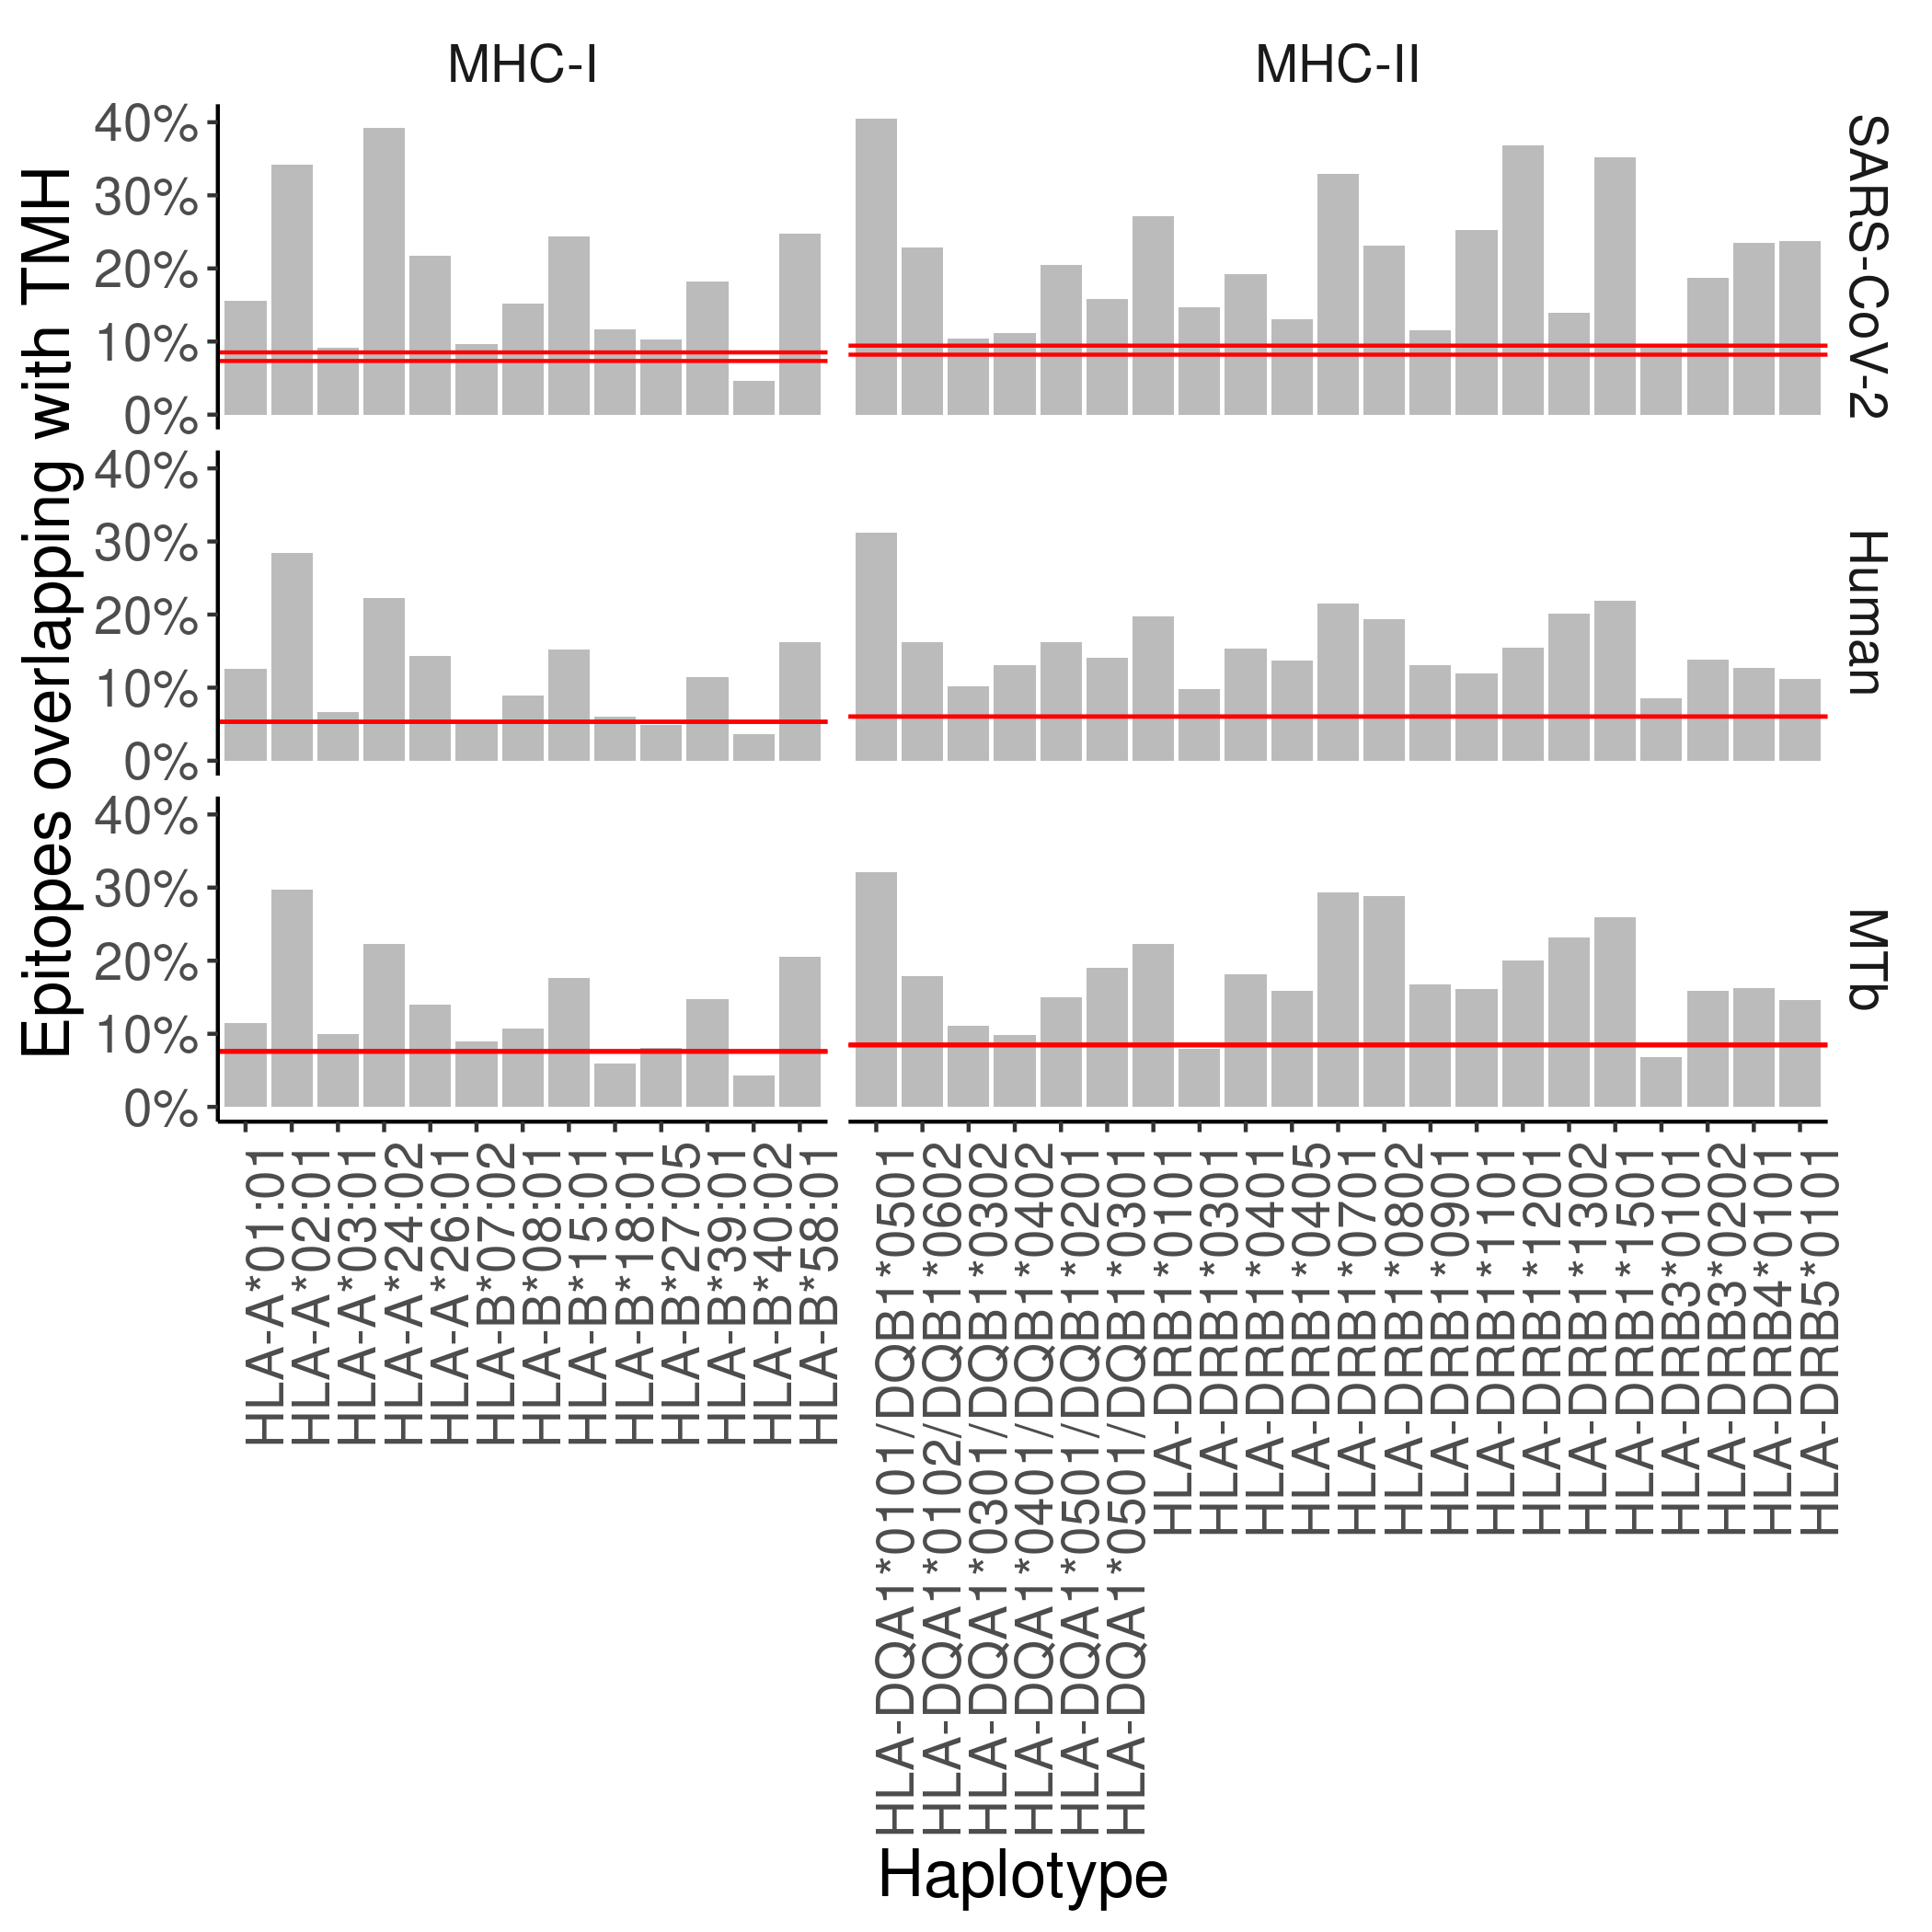
\includegraphics[width=\linewidth]{bbbq_1_smart_results/fig_f_tmh_2_panel.png}
    \label{fig:bbbq_1_smart_results}
  \end{subfigure}

  \vfill

  \begin{subfigure}[t]{0.35\textwidth}
    \centering
    \caption{}
    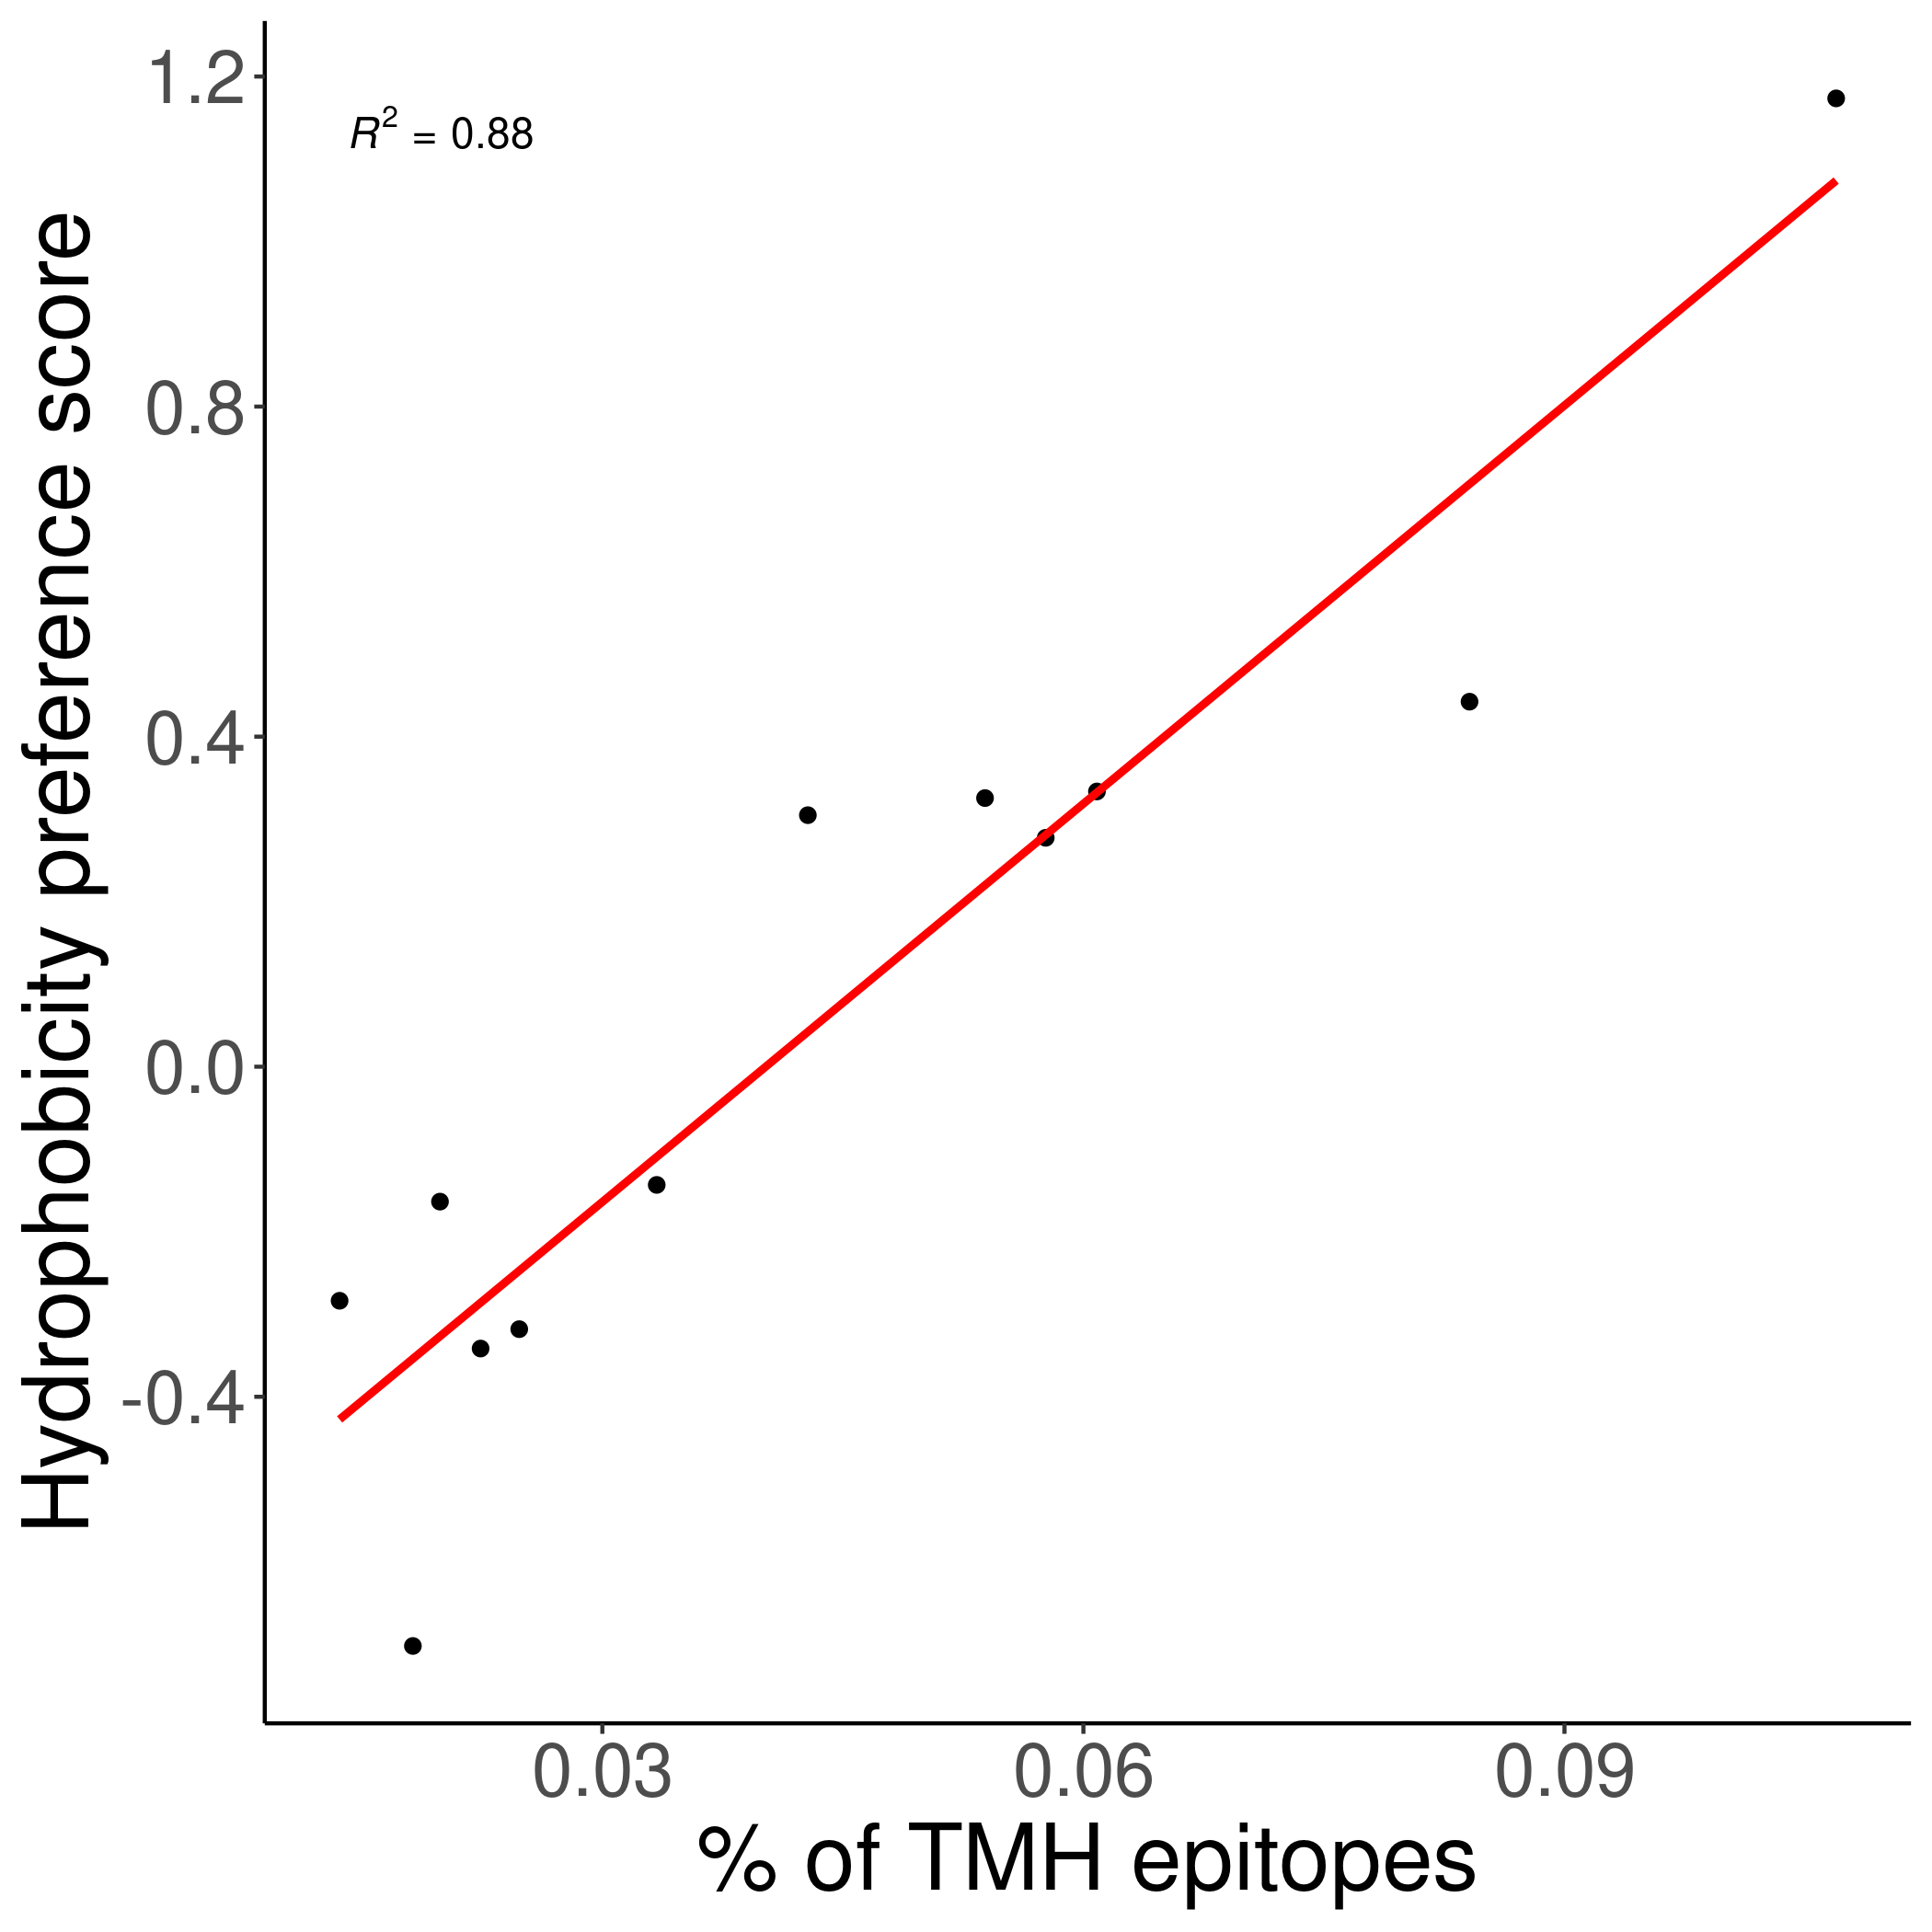
\includegraphics[width=\linewidth]{bbbq_1_smart_results/fig_hydrophobicity_mhc1.png}
    \label{fig:hydrophobicity_1}
  \end{subfigure}  
  \hfill
  \begin{subfigure}[t]{0.35\textwidth}
    \centering
    \caption{}
    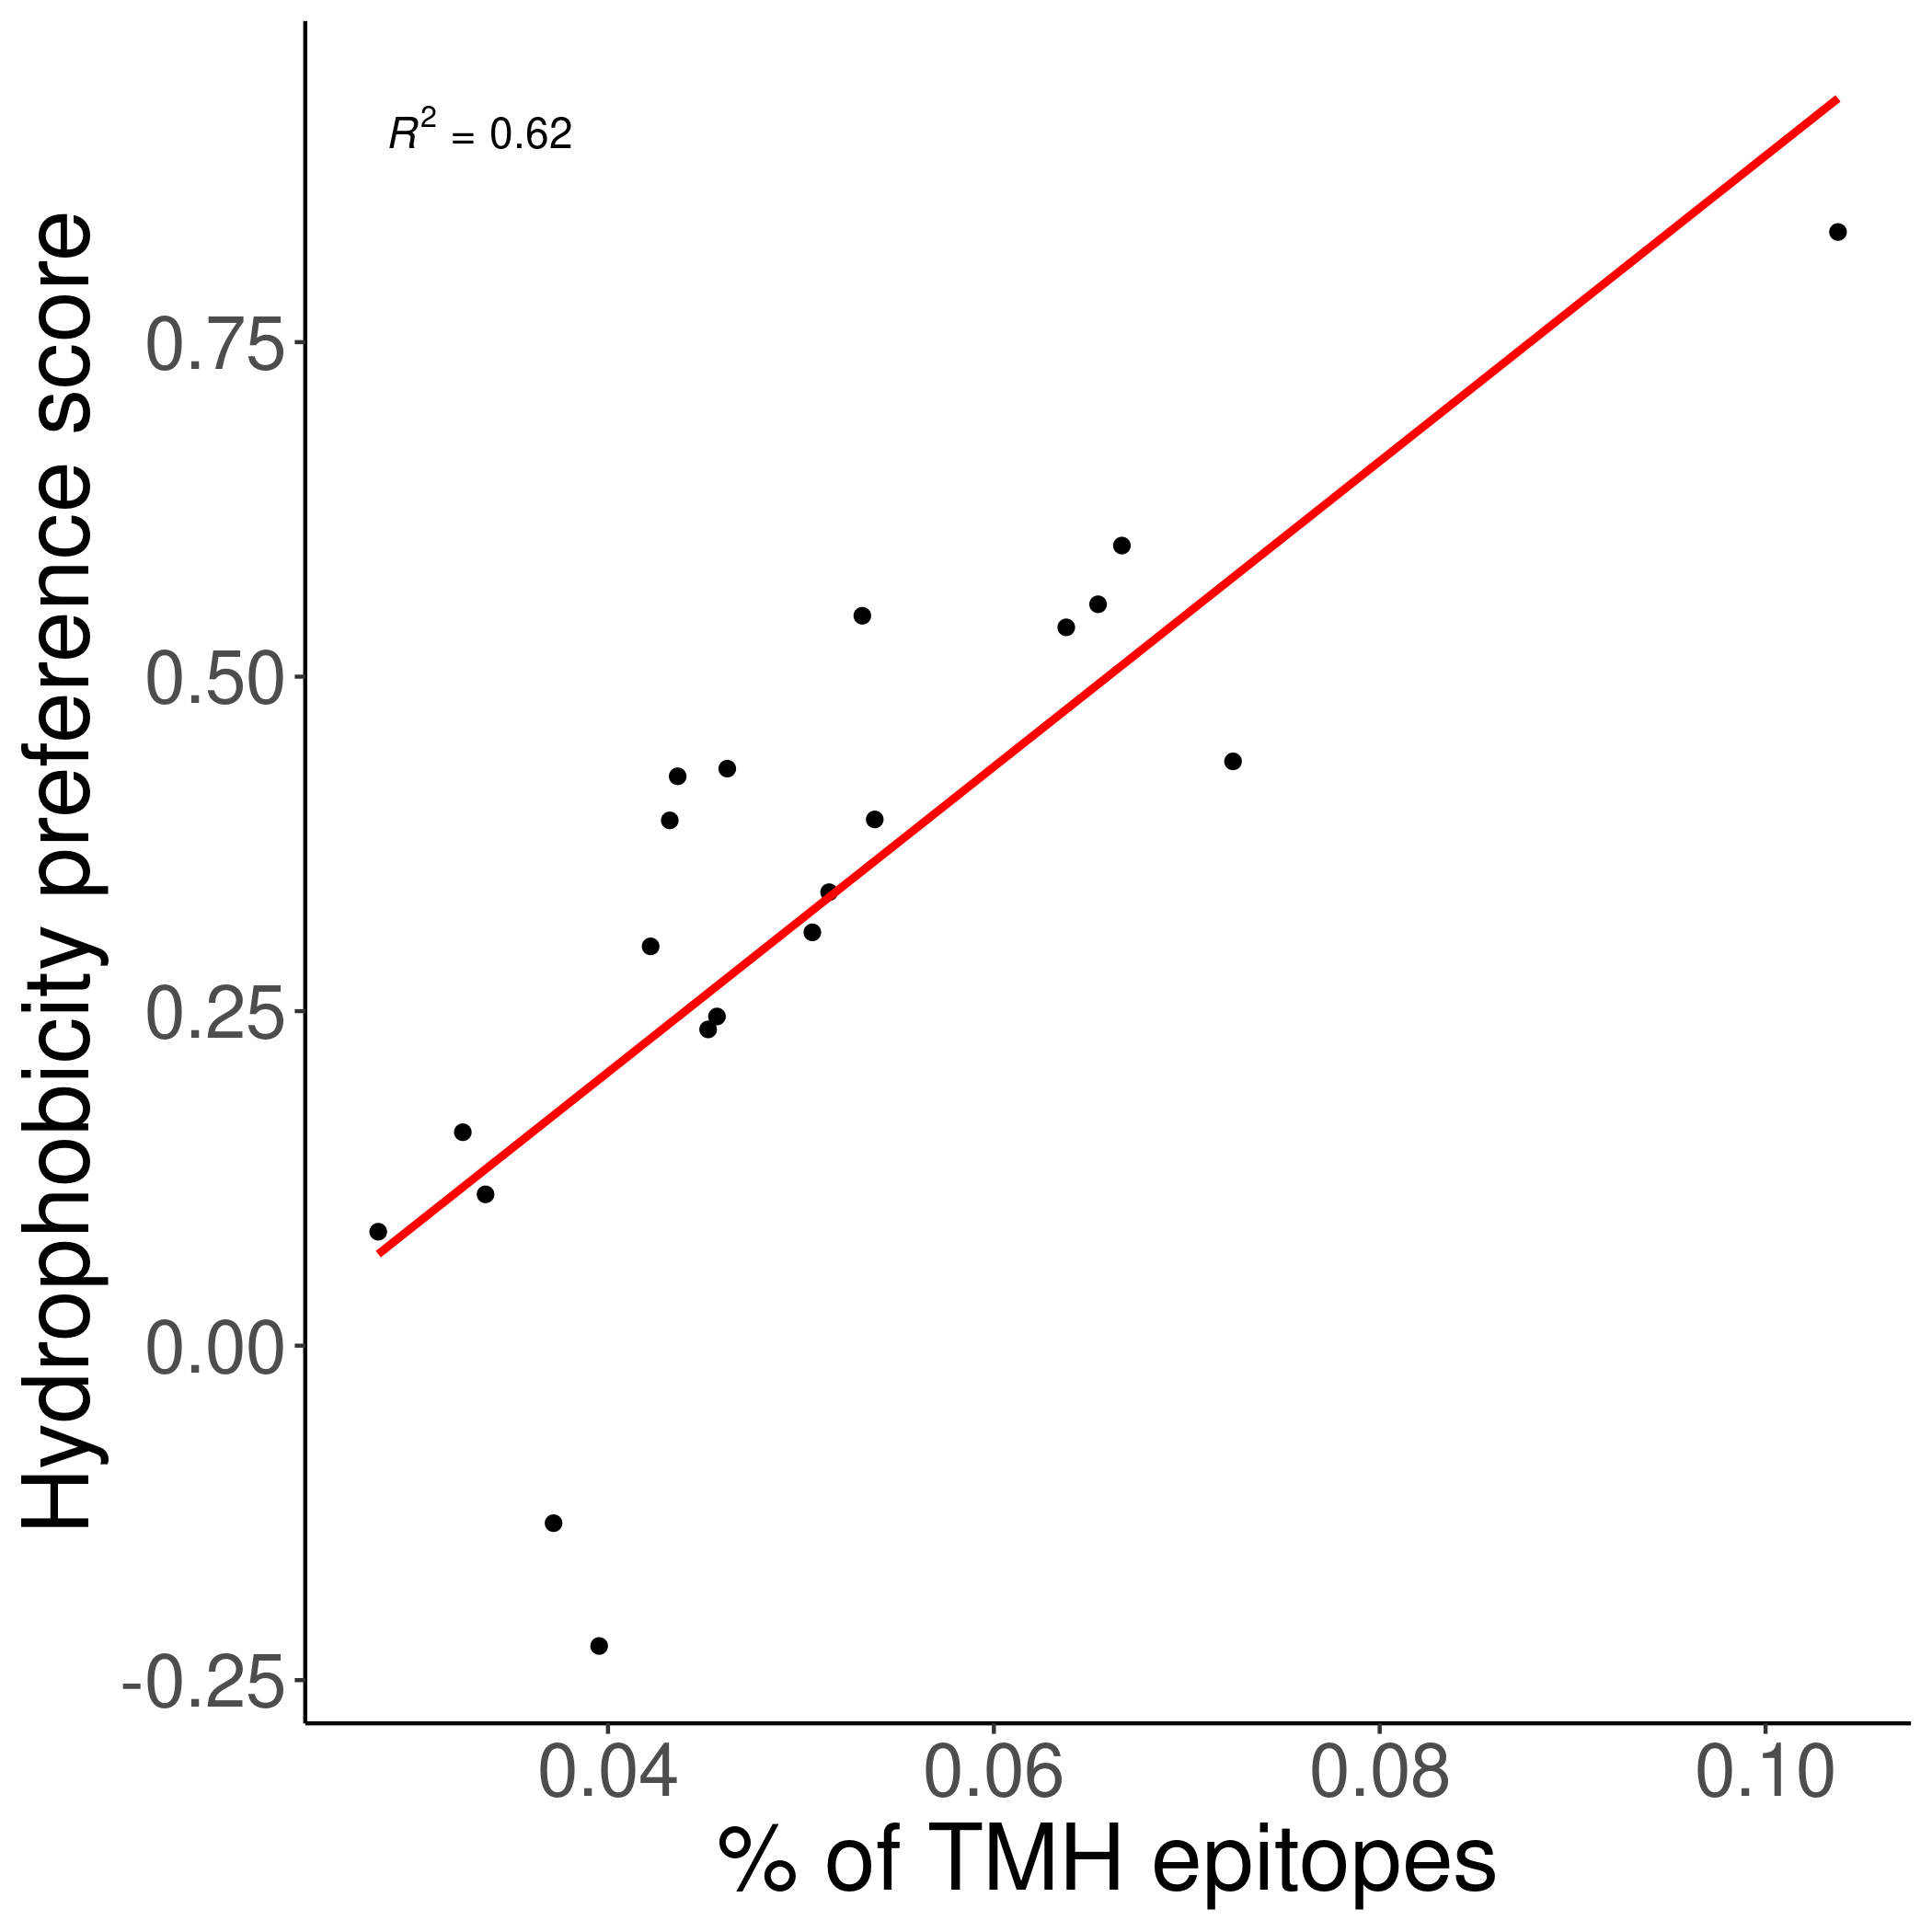
\includegraphics[width=\linewidth]{bbbq_1_smart_results/fig_hydrophobicity_mhc2.png}
    \label{fig:hydrophobicity_2}
  \end{subfigure}  
  \caption{ \textbf{Over-presentation of TMH-derived epitopes on most MHC-I and -II haplotypes}
    \textbf{(A)} 
    The percentage of epitopes for MHC-I and -II haplotypes that are predicted to 
    overlap with TMHs for the proteomes of SARS-CoV-2 (top row), human (middle 
    row) and \emph{M. tuberculosis} (MtB; bottom row).
    The pair of horizontal red lines in each plot indicate the lower and upper bound 
    of the 99\% confidence interval.
    See supplementary Tables \ref{tab:tmh_binders_mhc2} and \ref{tab:tmh_binders_mhc1}
    for the exact TMH and  epitope counts.
    \textbf{(B-C)}
    Correlation between the percentages of predicted TMH-derived epitopes
    and the hydrophobicity score of all predicted epitopes for 
    human MHC-I \textbf{(B)} and MHC-II alleles \textbf{(C)}.
    Diagonal red line: linear regression analysis. 
    Labels are shorthand for the HLA haplotypes,
    see the supplementary Table \ref{tab:haplotype_abbreviations} for the names.
  }
\end{figure}


% Process all floats before going to a next page
\clearpage

% No page number on this page
\thispagestyle{empty}

%
% Figure 2
%
\begin{figure}[!htbp]
  \centering
  \begin{subfigure}[t]{0.45\textwidth}
    \centering
    \caption{}
    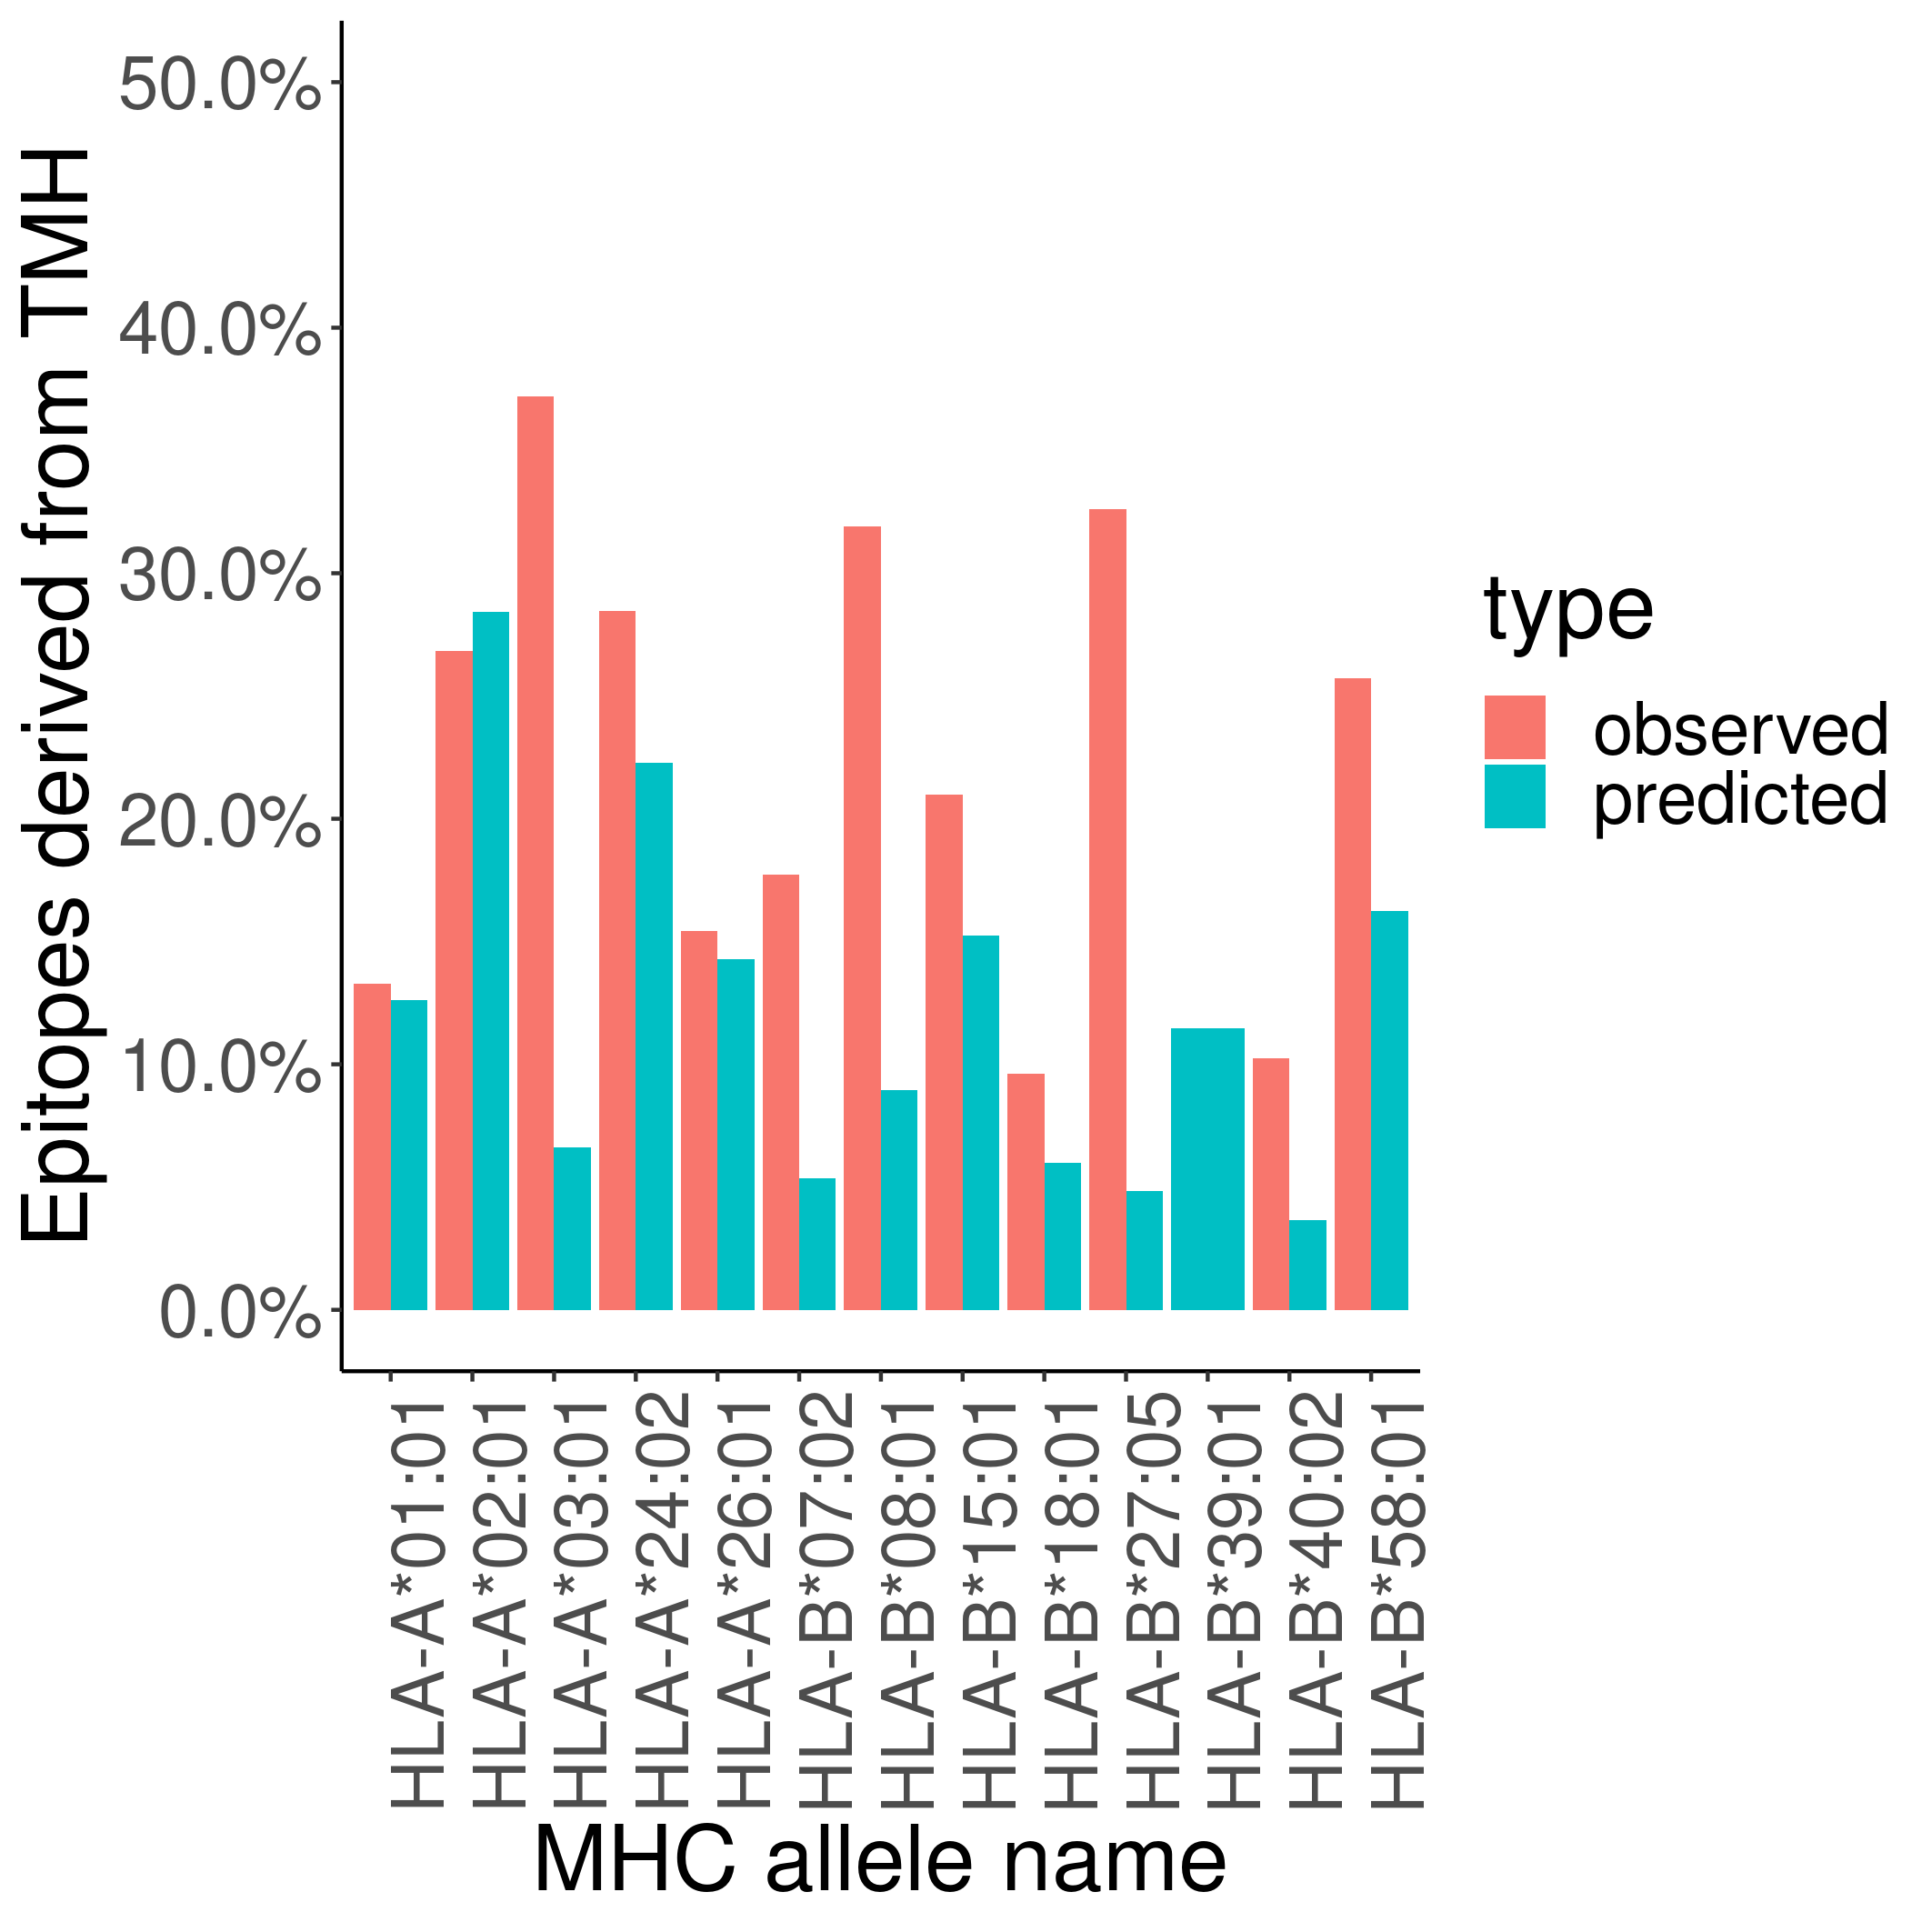
\includegraphics[width=1.0\textwidth]{bbbq_article_issue_157/figure_2a.png}
    \label{fig:2a}
  \end{subfigure}  
  \hfill
  \begin{subfigure}[t]{0.45\textwidth}
    \centering
    \caption{}
    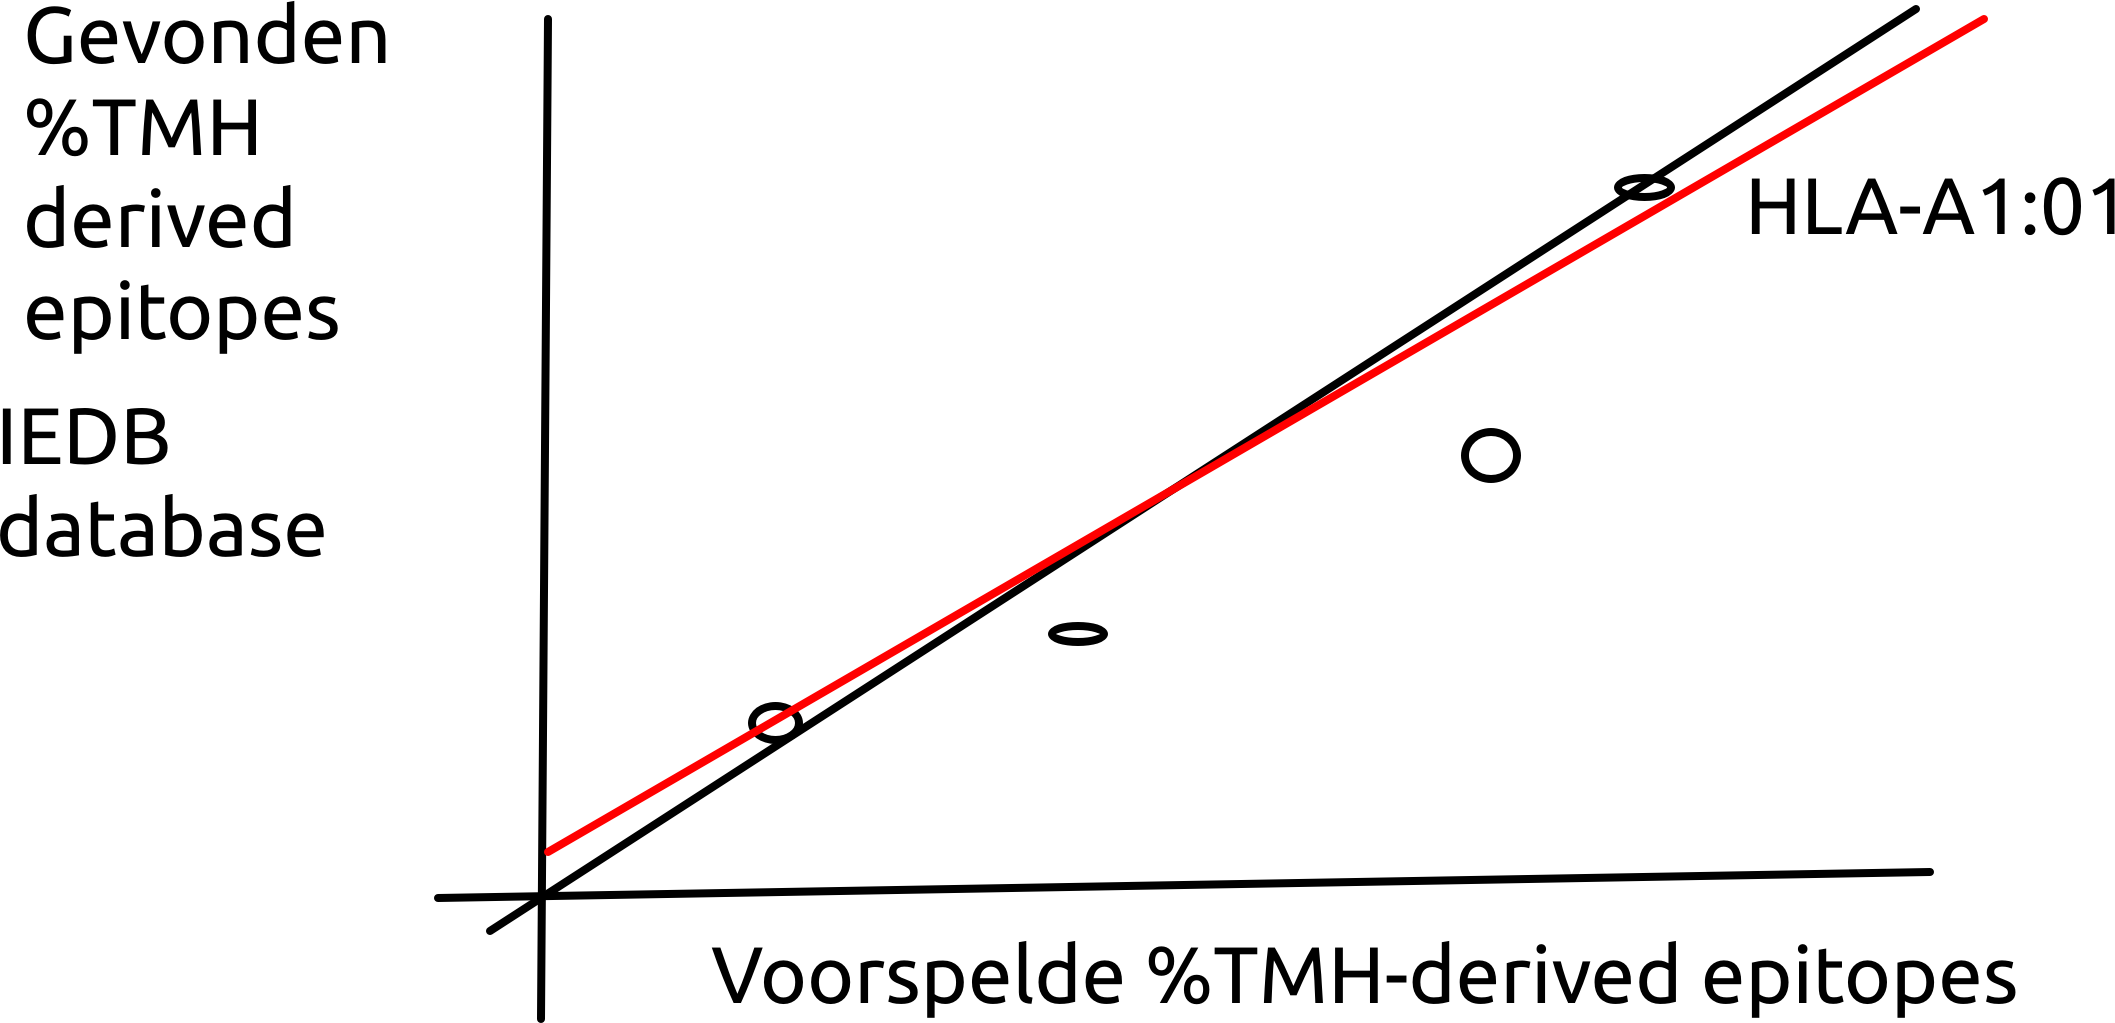
\includegraphics[width=1.0\textwidth]{bbbq_article_issue_157/figure_2b.png}
    \label{fig:2b}
  \end{subfigure}  

  \caption{
    \textbf{
      Robust prediction that TMH epitopes are presented \emph{in vivo}.
    }
    The percentage of epitopes for MHC-I and -II alleles
    that overlap with TMHs that are presented.
    The pair of horizontal red lines in each plot indicate the lower and upper bound 
    of the 99\% confidence interval. Note that only one line is visible as this
    interval is relatively narrow.
    Alleles are listed in Table \ref{tab:haplotype_abbreviations}).
    \textbf{(A)} 
    Observed and predicted percentage of TMH-derived epitopes
    \textbf{(B)} 
    MHC ligands from IEDB binding to TMH-derived epitopes.
    The numbers above the bars denotes the number of epitopes
    obtained using an MHC ligand assay. 
  }
  \label{fig:elution}
\end{figure}

% Process all floats before going to a next page
\clearpage

% No page number on this page
\thispagestyle{empty}

%
% Figure 3
%
\begin{figure}[!htbp]
  \centering

  \begin{subfigure}[t]{0.45\textwidth}
    \centering
    \caption{}
    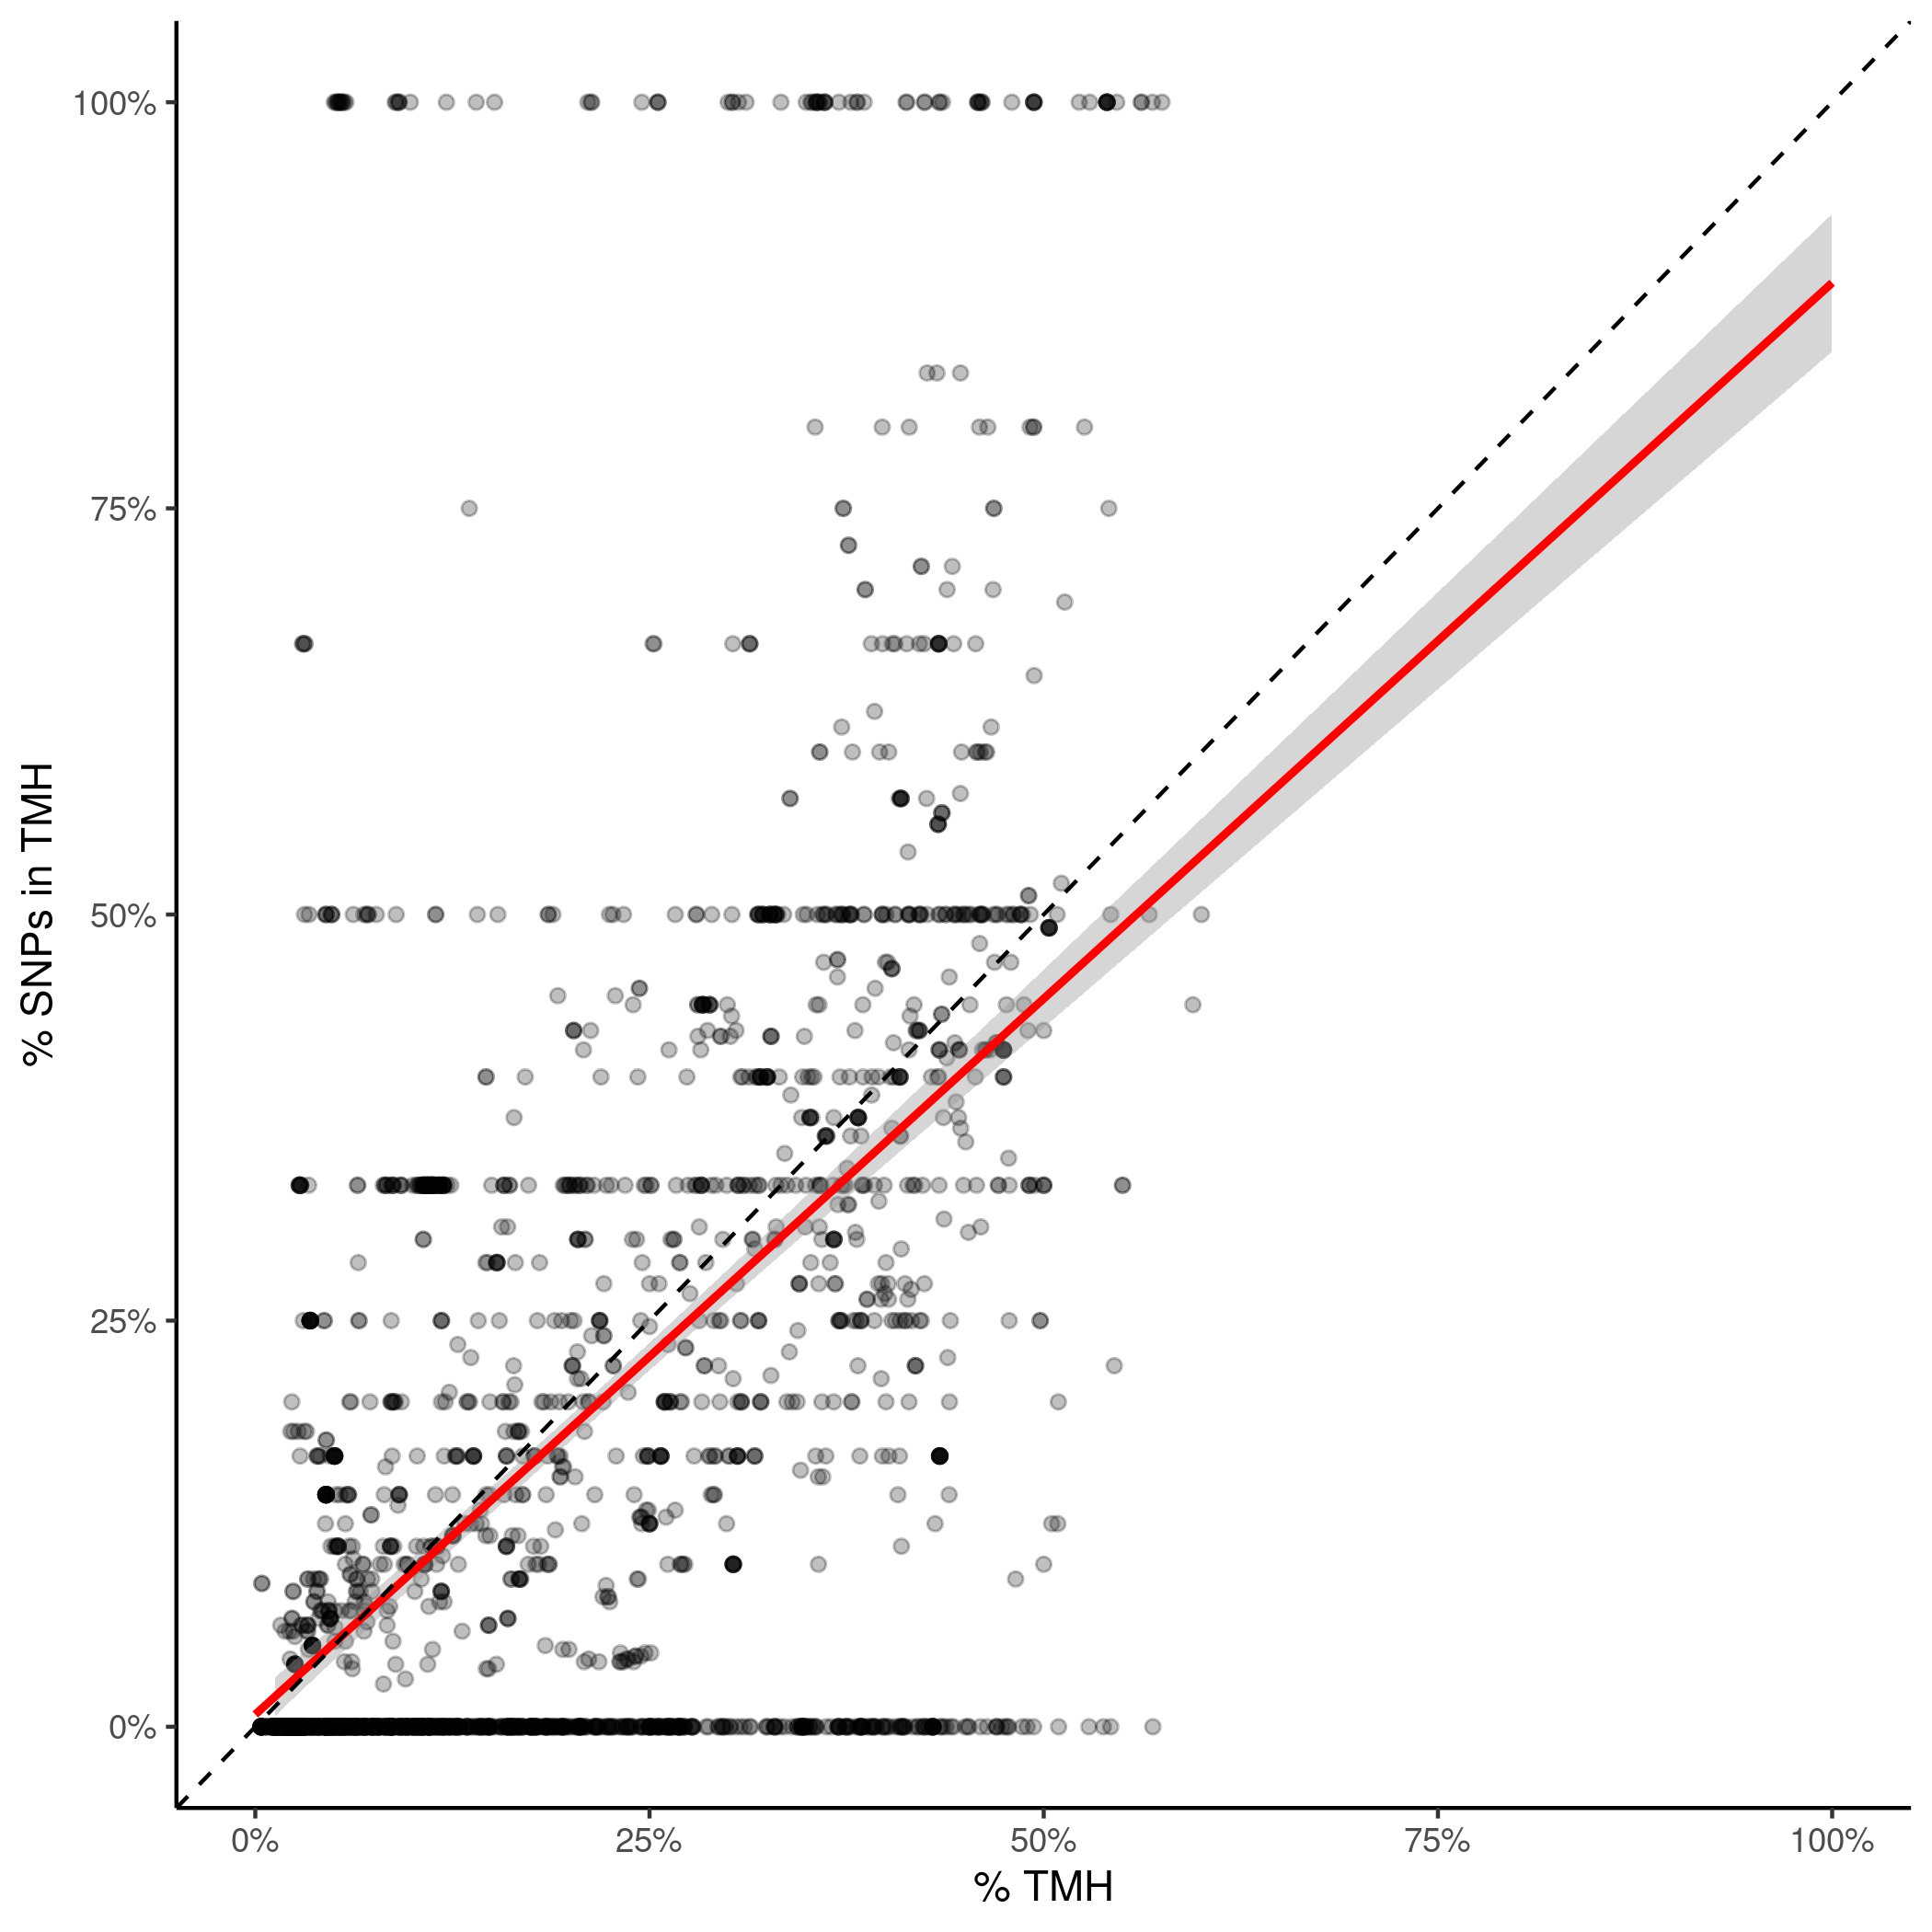
\includegraphics[width=\linewidth]{ncbi_peregrine_results/fig_f_snps_found_and_expected.png}
    \label{fig:f_snps_found_and_expected}
  \end{subfigure}
  \hfill
  \begin{subfigure}[t]{0.45\textwidth}
    \centering
    \caption{}
    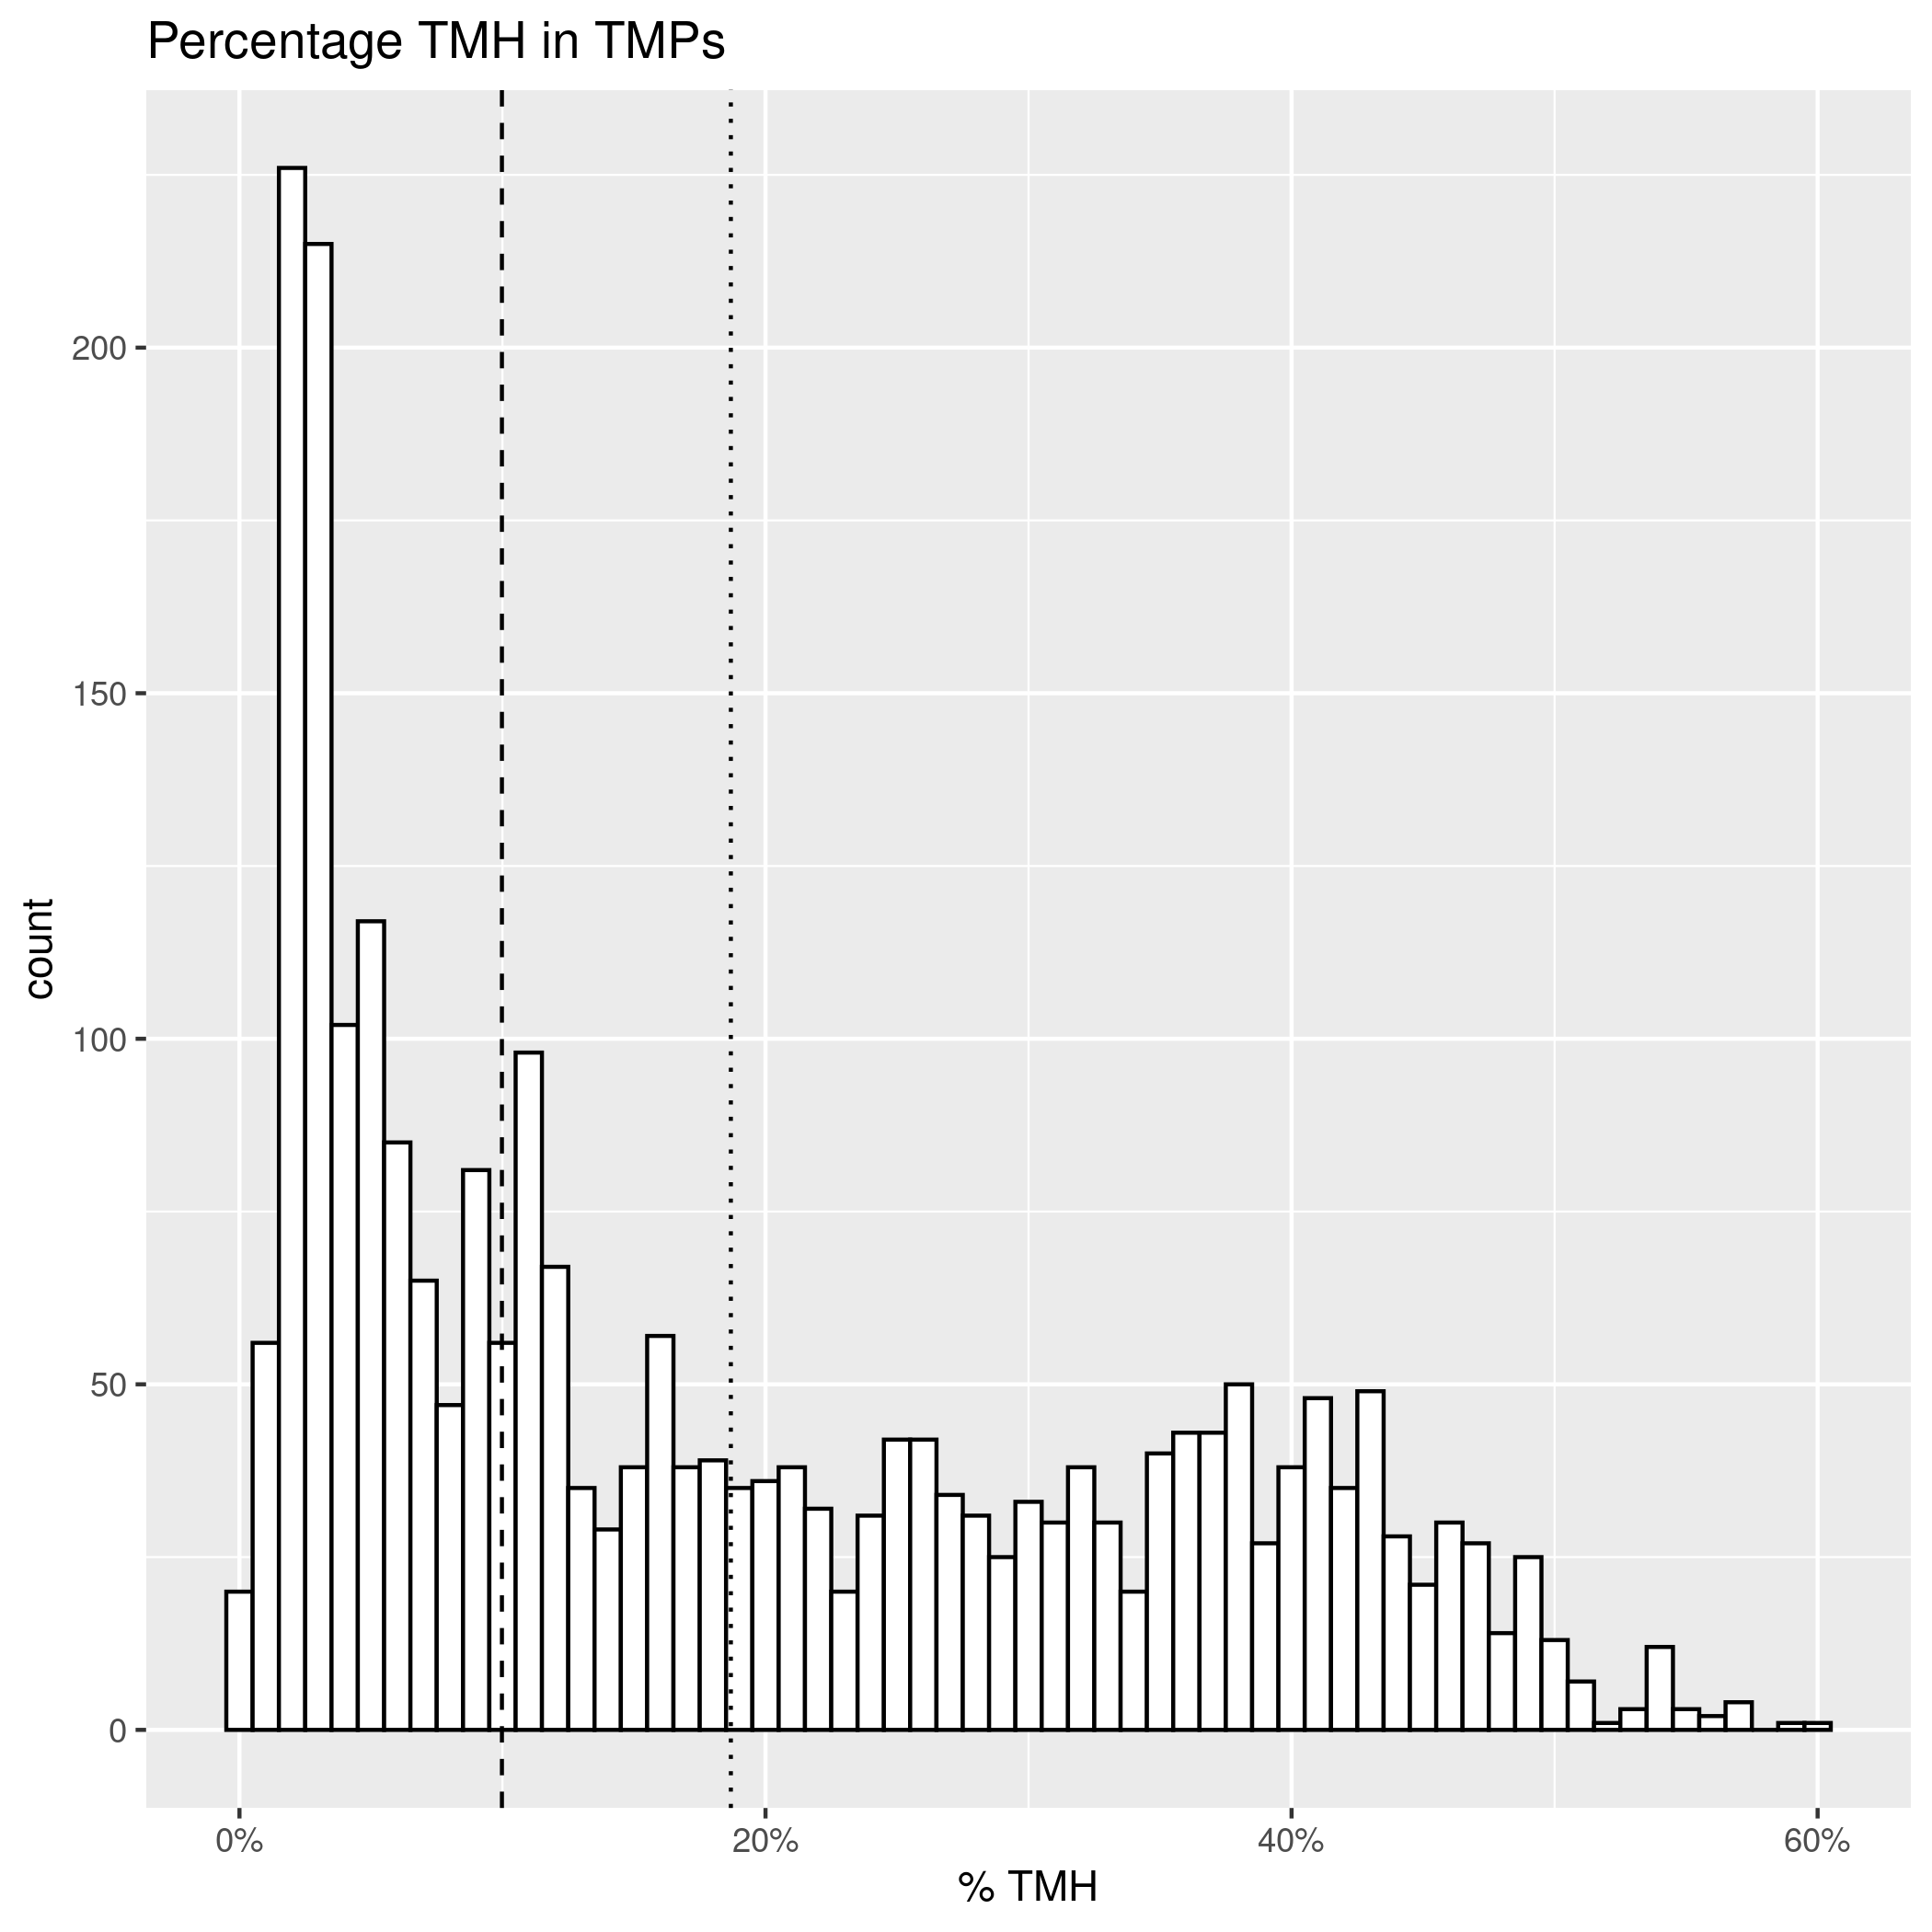
\includegraphics[width=\linewidth]{ncbi_peregrine_results/fig_f_tmh_ncbi.png}
    \label{fig:f_tmh_ncbi}
  \end{subfigure}  

  
   \vfill

  \begin{subfigure}[t]{0.45\textwidth}
    \centering
    \caption{}
    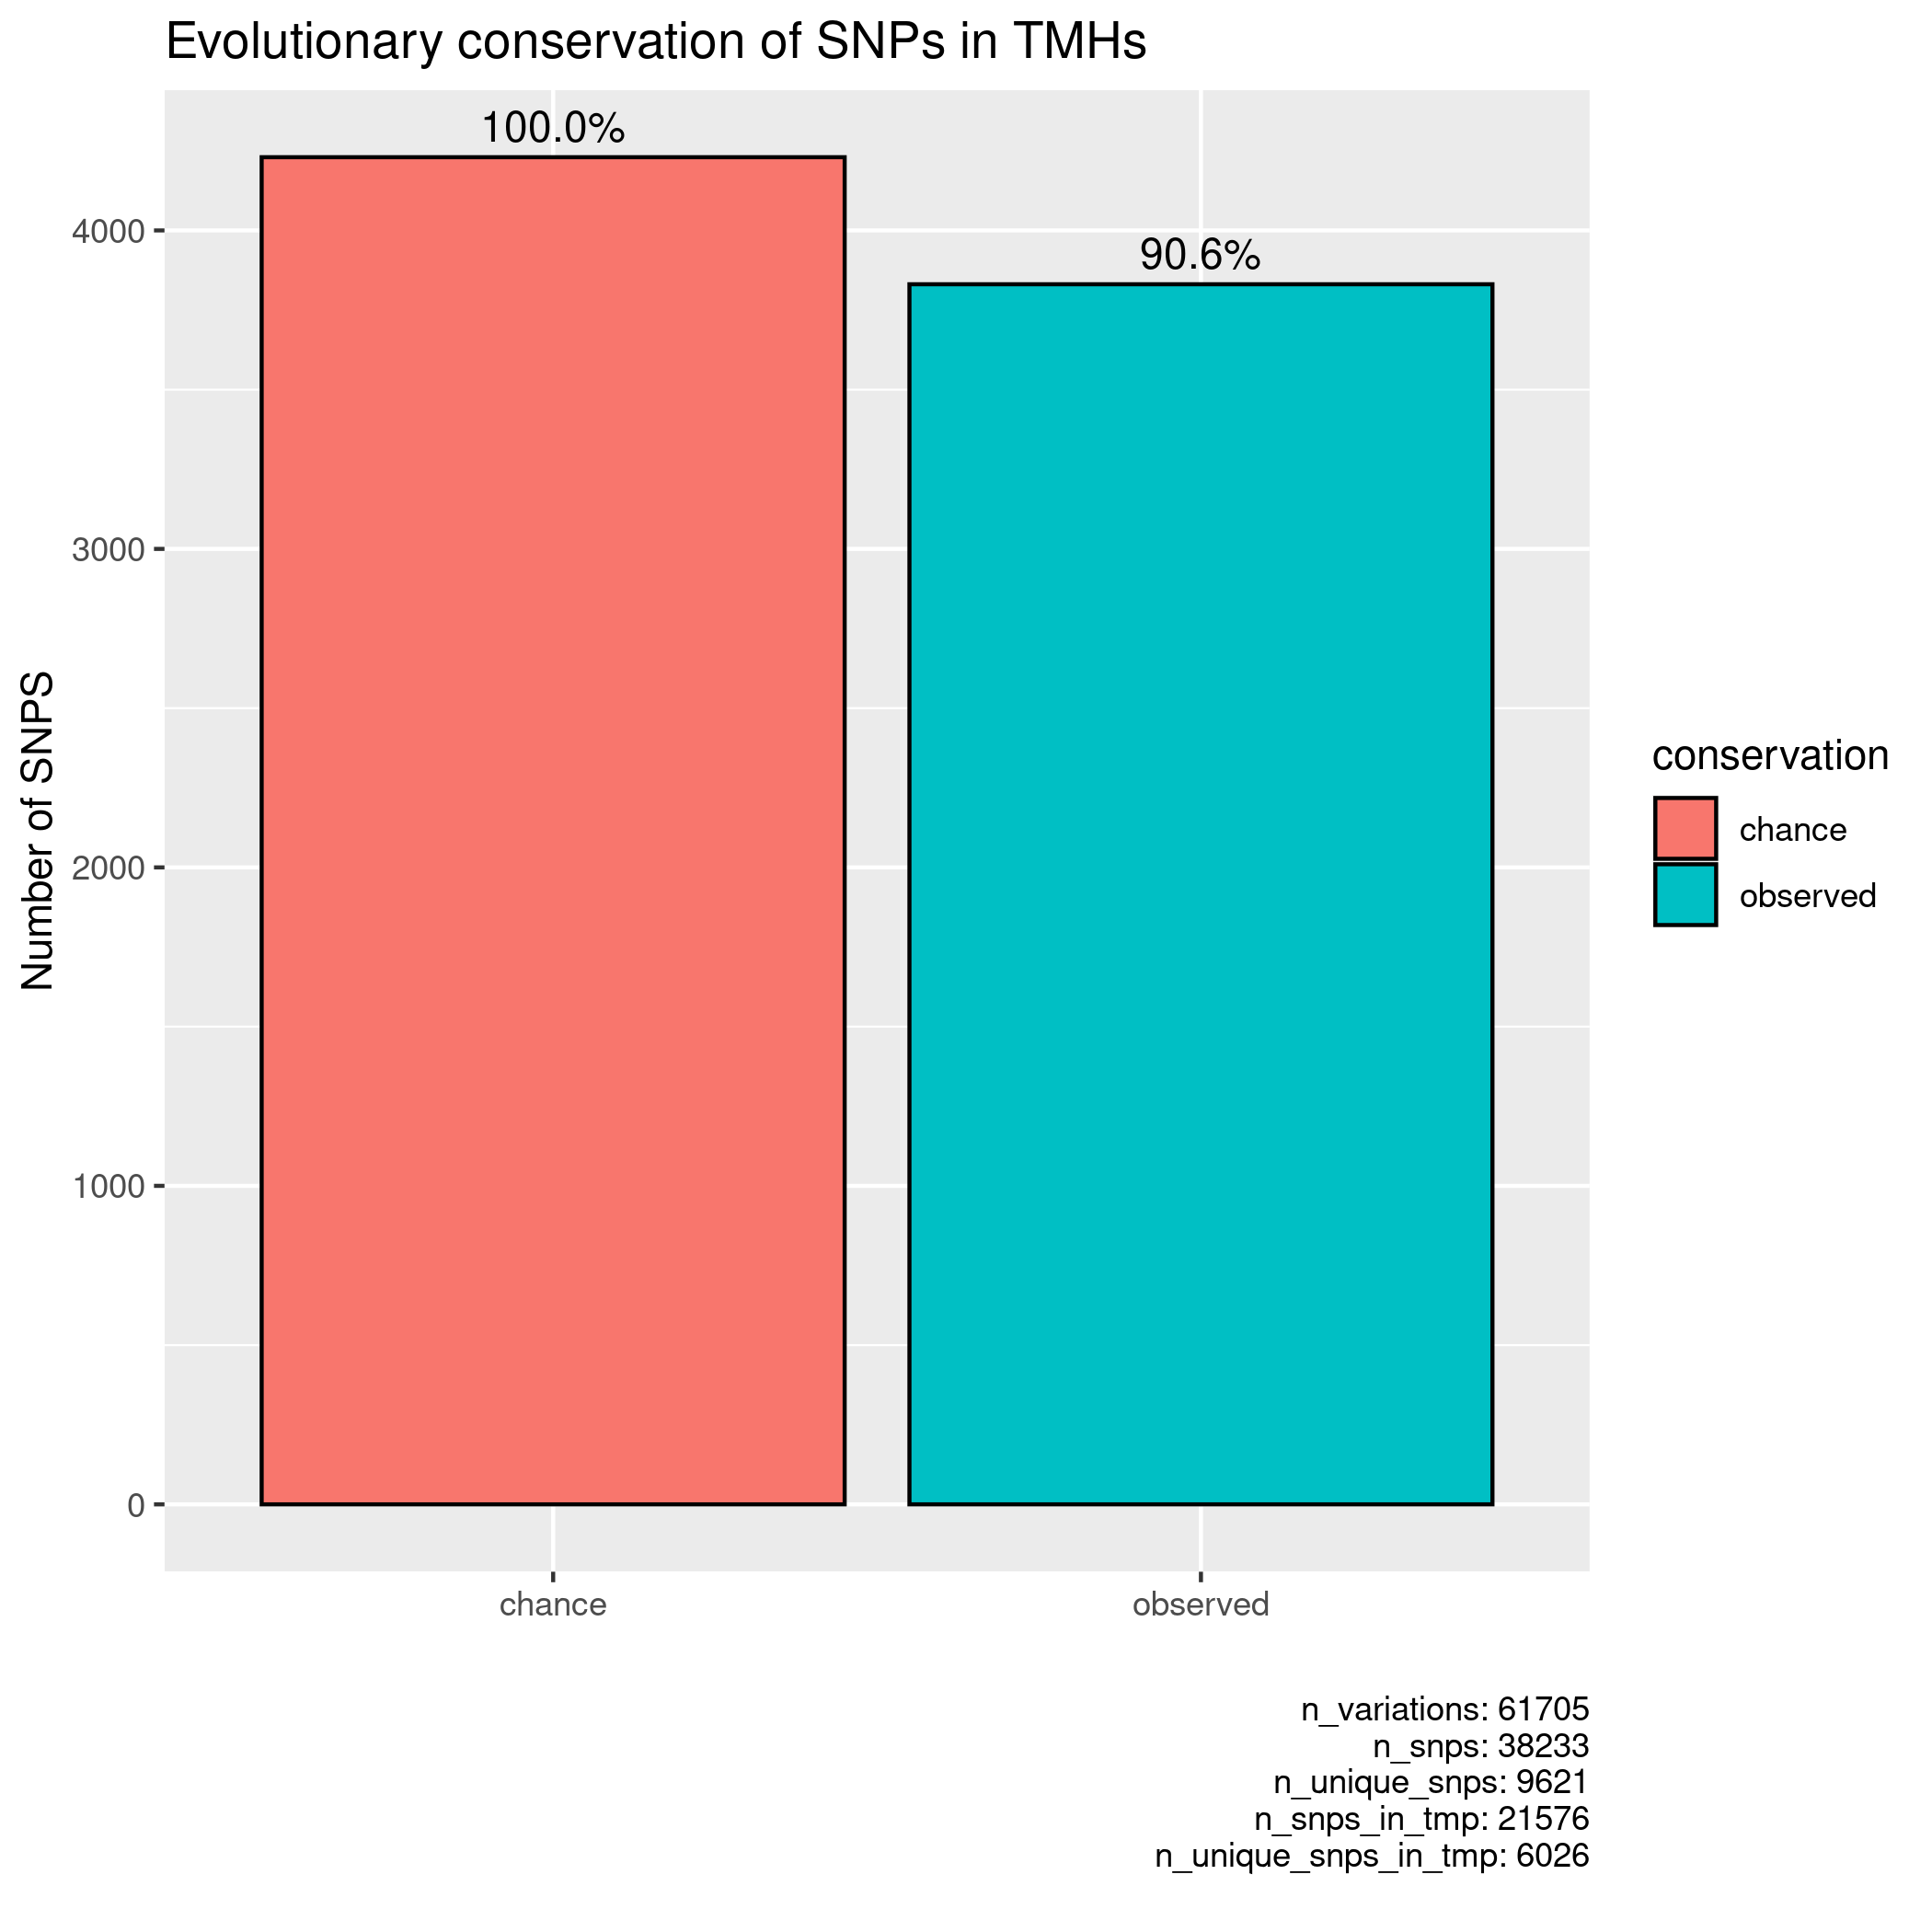
\includegraphics[width=\linewidth]{ncbi_peregrine_results/fig_conservation.png}
    \label{fig:conservation}
  \end{subfigure}


  \caption{ \textbf{Evolutionary conservation of human TMHs.}
    \textbf{(A)} 
    Percentage of SNPs found in TMHs.
    Each point shows for one protein the predicted percentage of
    amino acids that are part of a TMH ($x$-axis) and the observed occurrence of SNPs being located
    within a TMH ($y$-axis).
    The dashed diagonal line shows the line of equality (i.e.,
    equal conservation of TMHs and soluble protein regions). 
    The diagonal red line indicates a linear fit, 
    the gray area its 95\% confidence interval.
    \textbf{(B)}
    Distribution of the percentages of TMH in the TMPs used in this study.
    \textbf{(C)}
    The number of SNPs in TMHs as expected by chance (left bar) 
    and found in the dbSNP database (right bar).
    Percentages show the relative conservation
    of SNPs in TMHs found relative to stochastic chance.
  }
\end{figure}

% Process all floats before going to a next page
\clearpage

% No page number on this page
\thispagestyle{empty}

%
% Figure 4
%
\begin{figure}[!htbp]
  \centering

  \begin{subfigure}[t]{\textwidth}
    \centering
    \caption{}
    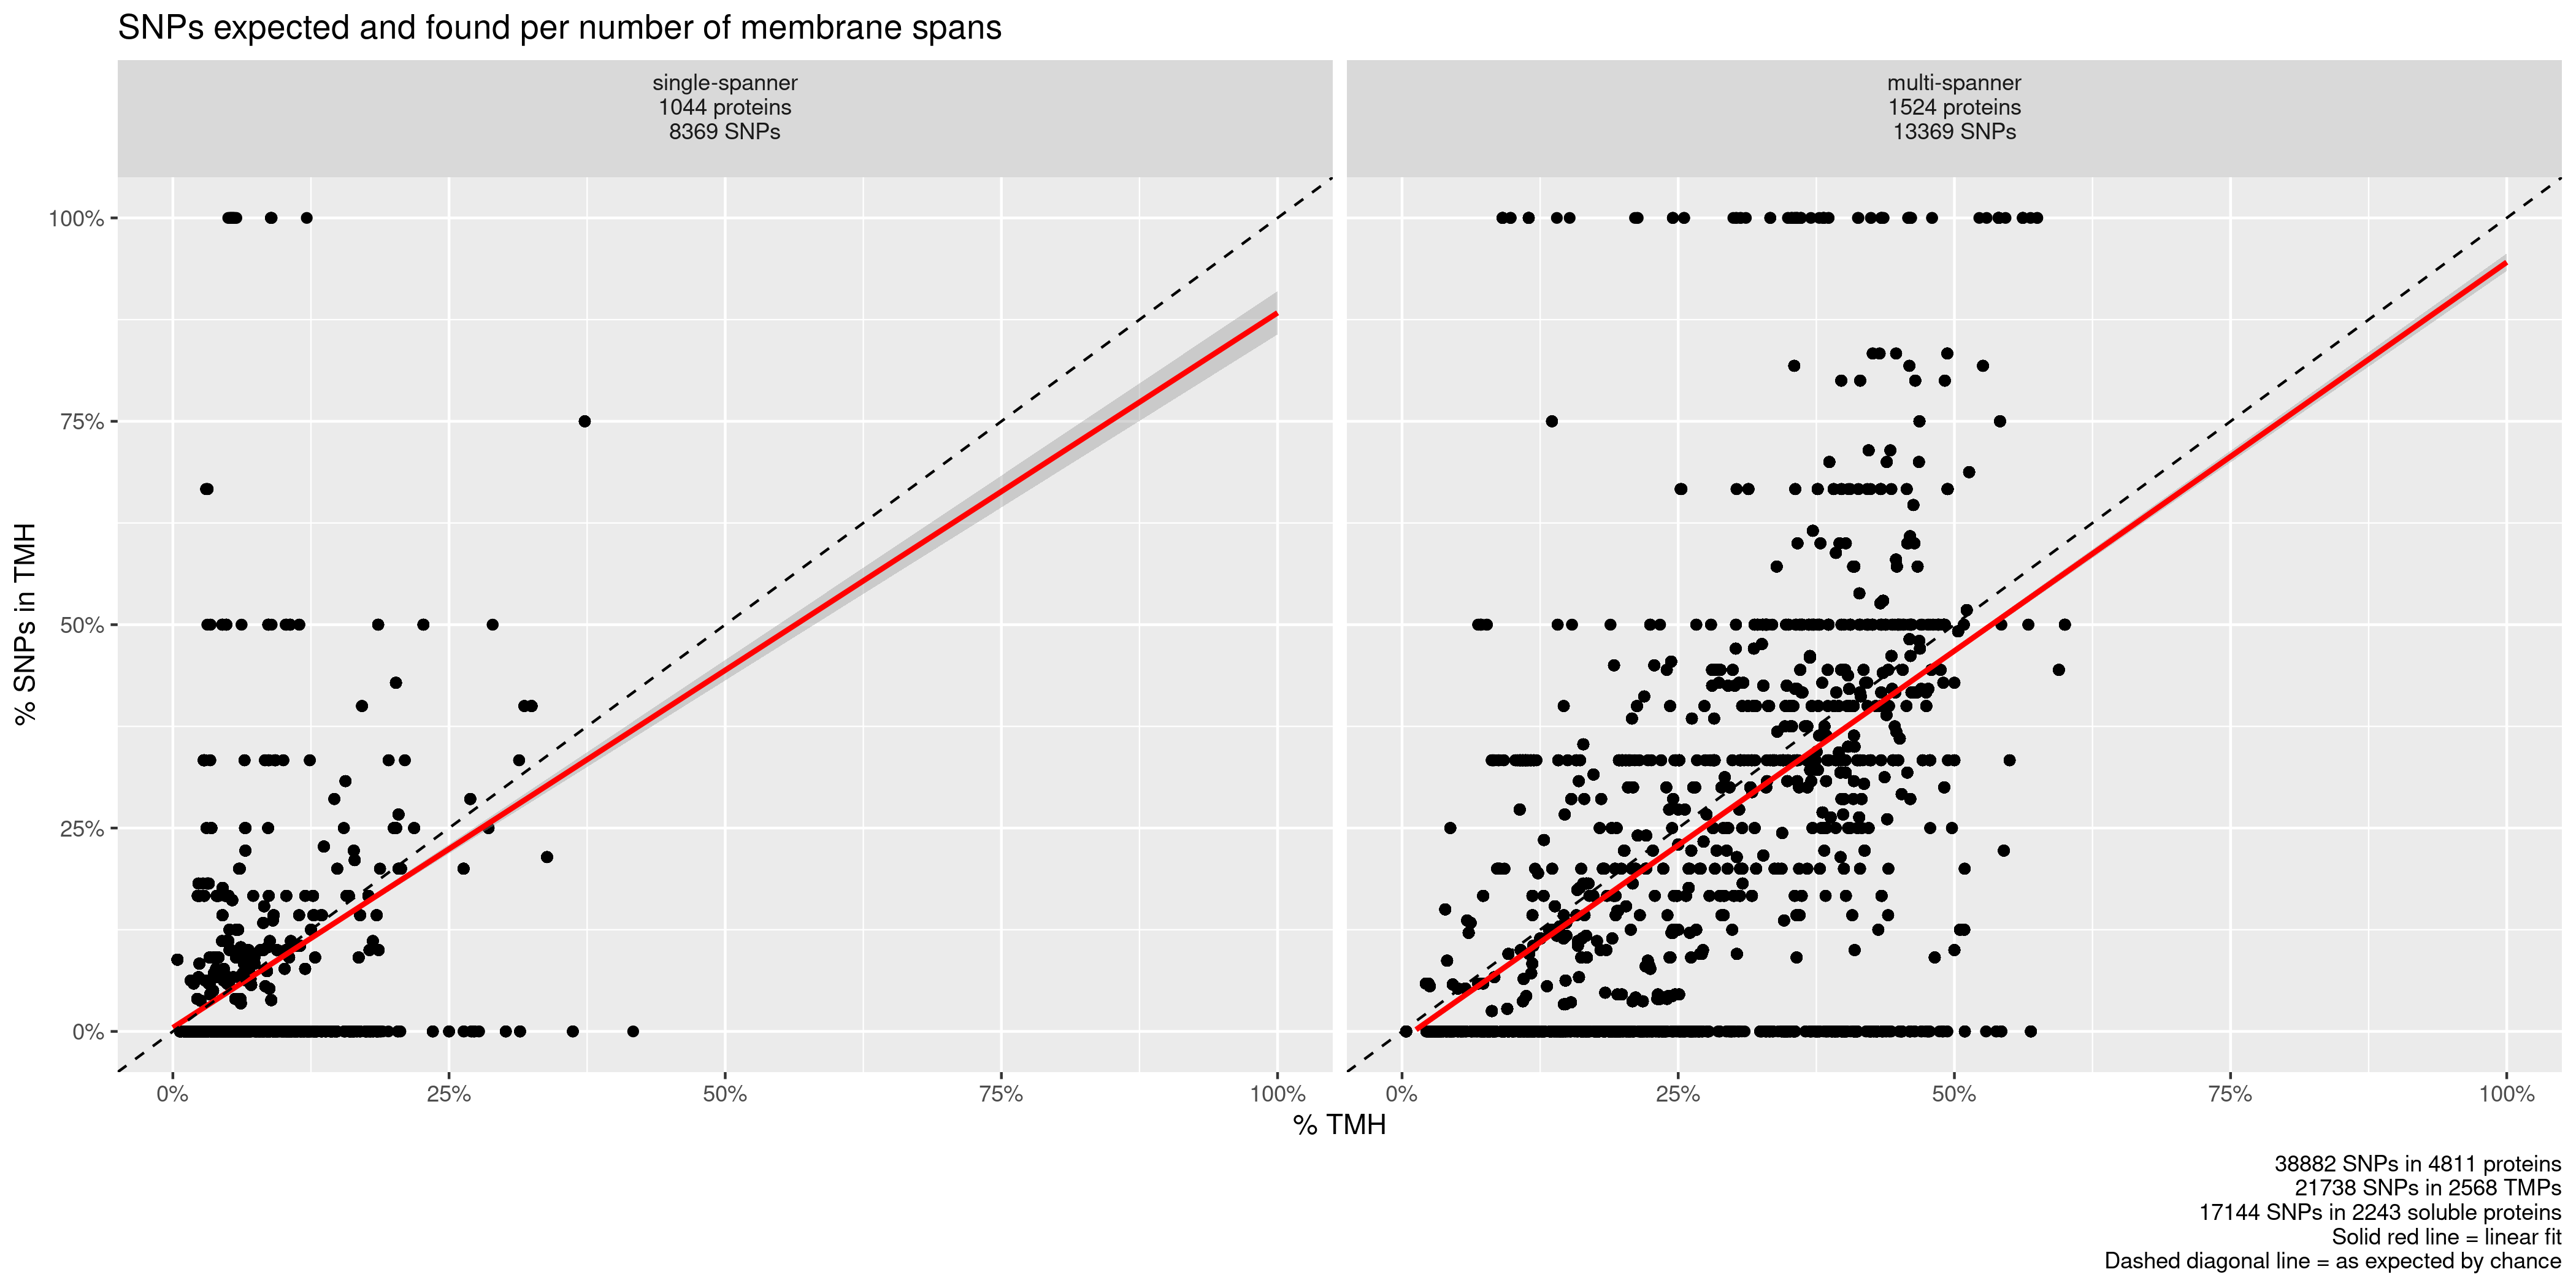
\includegraphics[width=\linewidth]{ncbi_peregrine_results/fig_f_snps_found_and_expected_per_spanner.png}
    \label{fig:f_snps_found_and_expected_per_spanner}
  \end{subfigure}

  \vfill

  \begin{subfigure}[t]{0.45\textwidth}
    \centering
    \caption{}
    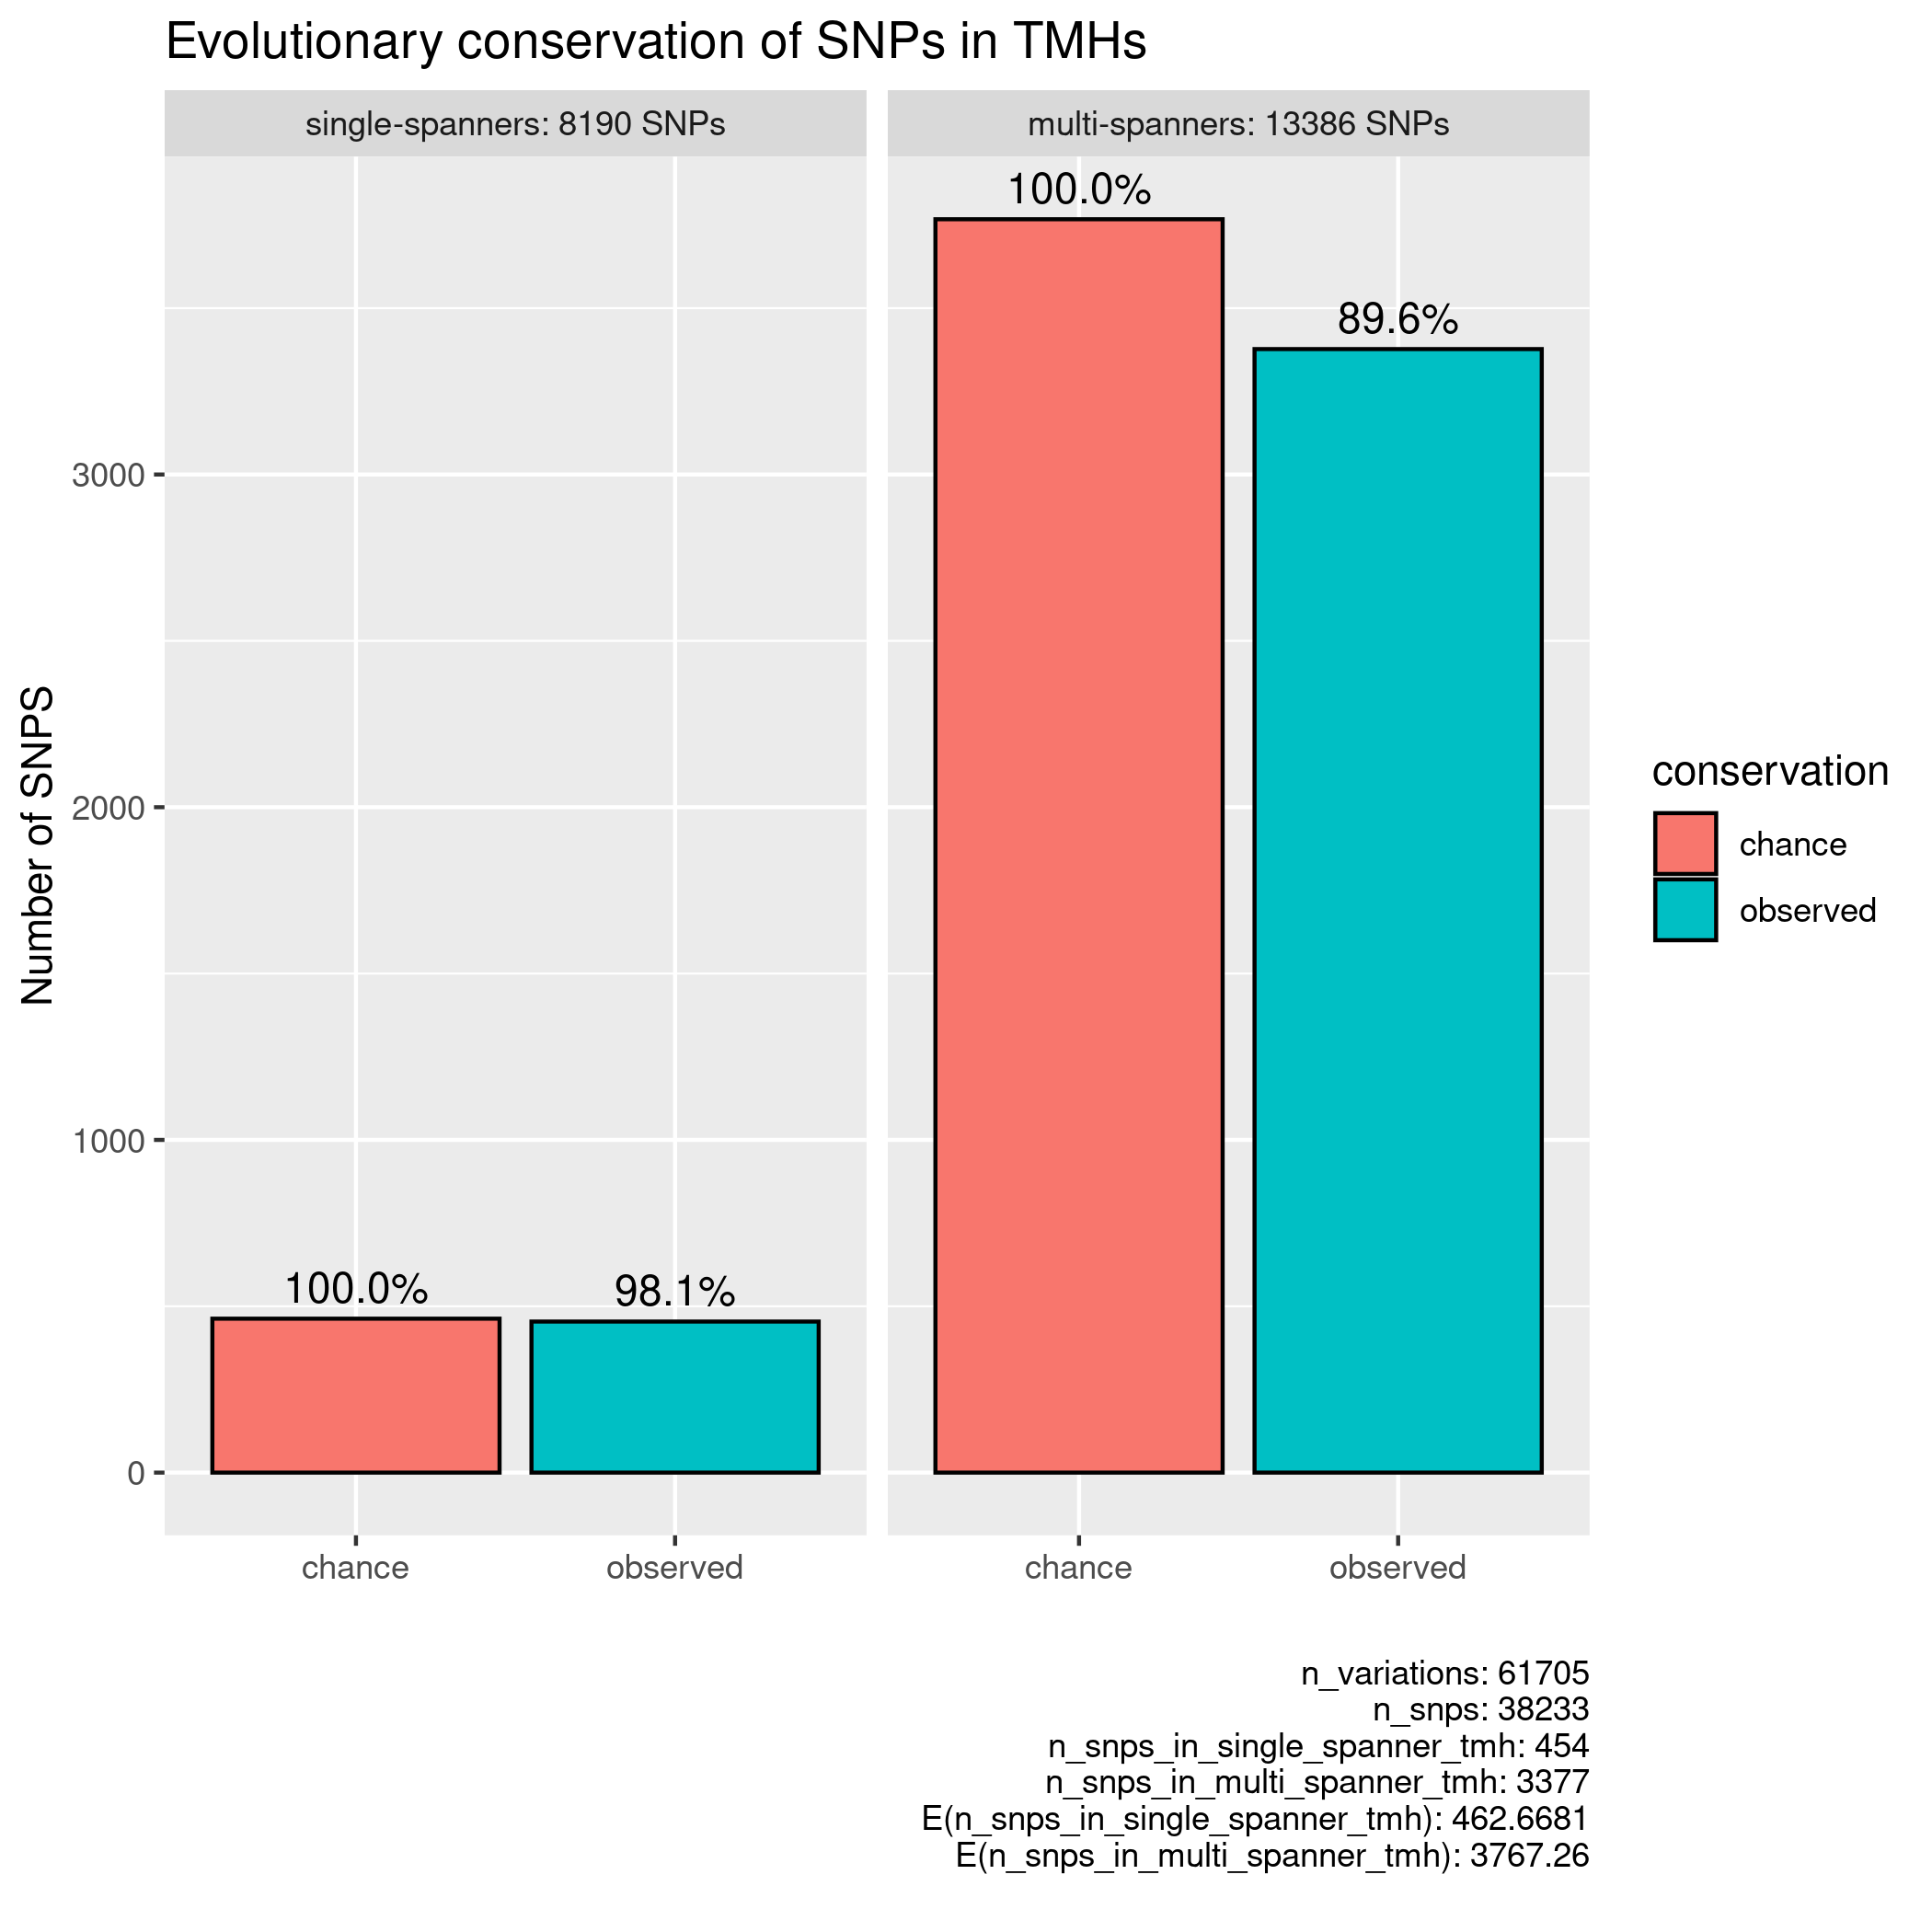
\includegraphics[width=\linewidth]{ncbi_peregrine_results/fig_conservation_per_spanner.png}
    \label{fig:conservation_per_spanner}
  \end{subfigure}
  \hfill
  \begin{subfigure}[t]{0.45\textwidth}
    \centering
    \caption{}
    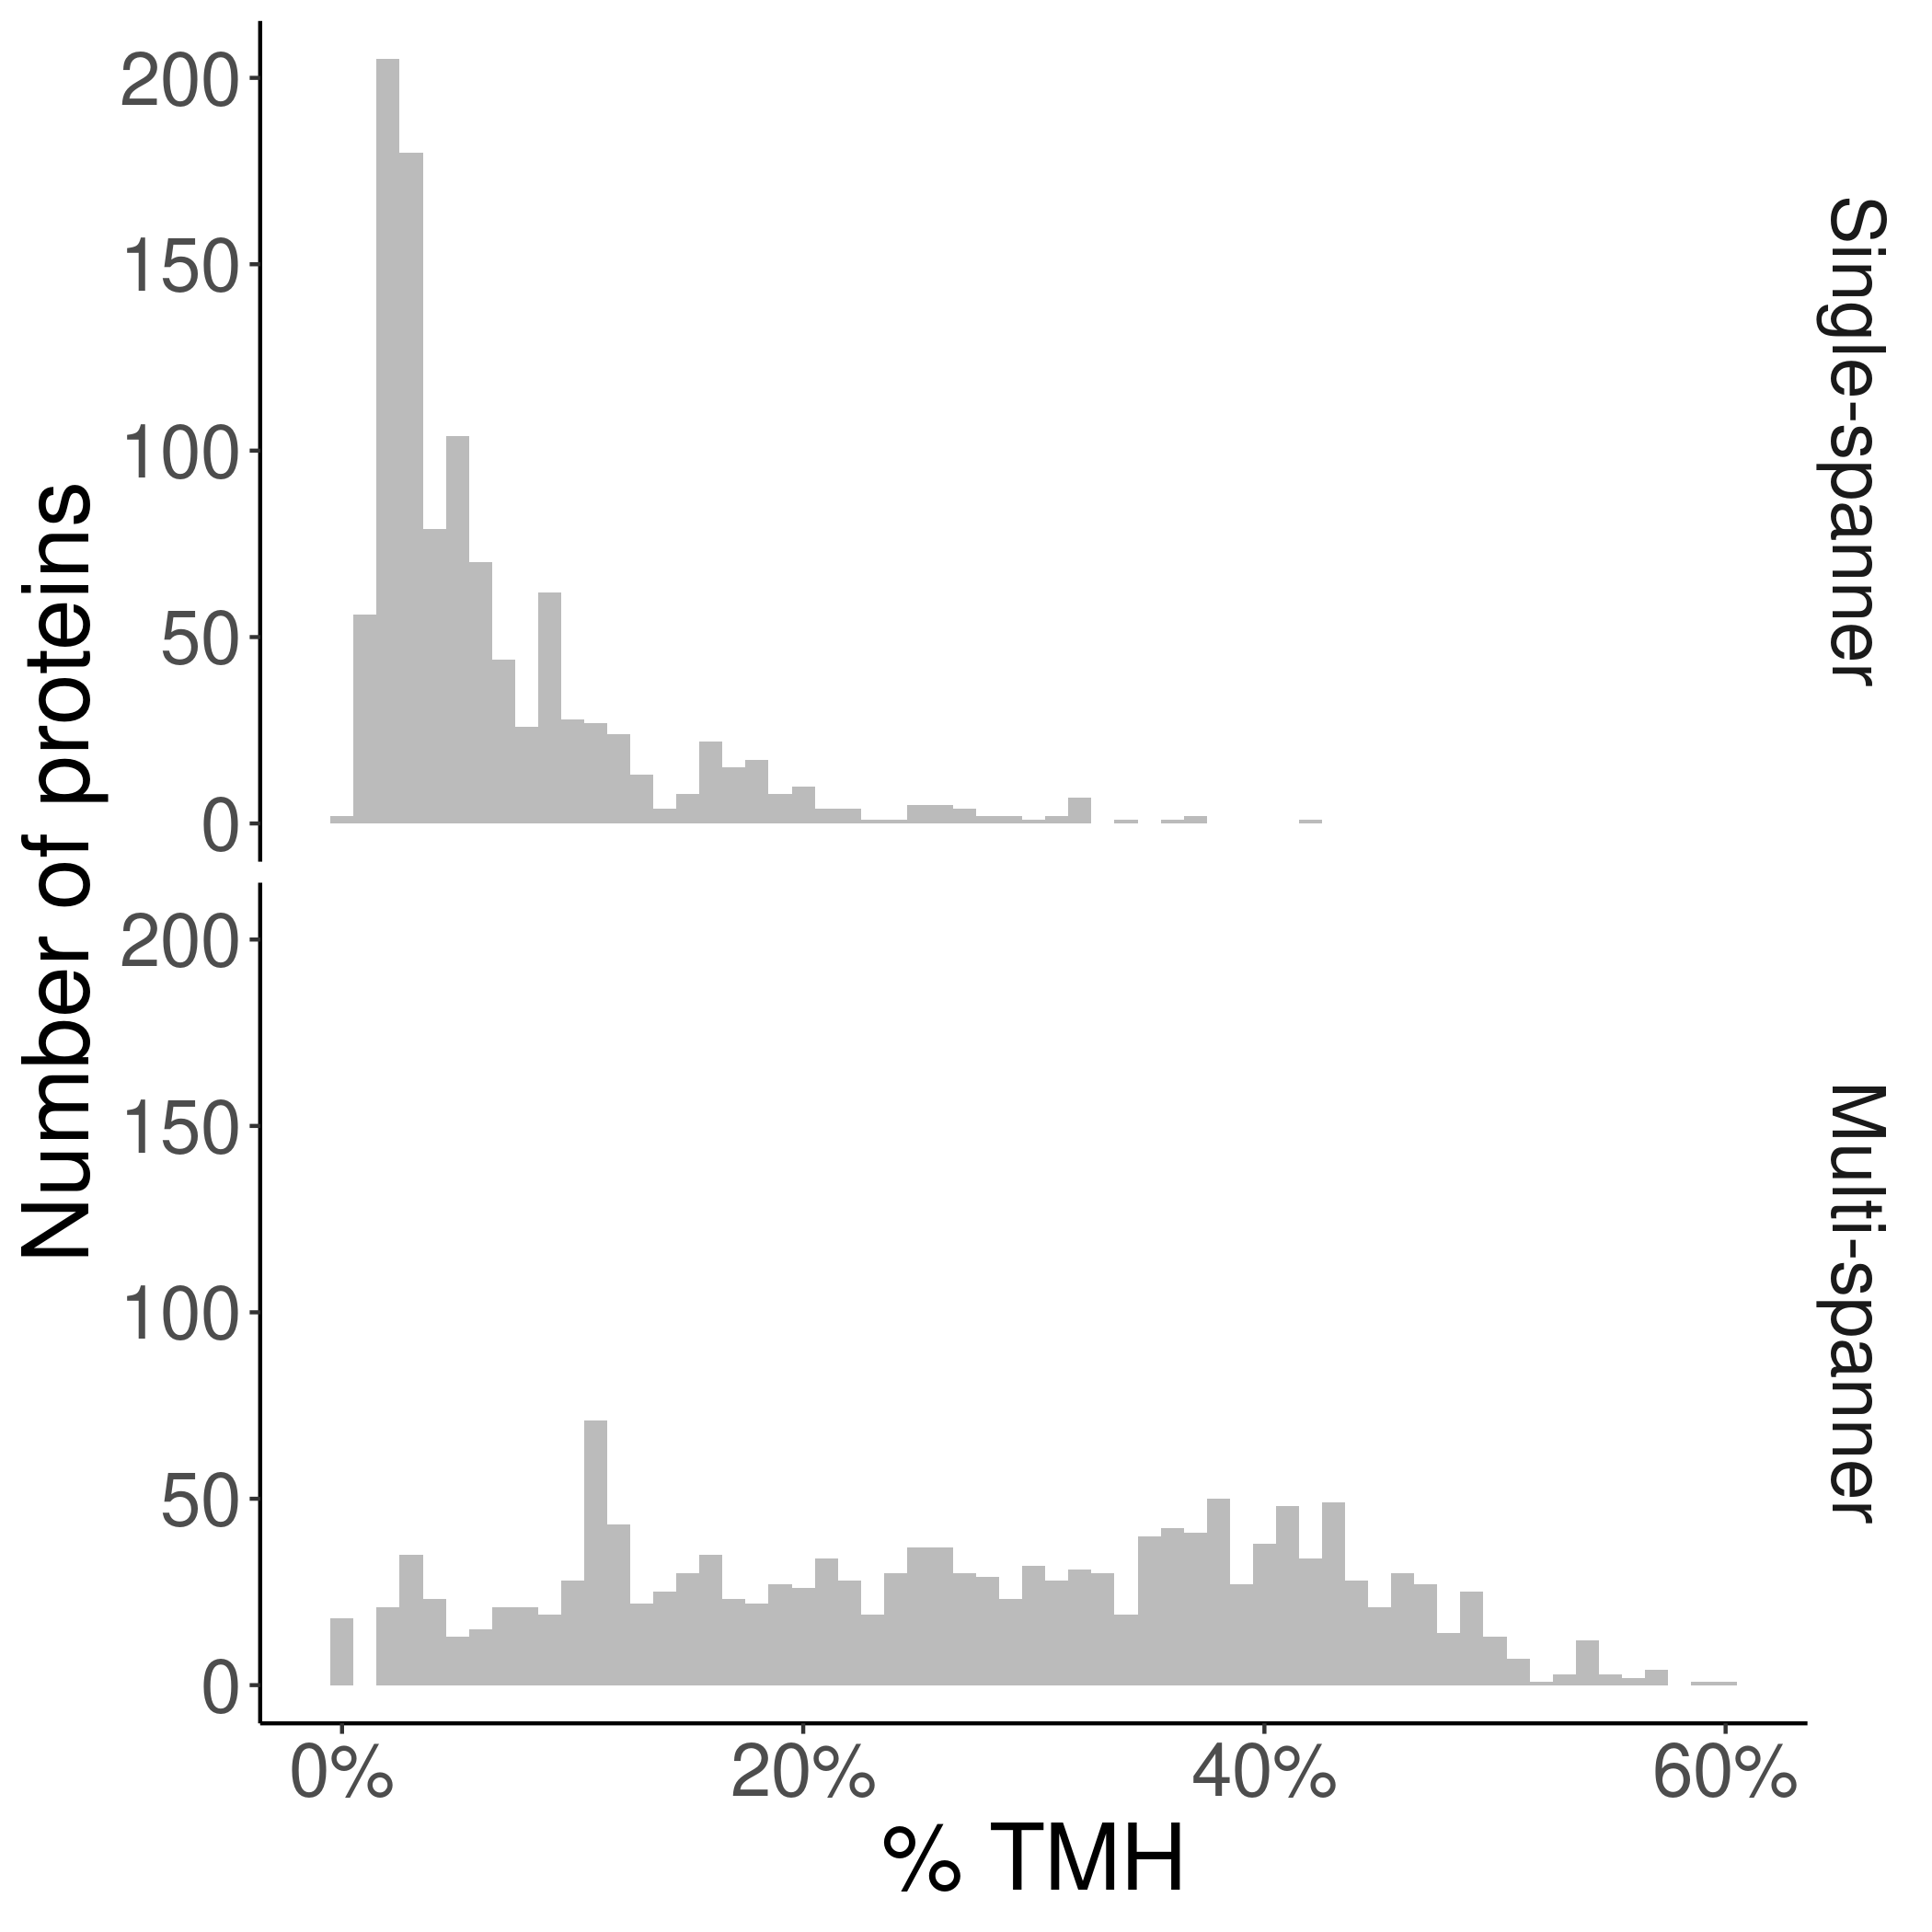
\includegraphics[width=\linewidth]{ncbi_peregrine_results/fig_f_tmh_ncbi_per_spanner.png}
    \label{fig:f_tmh_ncbi_per_spanner}
  \end{subfigure}  
  
  \caption{ \textbf{Membrane proteins with multiple TMHs are evolutionary more conserved than proteins with only a single TMH.}
      \textbf{(A)} 
      Percentage of SNPs found in TMPs predicted to have only a single
      (left) or multiple (right) TMHs.
      Each point shows for one protein the predicted percentage of amino acids that are part of a TMH ($x$-axis) and the observed occurrence of SNPs being located within a TMH ($y$-axis). The dashed diagonal lines show the line of equality (i.e., equal conservation of TMHs and soluble protein regions). 
      The diagonal red lines indicate a linear fit, the gray areas their 95\% confidence intervals.
      \textbf{(B)} 
      The number of SNPs in TMHs as expected by chance 
      and observed in the dbSNP database, 
      for TMPs with one TMH (single-spanners) and multiple TMHs (multi-spanners).
      Percentages show the relative conservation
      of SNPs in TMHs found relative to the stochastic chances.
      \textbf{(C)} 
      Distribution of the proportion of amino acids residing
      in the plasma membrane. 
     }
\end{figure}

% Process all floats before going to a next page
\clearpage

%%%%%%%%%%%%%%%%%%%%%%%%%%%%%%%%%%%%%%%%%%%%%%%%%%%%%%%%%%%%%%%%%%%%%%%%%%%%%
\newpage
\appendix
\section{Supplementary materials}

% Figures start from one and are prepended with an S
\renewcommand{\thefigure}{S\arabic{figure}}
\setcounter{figure}{0}

% Tables start from one and are prepended with an S
\renewcommand{\thetable}{S\arabic{table}}
\setcounter{table}{0}

%%%%%%%%%%%%%%%%%%%%%%%%%%%%%%%%%%%%%%%%%%%%%%%%%%%%%%%%%%%%%%%%%%%%%%%%%%%%%

%%%%%%%%%%%%%%%%%%%%%%%%%%%%%%%%%%%%%%%%%%%%%%%%%%%%%%%%%%%%%%%%%%%%%%%%%%%%%%%%
\subsection{IC50 values of binders per haplotype}
\label{subsec:ic50s_per_haplotype}
%%%%%%%%%%%%%%%%%%%%%%%%%%%%%%%%%%%%%%%%%%%%%%%%%%%%%%%%%%%%%%%%%%%%%%%%%%%%%%%%

Per target proteome (i.e. human, SARS-CoV-2, \emph{M tuberculosis}),
we collected all 9-mers (for MHC-I) and 14-mers (for MHC-II),
after removing the selenoproteins and proteins that are shorter
than the epitope length.
From these epitopes, per MHC haplotype,
we predicted the IC50 (in nM) using \verb;epitope-prediction; (for MHC-I)
and MHCnuggets (for MHC-II). 
Here, we show the IC50 value per haplotype that
is used to determine if a peptide binds to the haplotype's MHC
for MHC-I (see supplementary Table \ref{tab:ic50_binders_mhc1}) and 
MHC-II (see supplementary Table \ref{tab:ic50_binders_mhc2}).

% tab:ic50_binders_mhc1
\input{bbbq_1_smart_results/table_ic50_binders_mhc1_2.latex}

% tab:ic50_binders_mhc2
\input{bbbq_1_smart_results/table_ic50_binders_mhc2_2.latex}

% Process all floats before going to a next page
\clearpage

%%%%%%%%%%%%%%%%%%%%%%%%%%%%%%%%%%%%%%%%%%%%%%%%%%%%%%%%%%%%%%%%%%%%%%%%%%%%%%%%
\subsection{Counts}
\label{subsec:counts}
%%%%%%%%%%%%%%%%%%%%%%%%%%%%%%%%%%%%%%%%%%%%%%%%%%%%%%%%%%%%%%%%%%%%%%%%%%%%%%%%

See supplementary Tables \ref{tab:ncbi_counts_1} and \ref{tab:ncbi_counts_2}
for an overview of all amounts. 
Note that, for the analyses using the SARS-CoV-2 virus proteome,
we labeled this by its disease (\verb;covid;) to prevent typos.
In supplementary Table \ref{tab:ncbi_counts_1} there are multiple instances where
the amounts are expected to add up, yet don't, as one SNP can work on
multiple isoforms. For example, there are 9,621 unique SNPs 
found in all proteins, of which 4,219 around found in MAPs 
and 6,026 in TMPs. Apparently, 624 SNPs work on a set of isoforms that
contains both MAPs and TMPs.

% Label: tab:ncbi_counts_1
\begin{table}

\caption{\label{tab:ncbi_counts_1}Amounts. raw = all variations, including DNA variations. all\_proteins = all proteins. map = membrane associated protein. tmp = transmembrane protein. in\_tmh = in transmembrane helix of TMP. in\_sol = in soluble region of TMP. }
\centering
\begin{tabular}[t]{l|r|r|r|r|r|r}
\hline
what & raw & all\_proteins & map & tmp & in\_tmh & in\_sol\\
\hline
Number of variations & 60931 & 37831 & 16623 & 21208 & 3803 & 17405\\
\hline
Number of unique variations & 60544 & 37630 & 16606 & 21024 & 3789 & 17235\\
\hline
Number of unique SNPs & NA & 9621 & 4219 & 6026 & 1140 & 4936\\
\hline
Number of unique gene names & 953 & 911 & 457 & 605 & 325 & 590\\
\hline
Number of unique protein names & 5163 & 4780 & 2227 & 2553 & 1280 & 2467\\
\hline
Percentage TMH & NA & 10 & 0 & 19 & 26 & 18\\
\hline
\end{tabular}
\end{table}

% Label: tab:ncbi_counts_2
\begin{table}

\caption{\label{tab:ncbi_counts_2}Amounts. single\_in\_tmh = in transmembrane helix of single-spanner. single\_in\_sol = in soluble region of single-spanner. multi\_in\_tmh = in transmembrane helix of multi-spanner. multi\_in\_sol = in soluble region of multi-spanner. }
\centering
\begin{tabular}[t]{l|r|r|r|r}
\hline
what & single\_in\_tmh & single\_in\_sol & multi\_in\_tmh & multi\_in\_sol\\
\hline
Number of variations & 452 & 7734 & 3351 & 9671\\
\hline
Number of unique variations & 451 & 7733 & 3338 & 9502\\
\hline
Number of unique SNPs & 160 & 2393 & 994 & 2762\\
\hline
Number of unique gene names & 96 & 282 & 243 & 344\\
\hline
Number of unique protein names & 304 & 1032 & 976 & 1435\\
\hline
Percentage TMH & 11 & 5 & 35 & 26\\
\hline
\end{tabular}
\end{table}

% Process all floats before going to a next page
\clearpage

%%%%%%%%%%%%%%%%%%%%%%%%%%%%%%%%%%%%%%%%%%%%%%%%%%%%%%%%%%%%%%%%%%%%%%%%%%%%%%%%
\subsection{Relative positions}
%%%%%%%%%%%%%%%%%%%%%%%%%%%%%%%%%%%%%%%%%%%%%%%%%%%%%%%%%%%%%%%%%%%%%%%%%%%%%%%%

See Supplementary Figure \ref{fig:snp_rel_pos}
for the distribution of the relative position of the SNPs.

\begin{figure}[!htbp]
  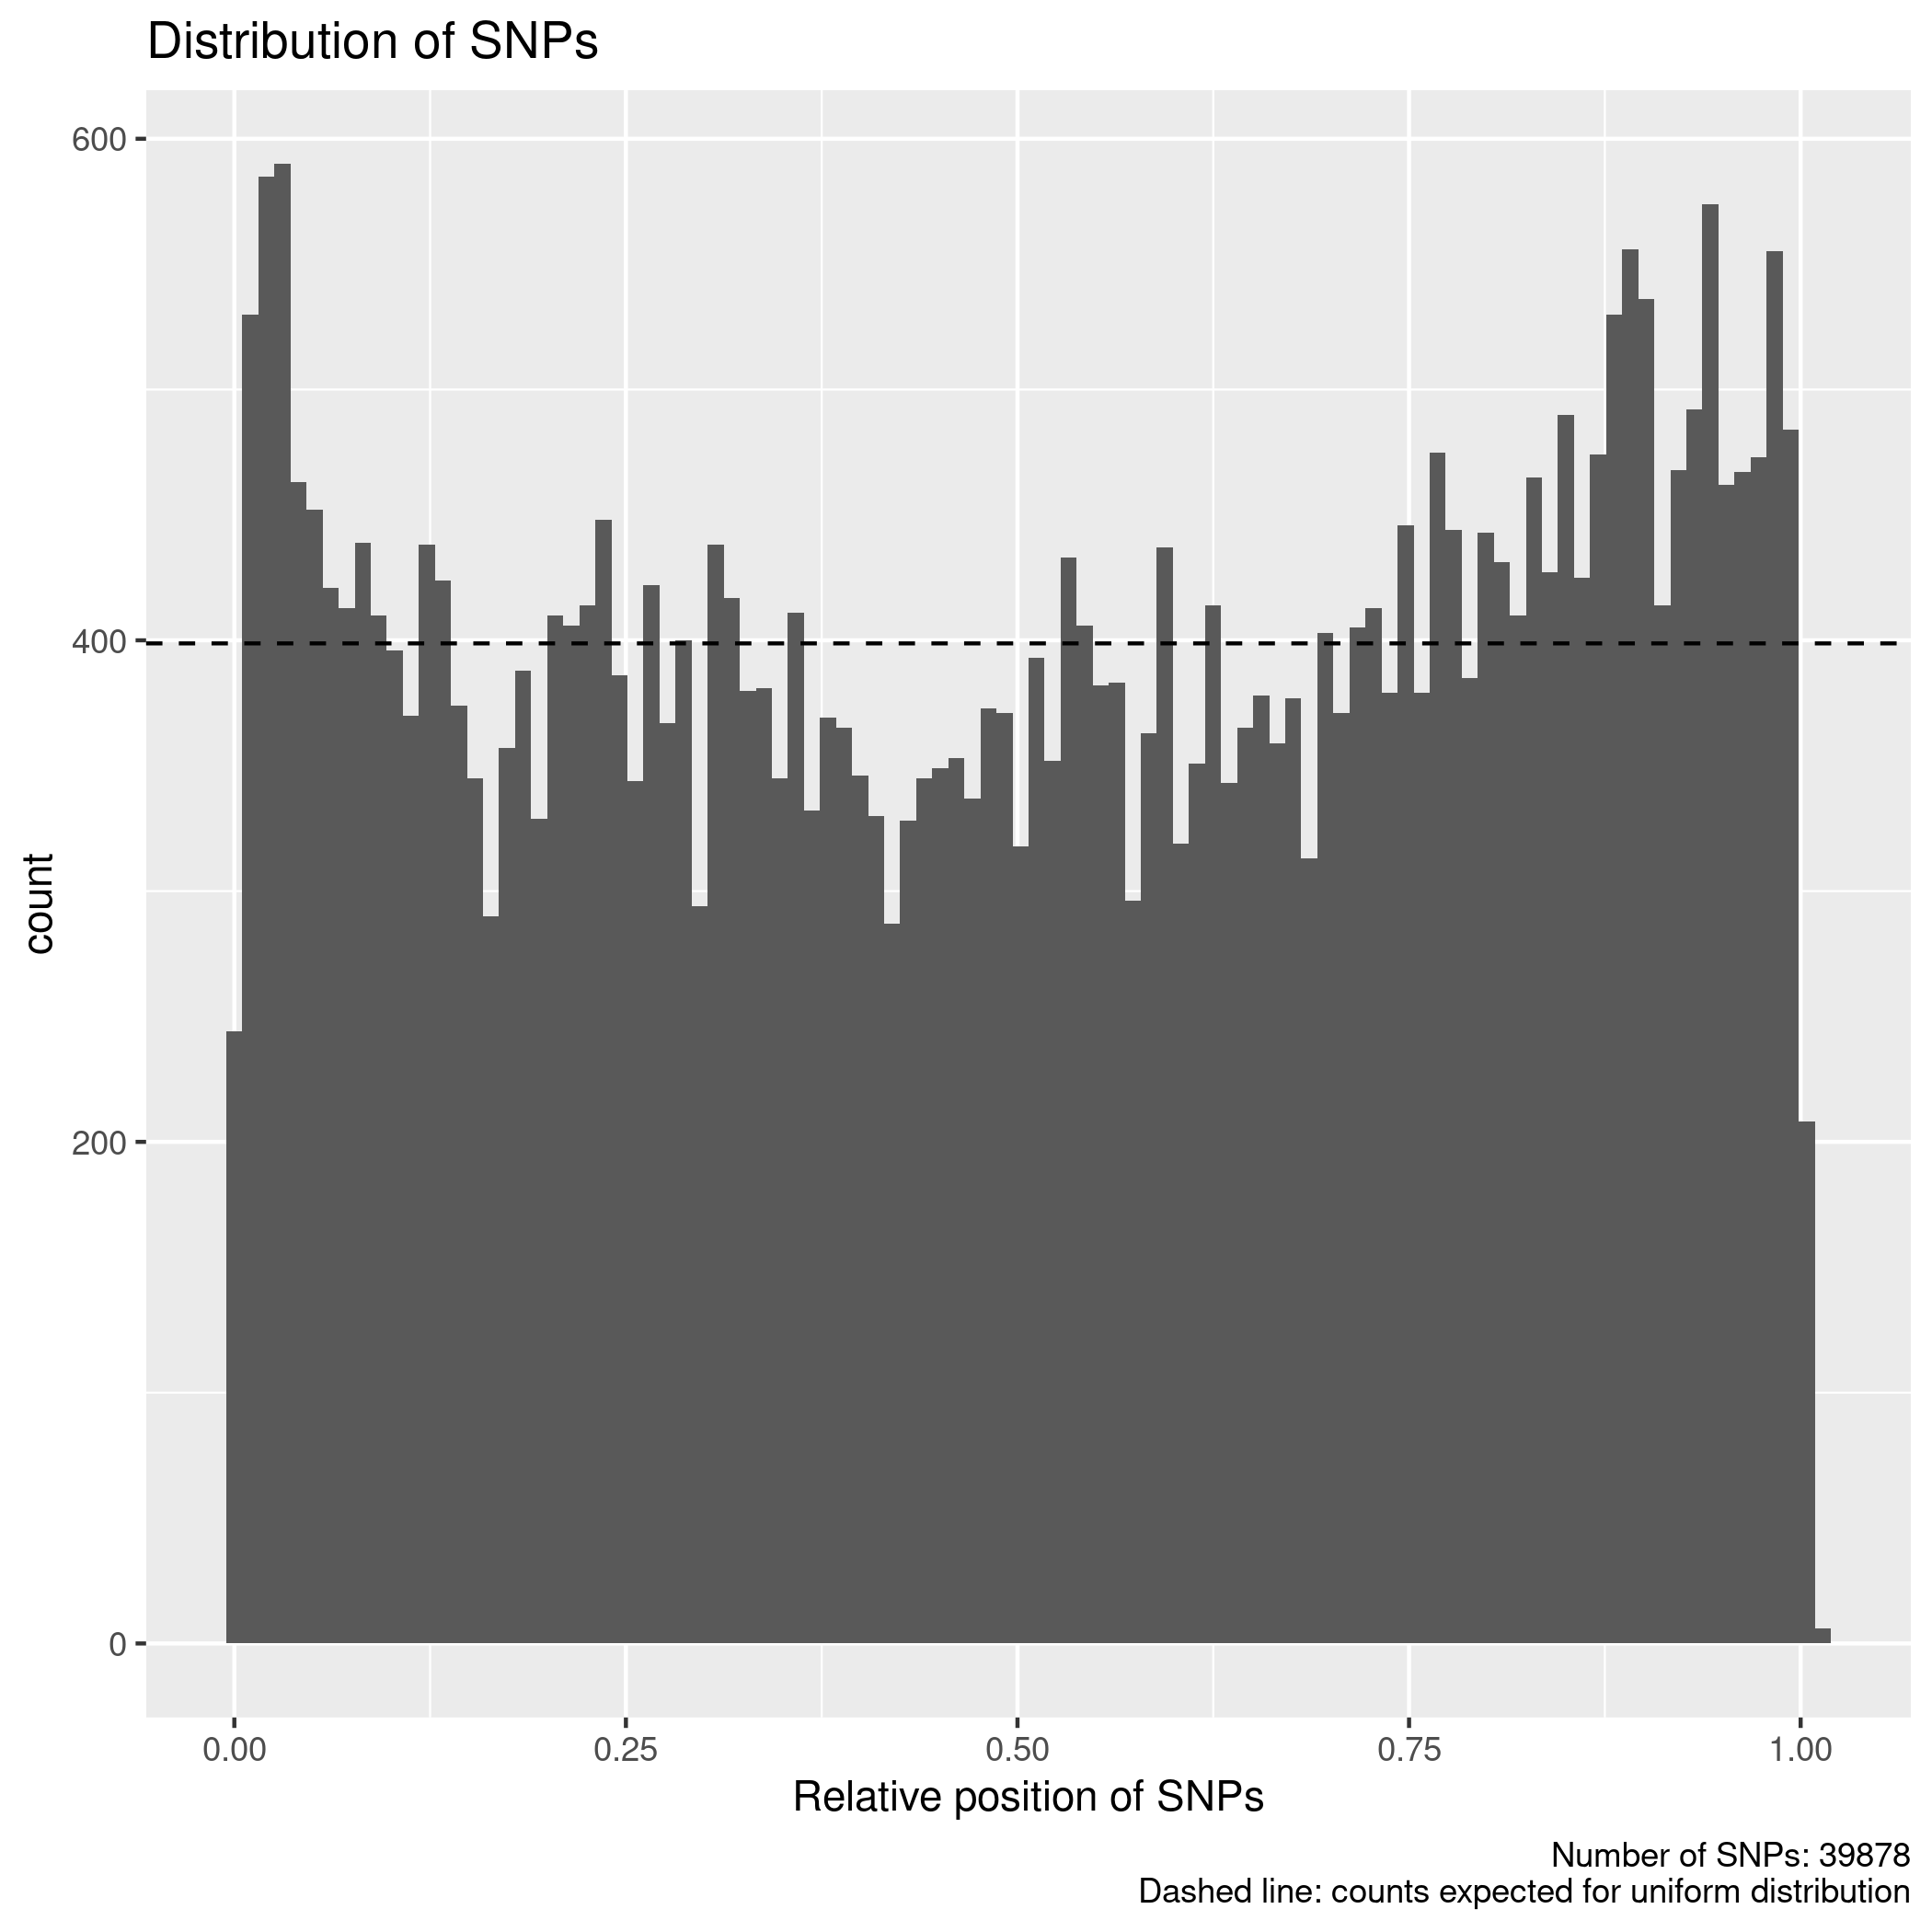
\includegraphics[width=\textwidth]{ncbi_peregrine_results/fig_snp_rel_pos.png}
  \caption{
    Distribution of the relative position of the SNPs used,
    where a relative position of zero denotes the first amino
    acid at the N-terminus, where a relative position of one
    indicates the last residue at the C-terminus.
  }
  \label{fig:snp_rel_pos}
\end{figure}

% Process all floats before going to a next page
\clearpage

%%%%%%%%%%%%%%%%%%%%%%%%%%%%%%%%%%%%%%%%%%%%%%%%%%%%%%%%%%%%%%%%%%%%%%%%%%%%%%%%
\subsection{Presentation of TMH-derived epitopes}
%%%%%%%%%%%%%%%%%%%%%%%%%%%%%%%%%%%%%%%%%%%%%%%%%%%%%%%%%%%%%%%%%%%%%%%%%%%%%%%%

See supplementary Table \ref{tab:tmh_binders_mhc2} 
for the percentage of MHC-II 14-mers overlapping with TMH.

% Label: tab:tmh_binders_mhc2
\input{bbbq_1_smart_results/table_tmh_binders_mhc2_2.latex}

% Process all floats before going to a next page
\clearpage

%%%%%%%%%%%%%%%%%%%%%%%%%%%%%%%%%%%%%%%%%%%%%%%%%%%%%%%%%%%%%%%%%%%%%%%%%%%%
\subsection{The percentage of TMH-derived epitopes from IEDB epitopes}
%%%%%%%%%%%%%%%%%%%%%%%%%%%%%%%%%%%%%%%%%%%%%%%%%%%%%%%%%%%%%%%%%%%%%%%%%%%%

We display the over-presentation of epitopes taken from the
IEDB database, for two assays: an MHC ligand assay (Figure \ref{fig:2a})
and a T cell assay (see figure \ref{fig:t_cells_present_tmh_derived_epitopes}),
as a bar plot.
Supplementary Table \ref{tab:elution} below shows the
exact numbers. \textbf{GEERT: spelfout in legenda: brackets ipv braces}

% tab:elution
% latex table generated in R 4.1.1 by xtable 1.8-4 package
% Fri Oct 29 12:40:25 2021
\begin{table}[ht]
\centering
\begin{tabular}{llll}
  \hline
MHC class & Tool & Dataset & n \\ 
  \hline
I & PureseqTM & schellens & 1.38\% (109/7897) \\ 
  I & PureseqTM & iedb & 6.81\% (43/631) \\ 
  I & TMHMM & schellens & 1.43\% (113/7897) \\ 
  I & TMHMM & iedb & 7.13\% (45/631) \\ 
  II & PureseqTM & bergseng & 3.92\% (498/12712) \\ 
  II & PureseqTM & iedb & 0.29\% (4/1364) \\ 
  II & TMHMM & bergseng & 3.96\% (504/12712) \\ 
  II & TMHMM & iedb & 1.39\% (19/1364) \\ 
   \hline
\end{tabular}
\caption{Percentage of epitopes derived from a TMH found in the two elution studies, for the two different kind of topology prediction tools. The values between braces show the the number of epitopes that were predicted to overlapping with a TMH per all epitopes that could be uniquely mapped to the representative human reference proteome.} 
\label{tab:elution}
\end{table}


% Process all floats before going to a next page
\clearpage

%%%%%%%%%%%%%%%%%%%%%%%%%%%%%%%%%%%%%%%%%%%%%%%%%%%%%%%%%%%%%%%%%%%%%%%%%%%%%%%%
\subsection{Correlation of epitope presentation}
%%%%%%%%%%%%%%%%%%%%%%%%%%%%%%%%%%%%%%%%%%%%%%%%%%%%%%%%%%%%%%%%%%%%%%%%%%%%%%%%

In the main text of this research, we use two sources of epitopes
to determine if TMH-derived epitopes are presented.
The first source of epitopes are all the 9-mers (for MHC-I) (and 14-mers for MHC-II)
derived from a human reference proteome, where this over-presentation
is displayed in figure \ref{fig:bbbq_1_smart_results}.
The second source of epitopes are those that are present in the IEDB
that are obtained from MHC ligand assays,
as displayed in figure \ref{fig:2a}.

Here we correlate between the over-presentation of TMH-derived
epitopes between these two sources of data.
Figure \ref{fig:thm_presentation_correlation} shows per haplotype
the percentage of TMH-derived epitopes, with a linear trendline.

\begin{figure}[!htbp]
  \centering
  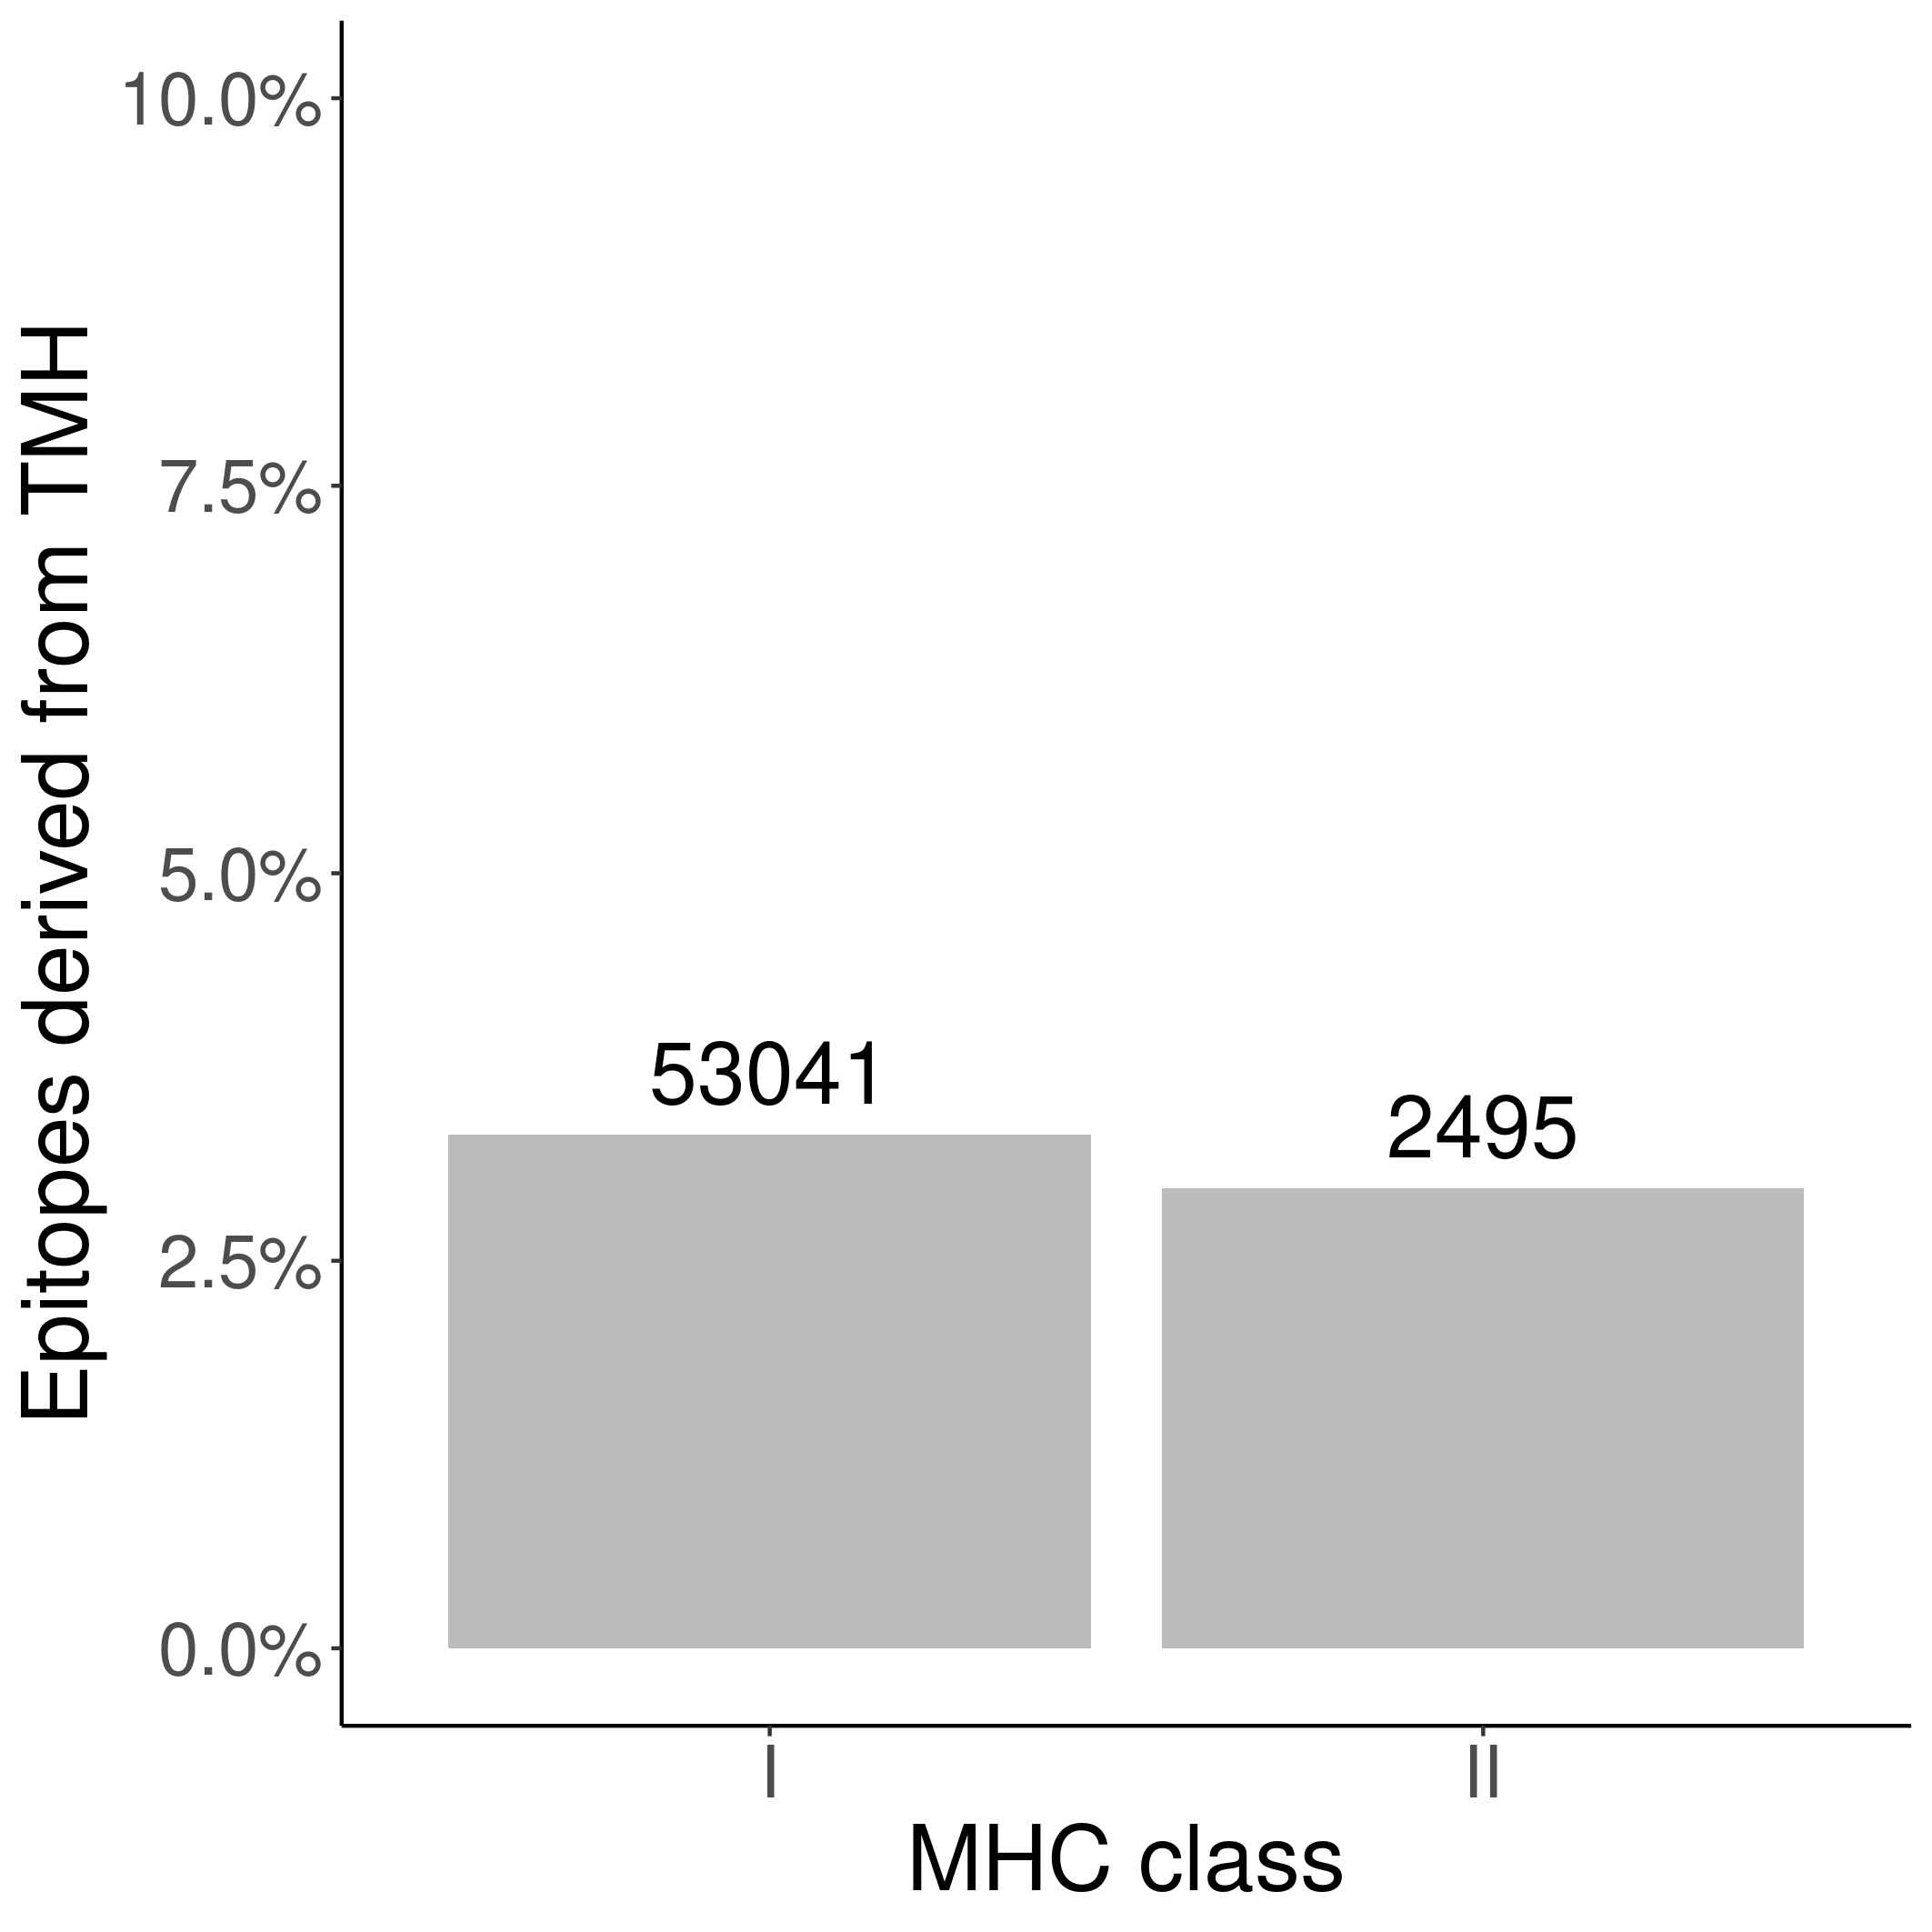
\includegraphics[width=0.5\textwidth]{bbbq_article_issue_157/figure_2c.png}
  \caption{
    \textbf{
      TMH-derived epitopes are over-presented when using
      predicted as well as experimental data
    }
    For the MHC class I alleles, the over-presentation of
    TMH-derived epitopes is correlated between 
    IEDB MHC ligand epitopes (horizontal axis) and the 9-mers
    derived from a human reference proteome (vertical axis).
    Alleles are listed in Table \ref{tab:haplotype_abbreviations}).
    The trendline shows the linear correlation between these
    percentages, where the gray area is the 95\% confidence interval.
  }
  \label{fig:thm_presentation_correlation}
\end{figure}

% Process all floats before going to a next page
\clearpage

%%%%%%%%%%%%%%%%%%%%%%%%%%%%%%%%%%%%%%%%%%%%%%%%%%%%%%%%%%%%%%%%%%%%%%%%%%%%%%%%
\subsection{Presentation of TMH-derived epitopes \emph{in vivo} in T cells}
%%%%%%%%%%%%%%%%%%%%%%%%%%%%%%%%%%%%%%%%%%%%%%%%%%%%%%%%%%%%%%%%%%%%%%%%%%%%%%%%

Figure \ref{fig:t_cells_present_tmh_derived_epitopes} 
shows the percentage of TMH-derived
epitopes of the reported epitopes that for which T-cell responses were established. 
The data was obtained from the IEDB and includes only the MHC
alleles used in this study. As there are many (especially class II)
MHC alleles, only a small percentage of the full IEDB data could be used.


\begin{figure}[!htbp]
  \centering
  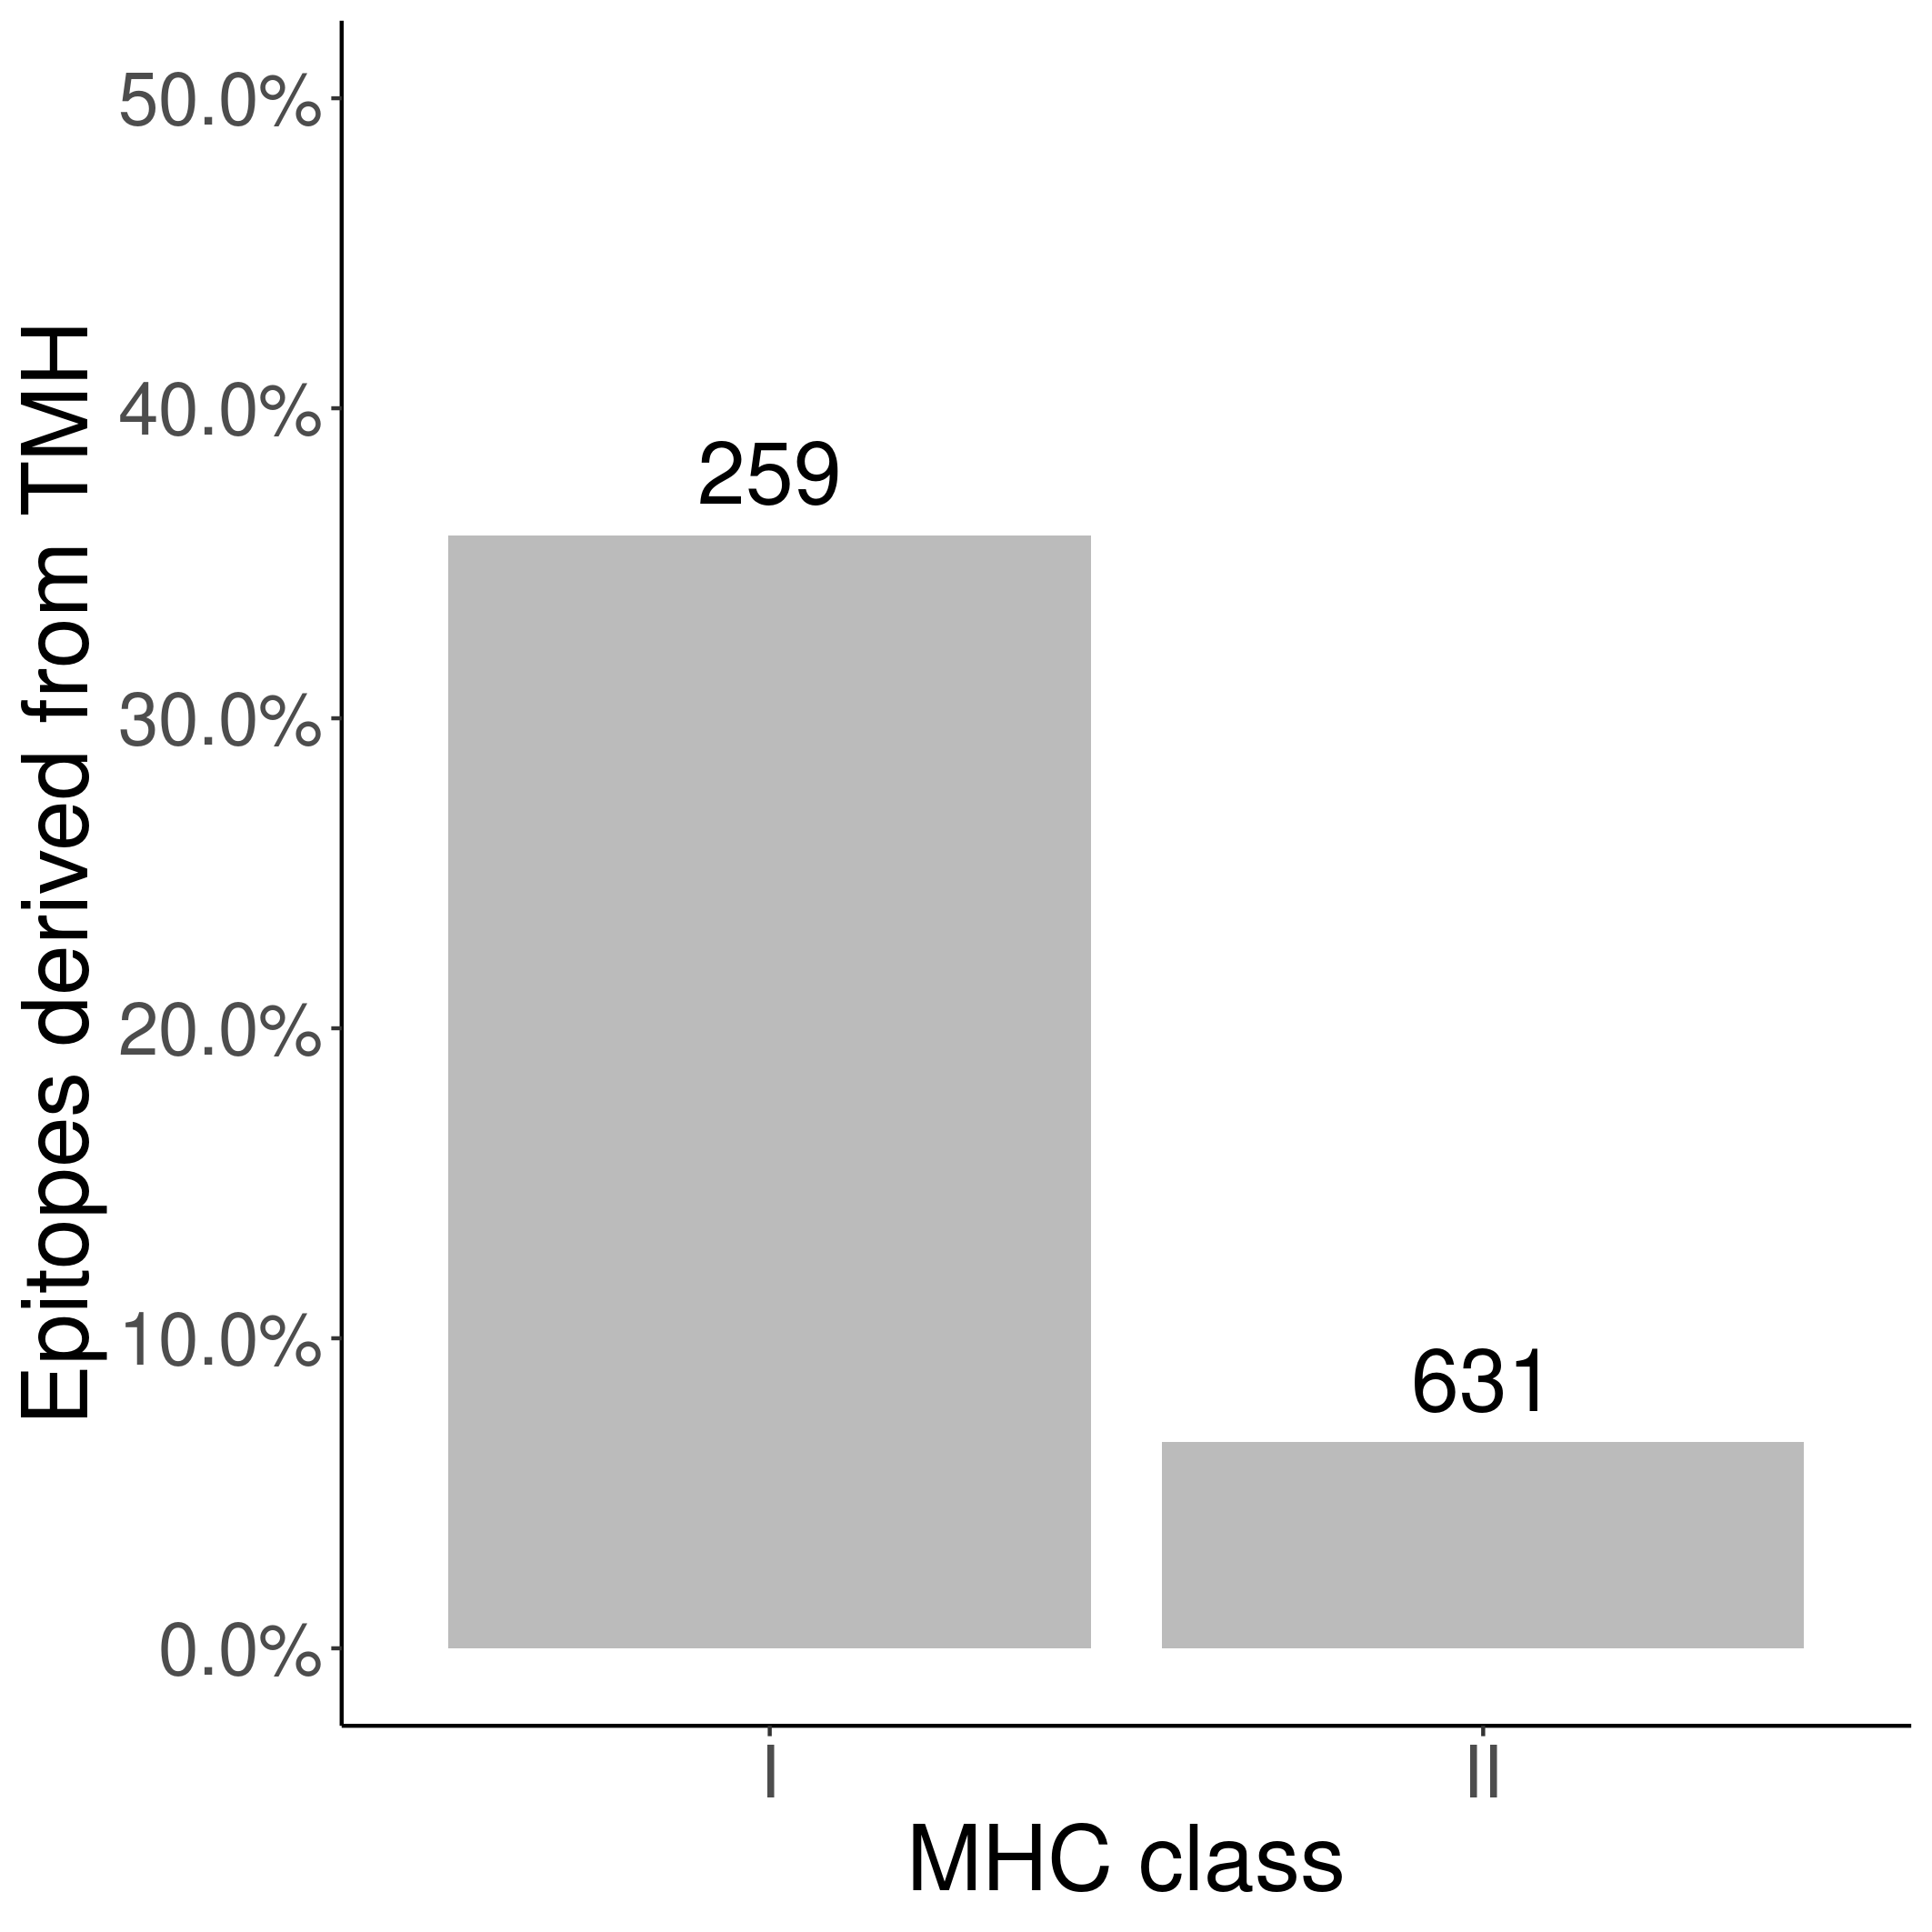
\includegraphics[width=0.5\textwidth]{bbbq_article_issue_157/figure_2d.png}
  \caption{
    \textbf{
      TMH-derived epitopes evoke T-cell responses 
      }
    The numbers above the bars denotes the number of epitopes
    found in the IEDB for the MHC alleles used in this study.
  }
  \label{fig:t_cells_present_tmh_derived_epitopes}
\end{figure}

% Process all floats before going to a next page
\clearpage

%%%%%%%%%%%%%%%%%%%%%%%%%%%%%%%%%%%%%%%%%%%%%%%%%%%%%%%%%%%%%%%%%%%%%%%%%%%%%%%%
\subsection{Presentation of TMH-derived epitopes}
%%%%%%%%%%%%%%%%%%%%%%%%%%%%%%%%%%%%%%%%%%%%%%%%%%%%%%%%%%%%%%%%%%%%%%%%%%%%%%%%

See supplementary Table \ref{tab:tmh_binders_mhc1} 
for the percentage of MHC-I 9-mers overlapping with TMH.

% Label: tab:tmh_binders_mhc1
\input{bbbq_1_smart_results/table_tmh_binders_mhc1_2.latex}

Supplementary Table \ref{tab:haplotype_abbreviations} shows the
shorthand notation for the HLA haplotypes.

% Label: tab:haplotype_abbreviations
% latex table generated in R 4.0.4 by xtable 1.8-4 package
% Mon Apr  5 12:14:41 2021
\begin{table}[ht]
\centering
\begin{tabular}{rl}
  \hline
index & haplotype\_name \\ 
  \hline
  1 & HLA-A*01:01 \\ 
    2 & HLA-A*02:01 \\ 
    3 & HLA-A*03:01 \\ 
    4 & HLA-A*24:02 \\ 
    5 & HLA-A*26:01 \\ 
    6 & HLA-B*07:02 \\ 
    7 & HLA-B*08:01 \\ 
    8 & HLA-B*18:01 \\ 
    9 & HLA-B*27:05 \\ 
   10 & HLA-B*39:01 \\ 
   11 & HLA-B*40:02 \\ 
   12 & HLA-B*58:01 \\ 
   13 & HLA-B*15:01 \\ 
    1 & HLA-DRB1*0101 \\ 
    2 & HLA-DRB1*0301 \\ 
    3 & HLA-DRB1*0401 \\ 
    4 & HLA-DRB1*0405 \\ 
    5 & HLA-DRB1*0701 \\ 
    6 & HLA-DRB1*0802 \\ 
    7 & HLA-DRB1*0901 \\ 
    8 & HLA-DRB1*1101 \\ 
    9 & HLA-DRB1*1201 \\ 
   10 & HLA-DRB1*1302 \\ 
   11 & HLA-DRB1*1501 \\ 
   12 & HLA-DRB3*0101 \\ 
   13 & HLA-DRB3*0202 \\ 
   14 & HLA-DRB4*0101 \\ 
   15 & HLA-DRB5*0101 \\ 
   16 & HLA-DQA1*0501/DQB1*0201 \\ 
   17 & HLA-DQA1*0501/DQB1*0301 \\ 
   18 & HLA-DQA1*0301/DQB1*0302 \\ 
   19 & HLA-DQA1*0401/DQB1*0402 \\ 
   20 & HLA-DQA1*0101/DQB1*0501 \\ 
   21 & HLA-DQA1*0102/DQB1*0602 \\ 
   \hline
\end{tabular}
\caption{Abbreviations of the haplotype names} 
\label{tab:haplotype_abbreviations}
\end{table}


Supplementary Tables \ref{tab:tmh_binders_mhc1} and \ref{tab:tmh_binders_mhc2}
show the exact number of binders, binders that overlap with TMHs
and the percentage of binders that overlap with TMHs, as
visualized by figure \ref{fig:bbbq_1_smart_results}.

% Process all floats before going to a next page
\clearpage

%%%%%%%%%%%%%%%%%%%%%%%%%%%%%%%%%%%%%%%%%%%%%%%%%%%%%%%%%%%%%%%%%%%%%%%%%%%%%
\subsection{Differences with Bianchi et al., 2017}
%%%%%%%%%%%%%%%%%%%%%%%%%%%%%%%%%%%%%%%%%%%%%%%%%%%%%%%%%%%%%%%%%%%%%%%%%%%%%

A part of this study does the same analysis as Bianchi et al., 2017.
mainly concern the use of different
software and a different definition of what an MHC binder is.

% \paragraph{Definition of what a binder is}

The earlier study defined a peptide an MHC binder 
if \emph{within the protein} in which it was found, 
is was among the peptides with the 2\% lowest IC50 values.
This can be seen at \url{https://github.com/richelbilderbeek/bianchi_et_al_2017/blob/master/predict-binders.R},
where the binders are written to file.

However, in this study, an MHC binder is defined as a peptide within a \emph{proteome} in which it is found, that is among the peptides with the 2\% lowest IC50 values.
Subsection \ref{subsec:ic50s_per_haplotype} shows the IC50 values
for a binder per haplotype. 

% \paragraph{Selenoproteins}

Our previous study used the TMHMM web server
to predict TMHs.
The desktop version of TMHMM, however, gives an
error message on the 25 selenoproteins found in the human
reference proteome.
For the sake of reproducible research, we used the desktop version (as
we can call it from scripts) and, due to this, we removed the
selenoproteins from this analysis.

% \paragraph{Compare results in figure}

To verify if the previous and the current method give rise to
notable difference, we show a side-by-side comparison
in figures \ref{fig:bianch_et_al_2017_1a} and \ref{fig:bilderbeek_et_al_2021_1a}.
The figures that haplotypes that over-present or under-present TMH-derived epitopes,
do so in both studies. The extent to which TMH-derived epitopes are
presented, however, is more extreme in our current setup.

\begin{figure}
  \centering
  \begin{subfigure}[t]{0.45\textwidth}
    \centering
    \caption{}
    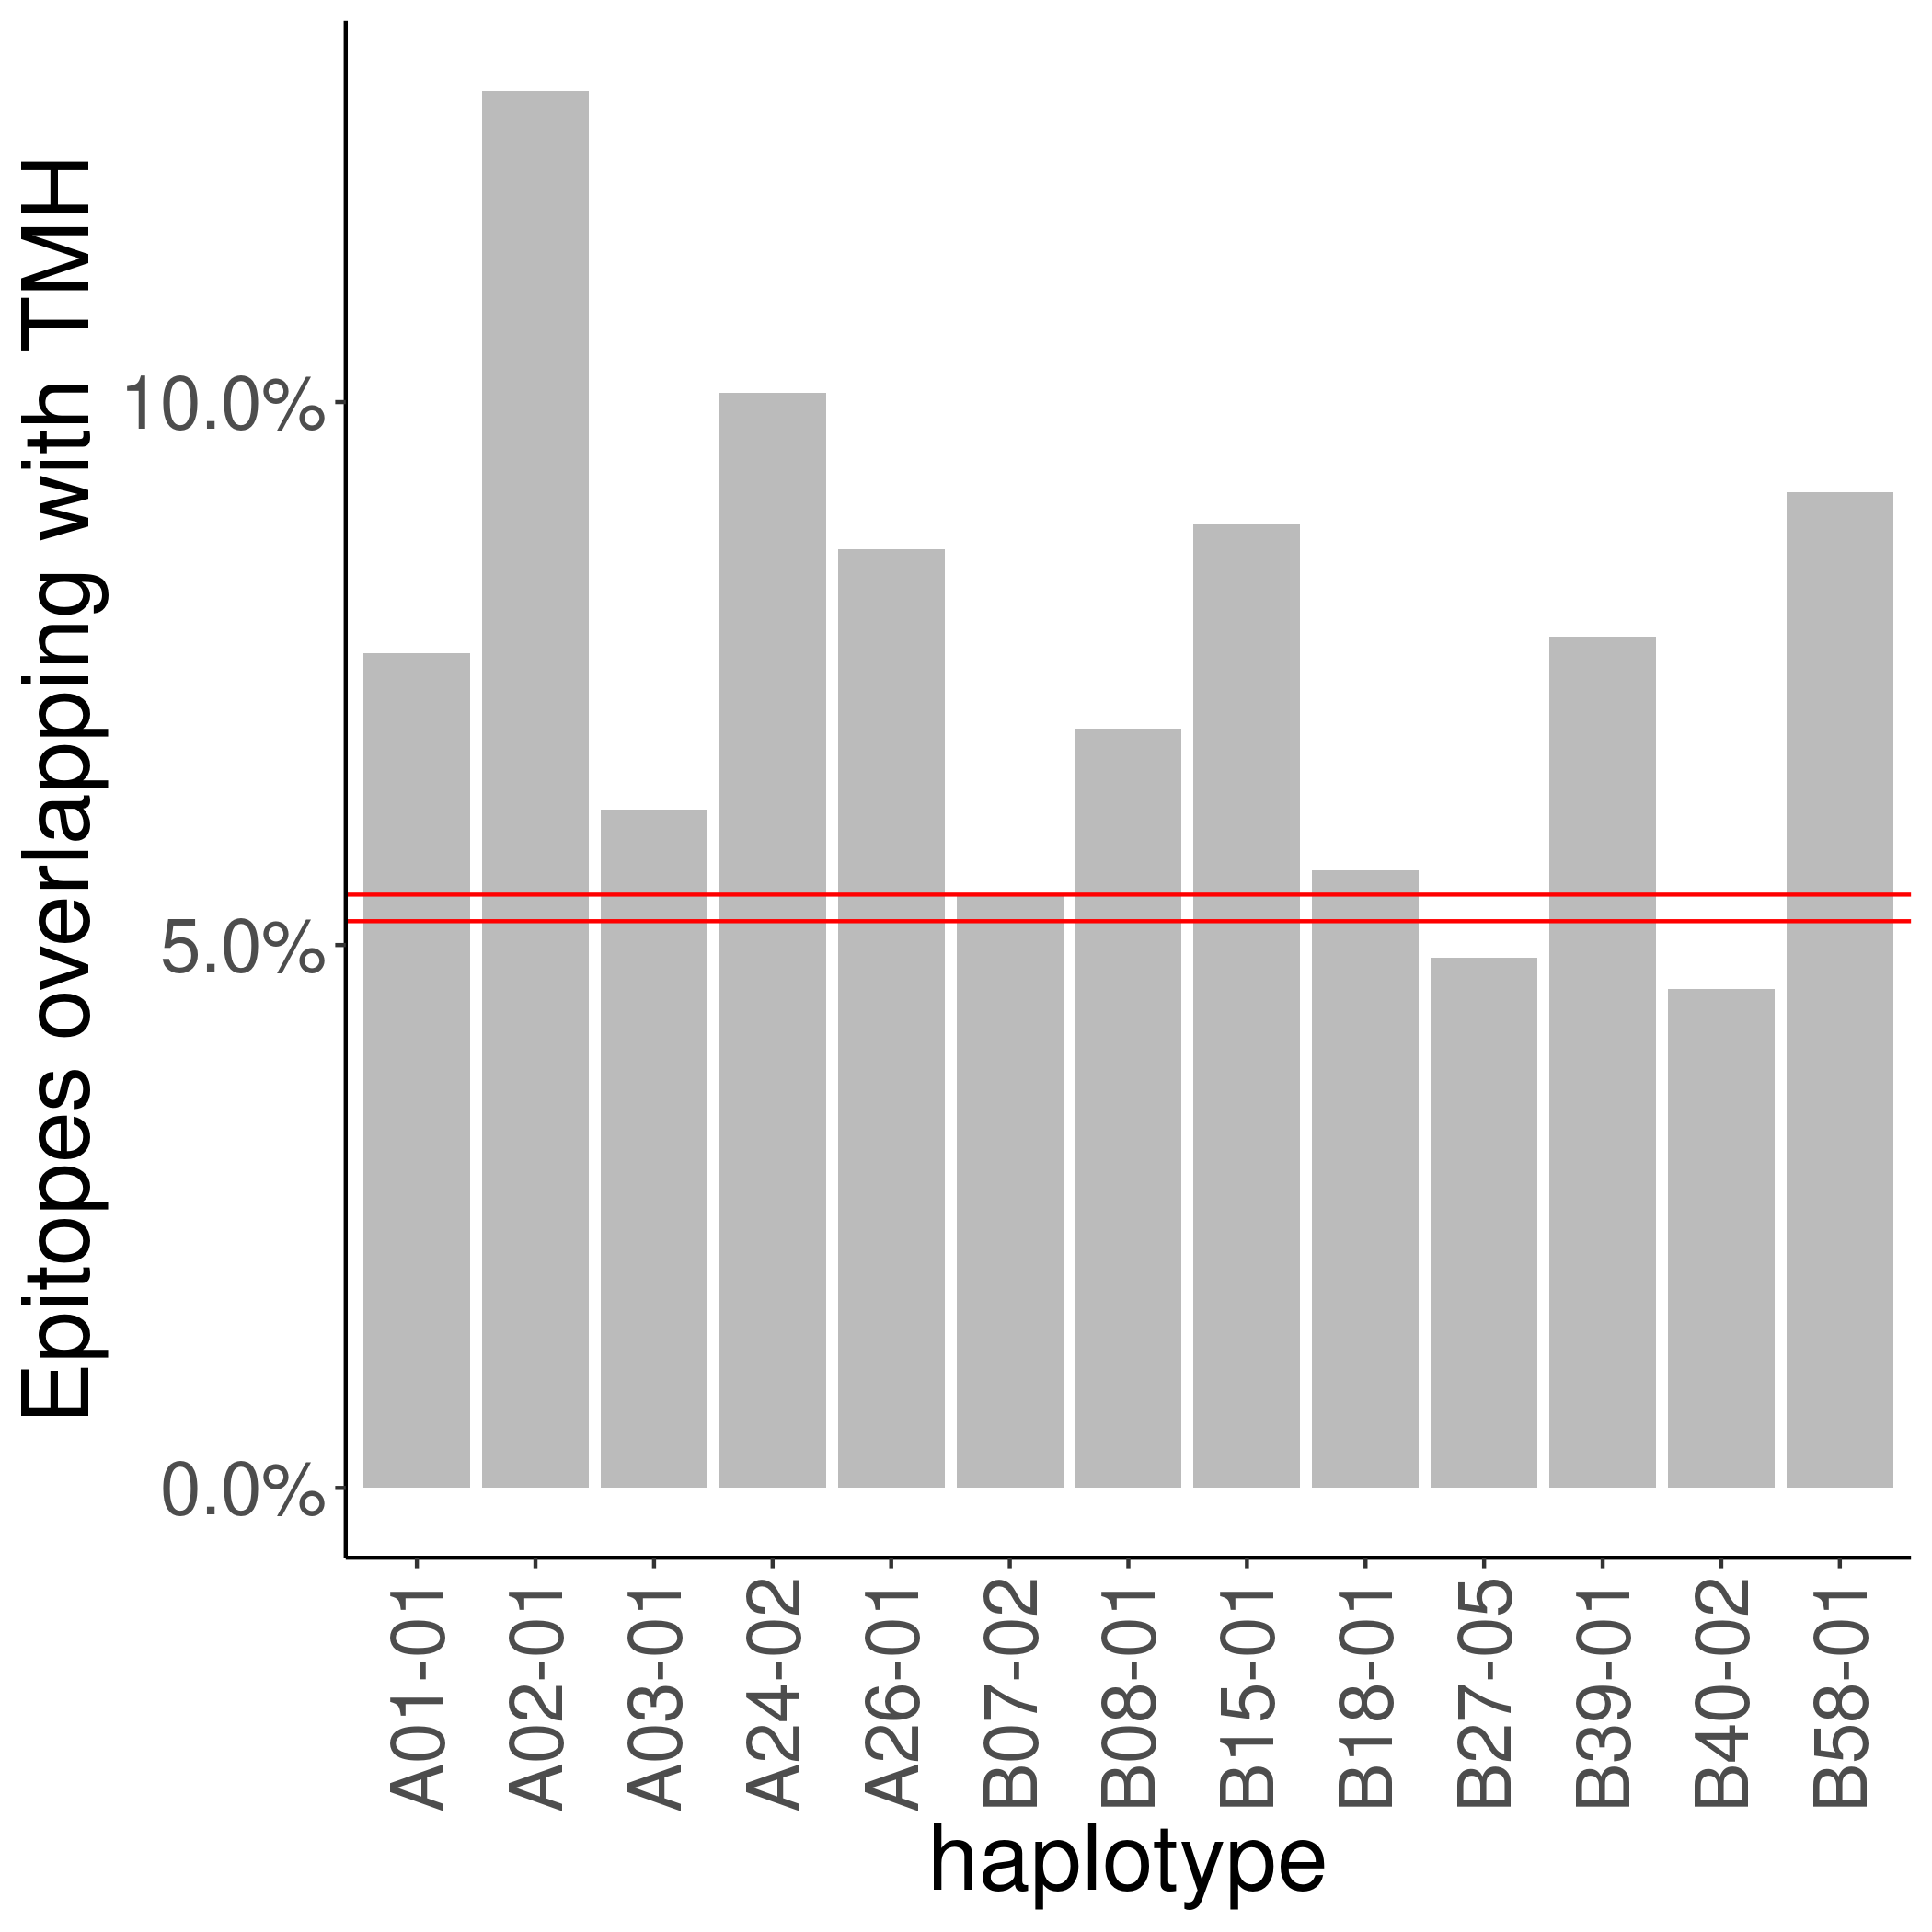
\includegraphics[width=\linewidth]{bianchi_et_al_2017_results/figure-1-a.png} % use same naming as them
    \label{fig:bianch_et_al_2017_1a}
  \end{subfigure}
  \hfill
  \begin{subfigure}[t]{0.45\textwidth}
    \centering
    \caption{}
    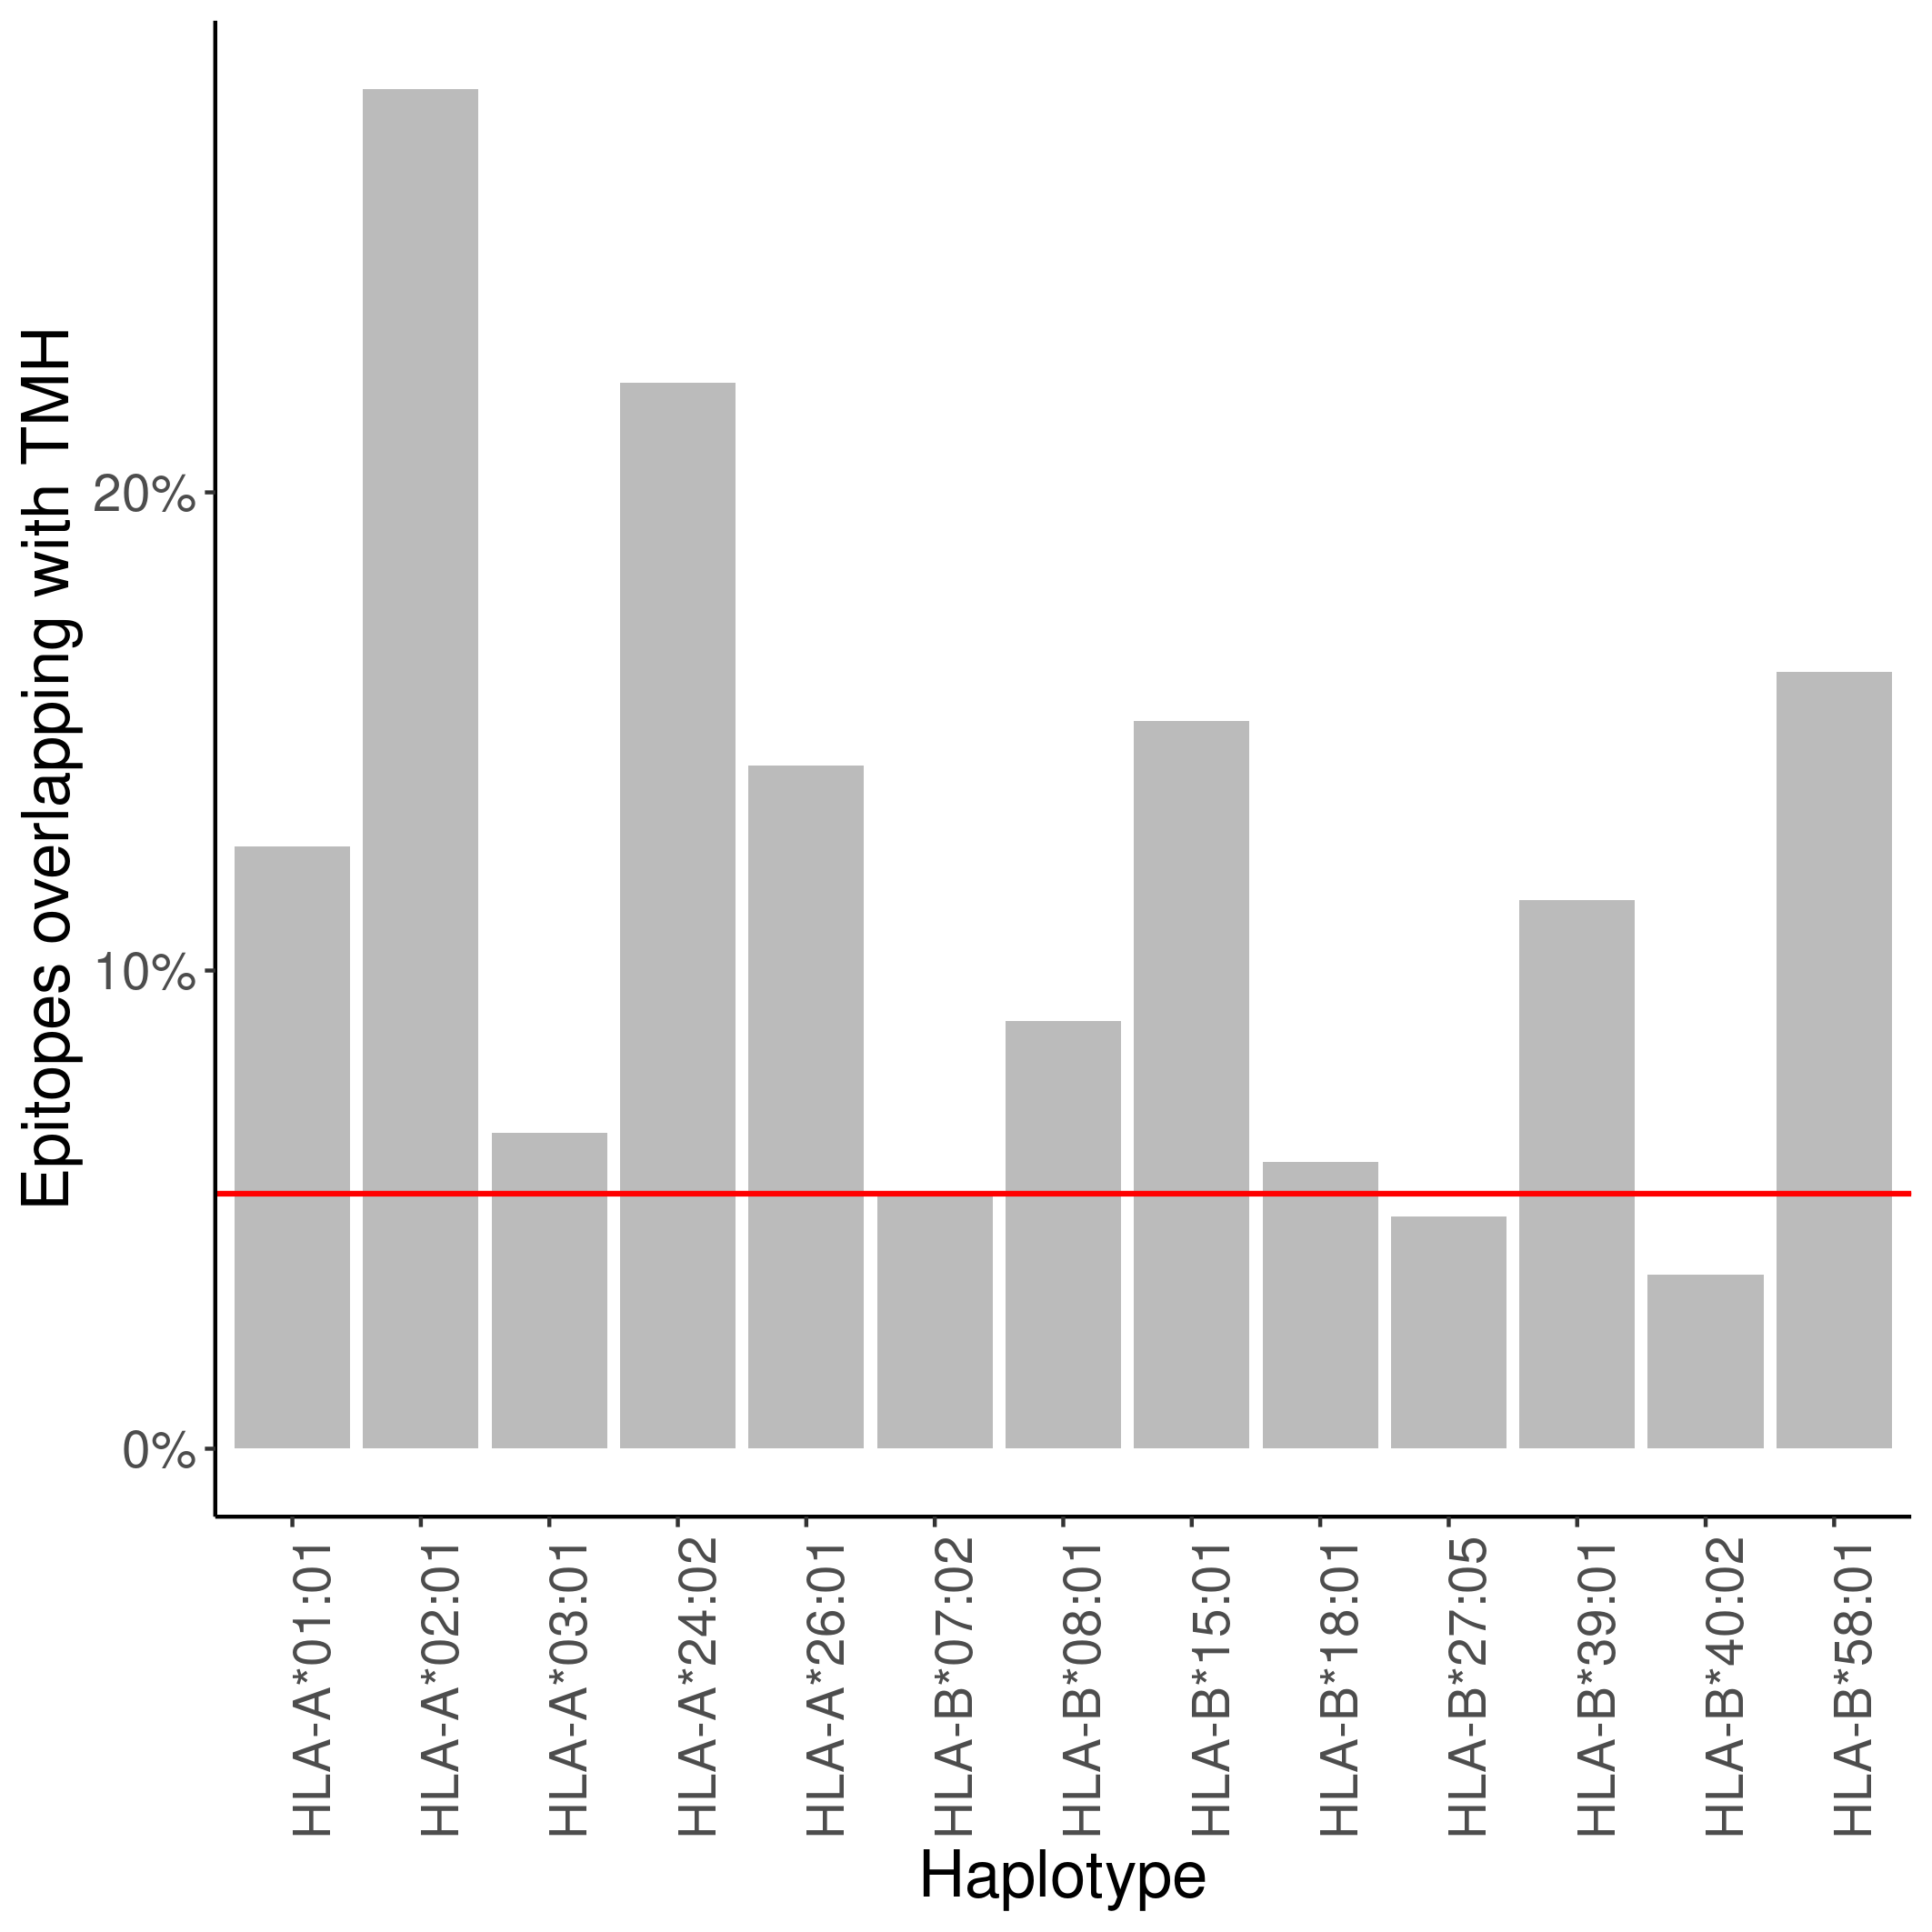
\includegraphics[width=\linewidth]{bbbq_1_smart_results/fig_f_tmh_2_human_mhc1.png}
    \label{fig:bilderbeek_et_al_2021_1a}
  \end{subfigure}

  \caption{
    \textbf{(A)} 
    Results for \cite{bianchi2017}. 
    Dashed lines denotes the coincidence interval.
    \textbf{(B)}
    Results for this study.
    Dashed line denotes the percentage as expected by chance.
  }
\end{figure}

% Process all floats before going to a next page
\clearpage

%%%%%%%%%%%%%%%%%%%%%%%%%%%%%%%%%%%%%%%%%%%%%%%%%%%%%%%%%%%%%%%%%%%%%%%%%%%%%%%%
\subsection{Prediction software used}
\label{subsec:prediction_software_used}
%%%%%%%%%%%%%%%%%%%%%%%%%%%%%%%%%%%%%%%%%%%%%%%%%%%%%%%%%%%%%%%%%%%%%%%%%%%%%%%%

\begin{table}[]
  \begin{tabular}{llll}
    Goal & Tool & Reference \\ 
    \hline
    Predict topology                  & TMHMM                     & \cite{krogh2001predicting} \\
    Predict topology                  & PureseqTM                 & \cite{wang2019efficient} \\
    Predict epitopes MHC-I            & \verb;epitope-prediction; & \cite{bianchi2017} \\
    Predict epitopes MHC-II           & NetMHCIIpan               & \cite{nielsen2008quantitative,karosiene2013netmhciipan} \\
    Call TMHMM from R                 & \verb;tmhmm;              & \cite{tmhmm} \\
    Call PureseqTM from R             & \verb;pureseqtmr;         & \cite{pureseqtmr} \\
    Call NetMHCIIpan from R           & \verb;netmhc2pan;         & \cite{netmhc2pan} \\
    Work with IEDB                    & \verb;iedbr;              & \cite{iedbr} \\
    Work with \verb;rentrez;          & \verb;sprentrez;          & \cite{sprentrez} \\
    Combine all                       & \verb;bbbq;               & \cite{bbbq}
  \end{tabular}
  \caption{
    Overview of all software used in this research.
  }
  \label{table:software_used}
\end{table}


For this research, we needed software to predict protein
topology, as well as the MHC-I and MHC-II binding affinities
of epitopes. We selected our software, by
searching the scientific literature 
to identify the most recent free and open source (FOSS) 
prediction software.
This was done by searching for papers that (1) cite older
prediction software, and (2) present a novel method to make predictions.
As a starting point, per type of prediction software,
a review paper was used (\cite{moller2001evaluation} for protein
topology, \cite{lundegaard2011prediction} for MHC-I
binding affinities and \cite{nielsen2003reliable} for MHC-II binding
affinities). 

% \paragraph{TMH prediction}

There are multiple computational tools developed to predict which
parts of a protein forms a TMH.
In 2001, multiple of such prediction tools have been compared \cite{moller2001evaluation},
of which TMHMM \cite{krogh2001predicting} turned out to be the most accurate, 
as is used in the previous study \cite{bianchi2017}.
However, TMHMM has a restrictive software license and is nearly two
decades old.
Therefore, PureseqTM \cite{wang2019efficient},
was also used in this study, which has been more recently developed
and has a free software license.

% \paragraph{MHC-I epitope prediction}

For MHC-I, there are multiple computational tools developed 
to predict epitopes. 
According to \cite{lundegaard2011prediction}, at that time,
NetMHCcons \cite{karosiene2012netmhccons} gave the best predictions.
We used the same tool as used in our earlier study, 
\verb;epitope-prediction; \cite{bianchi2017},

% \paragraph{MHC-II epitope prediction}

Also for MHC-II, there are multiple computational tools developed 
to predict epitopes,
such as using a trained neural network \cite{nielsen2003reliable}
or a Gibbs sampling approach \cite{nielsen2004improved}.
According to \cite{lundegaard2011prediction}, in 2011,
from a set of multiple tools, 
\mbox{NetMHCIIpan} \cite{nielsen2008quantitative,karosiene2013netmhciipan}
made the most accurate predictions.
The most recent FOSS tool available now appears
to be MHCnuggets \cite{shao2020high}, which can do both MHC-I 
and MHC-II predictions. 
As we already use \verb;epitope-prediction; \cite{bianchi2017} 
for MHC-I predictions, we use MHCnuggets only for MHC-II predictions.

% \paragraph{NCBI data retrieval software}

To retrieve the data from the NCBI databases the
\verb;rentrez; R package \cite{rentrez} was used
that calls the NCBI database's API. 
The NCBI database provides a stable user experience for all users, 
by limiting its API to 3 calls per second per user.
Additionally, the API splits the result of a bigger
query into multiple pages, each of which needs one API call.
The \verb;sprentrez; package \cite{sprentrez} provides for 
bigger queries of multiple (and delayed) API calls.

% \paragraph{IEDB software}

To retrieve the data from the IEDB  databases \cite{vita2019immune}, 
the \verb;iedbr; R package \cite{iedbr} was written,
to calls the IEDB database's API. 
Similar to the NCBI database,
the IEDB has a limit to 1 call per second per user
and allows a query results to return 10k results maximally.
The \verb;iedbr; package \cite{iedbr} allows for bigger queries.

% Process all floats before going to a next page
\clearpage

%%%%%%%%%%%%%%%%%%%%%%%%%%%%%%%%%%%%%%%%%%%%%%%%%%%%%%%%%%%%%%%%%%%%%%%%%%%%%%%%
\subsection{Prediction software written}
%%%%%%%%%%%%%%%%%%%%%%%%%%%%%%%%%%%%%%%%%%%%%%%%%%%%%%%%%%%%%%%%%%%%%%%%%%%%%%%%

The R programming language is used for the complete 
experiment, including the analysis.
The complete experiment is bundled in the 'bbbq' R package,
which is dependent on 'tmhmm', 'pureseqtmr', 
'epitope-prediction' and 'mhcnuggetsr'
as described below.

% \paragraph{tmhmm}

The R package 'tmhmm' was developed to do the similar topology
predictions as our earlier study (that used 'TMHMM'), yet in an automated way.
'TMHMM' has a restrictive software license \cite{krogh2001predicting} 
and allows a user
to download a pre-compiled executable after confirmation that he/she
is in academia. The R package respects this restriction
and allows the user to install and use TMHMM from within R,
as done in this study.
'tmhmm' has been submitted to and is accepted 
by the Comprehensive R Archive Network (CRAN).

% \paragraph{pureseqtmr}

To be able to call, from R, the TMH prediction 
software 'PureseqTM' \cite{wang2019efficient},
which is written in C, the package 'pureseqtmr' has been developed. 
'pureseqtmr' allows to install 'PureseqTM' and use most of its features.
'pureseqtmr' has been submitted to and is accepted by CRAN.

% \paragraph{mhcnuggetsr}

MHCnuggets is a free and open-source Python package to predict 
epitope affinity for many MHC-I and MHC-II variants \cite{shao2020high}.
The R package 'mhcnuggetsr' allows one to install and use MHCnuggets
from within R.
Also 'mhcnuggetsr' has been submitted to and is accepted by CRAN.

% \paragraph{bbbq}

To reproduce the full experiment presented in this paper,
the functions needed are bundled in the 'bbbq' R package.
This package is too specific to be submitted to CRAN.

% Process all floats before going to a next page
\clearpage

%%%%%%%%%%%%%%%%%%%%%%%%%%%%%%%%%%%%%%%%%%%%%%%%%%%%%%%%%%%%%%%%%%%%%%%%%%%%%%%%
\subsection{Prediction of percentage of epitopes overlapping with a TMH}
%%%%%%%%%%%%%%%%%%%%%%%%%%%%%%%%%%%%%%%%%%%%%%%%%%%%%%%%%%%%%%%%%%%%%%%%%%%%%%%%

Supplementary Table \ref{tab:f_tmh} shows an overview of the findings,
where a target specifies the source of the proteome,
where \verb;covid; denotes SARS-CoV-2 and \verb;myco; denotes
\emph{Mycobacterium tuberculosis}. \verb;mhc_class; denotes the MHC
class, \verb;n_spots; the number of possible 9-mers (for MHC-I) 
or 14-mers (for MHC-II) possible. \verb;n_spots_tmh; the
number of epitopes that overlapped with a TMH that were binders. 
\verb;f_tmh; the percentage of peptides that had at least 1 residue
overlapping with a TMH.

% Label: tab:f_tmh
\input{bbbq_1_smart_results/table_f_tmh_2.latex}

% Process all floats before going to a next page
\clearpage

%%%%%%%%%%%%%%%%%%%%%%%%%%%%%%%%%%%%%%%%%%%%%%%%%%%%%%%%%%%%%%%%%%%%%%%%%%%%%%%%
\subsection{Minor methods}
%%%%%%%%%%%%%%%%%%%%%%%%%%%%%%%%%%%%%%%%%%%%%%%%%%%%%%%%%%%%%%%%%%%%%%%%%%%%%%%%

These are details that are removed from the 'Methods' section.

PureseqTM does not predict the topology
of proteins that have less than three amino acids. 
The TRDD1 ('T cell receptor delta diversity 1') protein,
however, is two amino acids long. 
The R package \verb;pureseqtmr;, however, 
predicts that mono- and di-peptides are cytosolic. 

%%%%%%%%%%%%%%%%%%%%%%%%%%%%%%%%%%%%%%%%%%%%%%%%%%%%%%%%%%%%%%%%%%%%%%%%%%%%%%%%
\subsection{Minor discussion}
%%%%%%%%%%%%%%%%%%%%%%%%%%%%%%%%%%%%%%%%%%%%%%%%%%%%%%%%%%%%%%%%%%%%%%%%%%%%%%%%

These are details that are removed from the 'Discussion' section.

% \paragraph{Bacteria have a different cell membrane}

In this experiment we predicted epitopes that overlap with 
TMHs from a human, bacterial and viral proteome,
would these proteins be expressed in a human host.
Bacteria, however have different cell membranes and cell walls, 
hence different structural requirements for a TMH.
Both topology prediction tools were trained to recognize
human TMHs, thus we cannot be sure that
the transmembrane regions predicted in bacterial proteins
are actually part of a TMH.
For the purpose of this study, we assume the 
error in topology predictions to be unbiased way towards topology.
In other words: that a bacterial TMH is incorrectly
predicted to be absent just as often as it is incorrectly
predicted to be present elsewhere.

% \paragraph{False positives in SNPs}

Regarding the evolutionary conservation of TMHs using SNPs,
again, it is estimated that approximately ten percent
of SNPs is a false positive that result from the methods to determine
a SNP. One example is that sequence variations are incorrectly
detected due to highly similar duplicated sequences \cite{musumeci2010single}.
We assume that these duplications occur as often in TMHs as in
regions around these, hence we expect this not to affect our results.

% \paragraph{synonymous mutations}
%
In our evolutionary experiment, 
we removed variations that were synonymous mutations (i.e.
resulted in the same amino acid, from a different genetic code) 
from our analysis.
There is evidence, however, that these synonymous mutations
do have an effect and may even be evolutionary selected 
for \cite{hunt2009silent}.
As the possible effect of synonymous mutations is ignored by our
topology prediction software, we do so as well.

% Process all floats before going to a next page
\clearpage

%%%%%%%%%%%%%%%%%%%%%%%%%%%%%%%%%%%%%%%%%%%%%%%%%%%%%%%%%%%%%%%%%%%%%%%%%%%%%%%%
\subsection{Relative presentation of TMH-derived epitopes}
%%%%%%%%%%%%%%%%%%%%%%%%%%%%%%%%%%%%%%%%%%%%%%%%%%%%%%%%%%%%%%%%%%%%%%%%%%%%%%%%

To compare the over-presentation of TMH-derived epitopes between the
different proteomes, we normalized this percentages in such a
way that 1.0 is the percentage of TMH-derived epitopes that would 
be expected by chance. 
Figure \ref{fig:f_tmh_mhc1_normalized} and \ref{fig:f_tmh_mhc2_normalized}
show these normalized values for the MHC-I and MHC-II haplotypes respectively.

\begin{figure}[!htbp]
  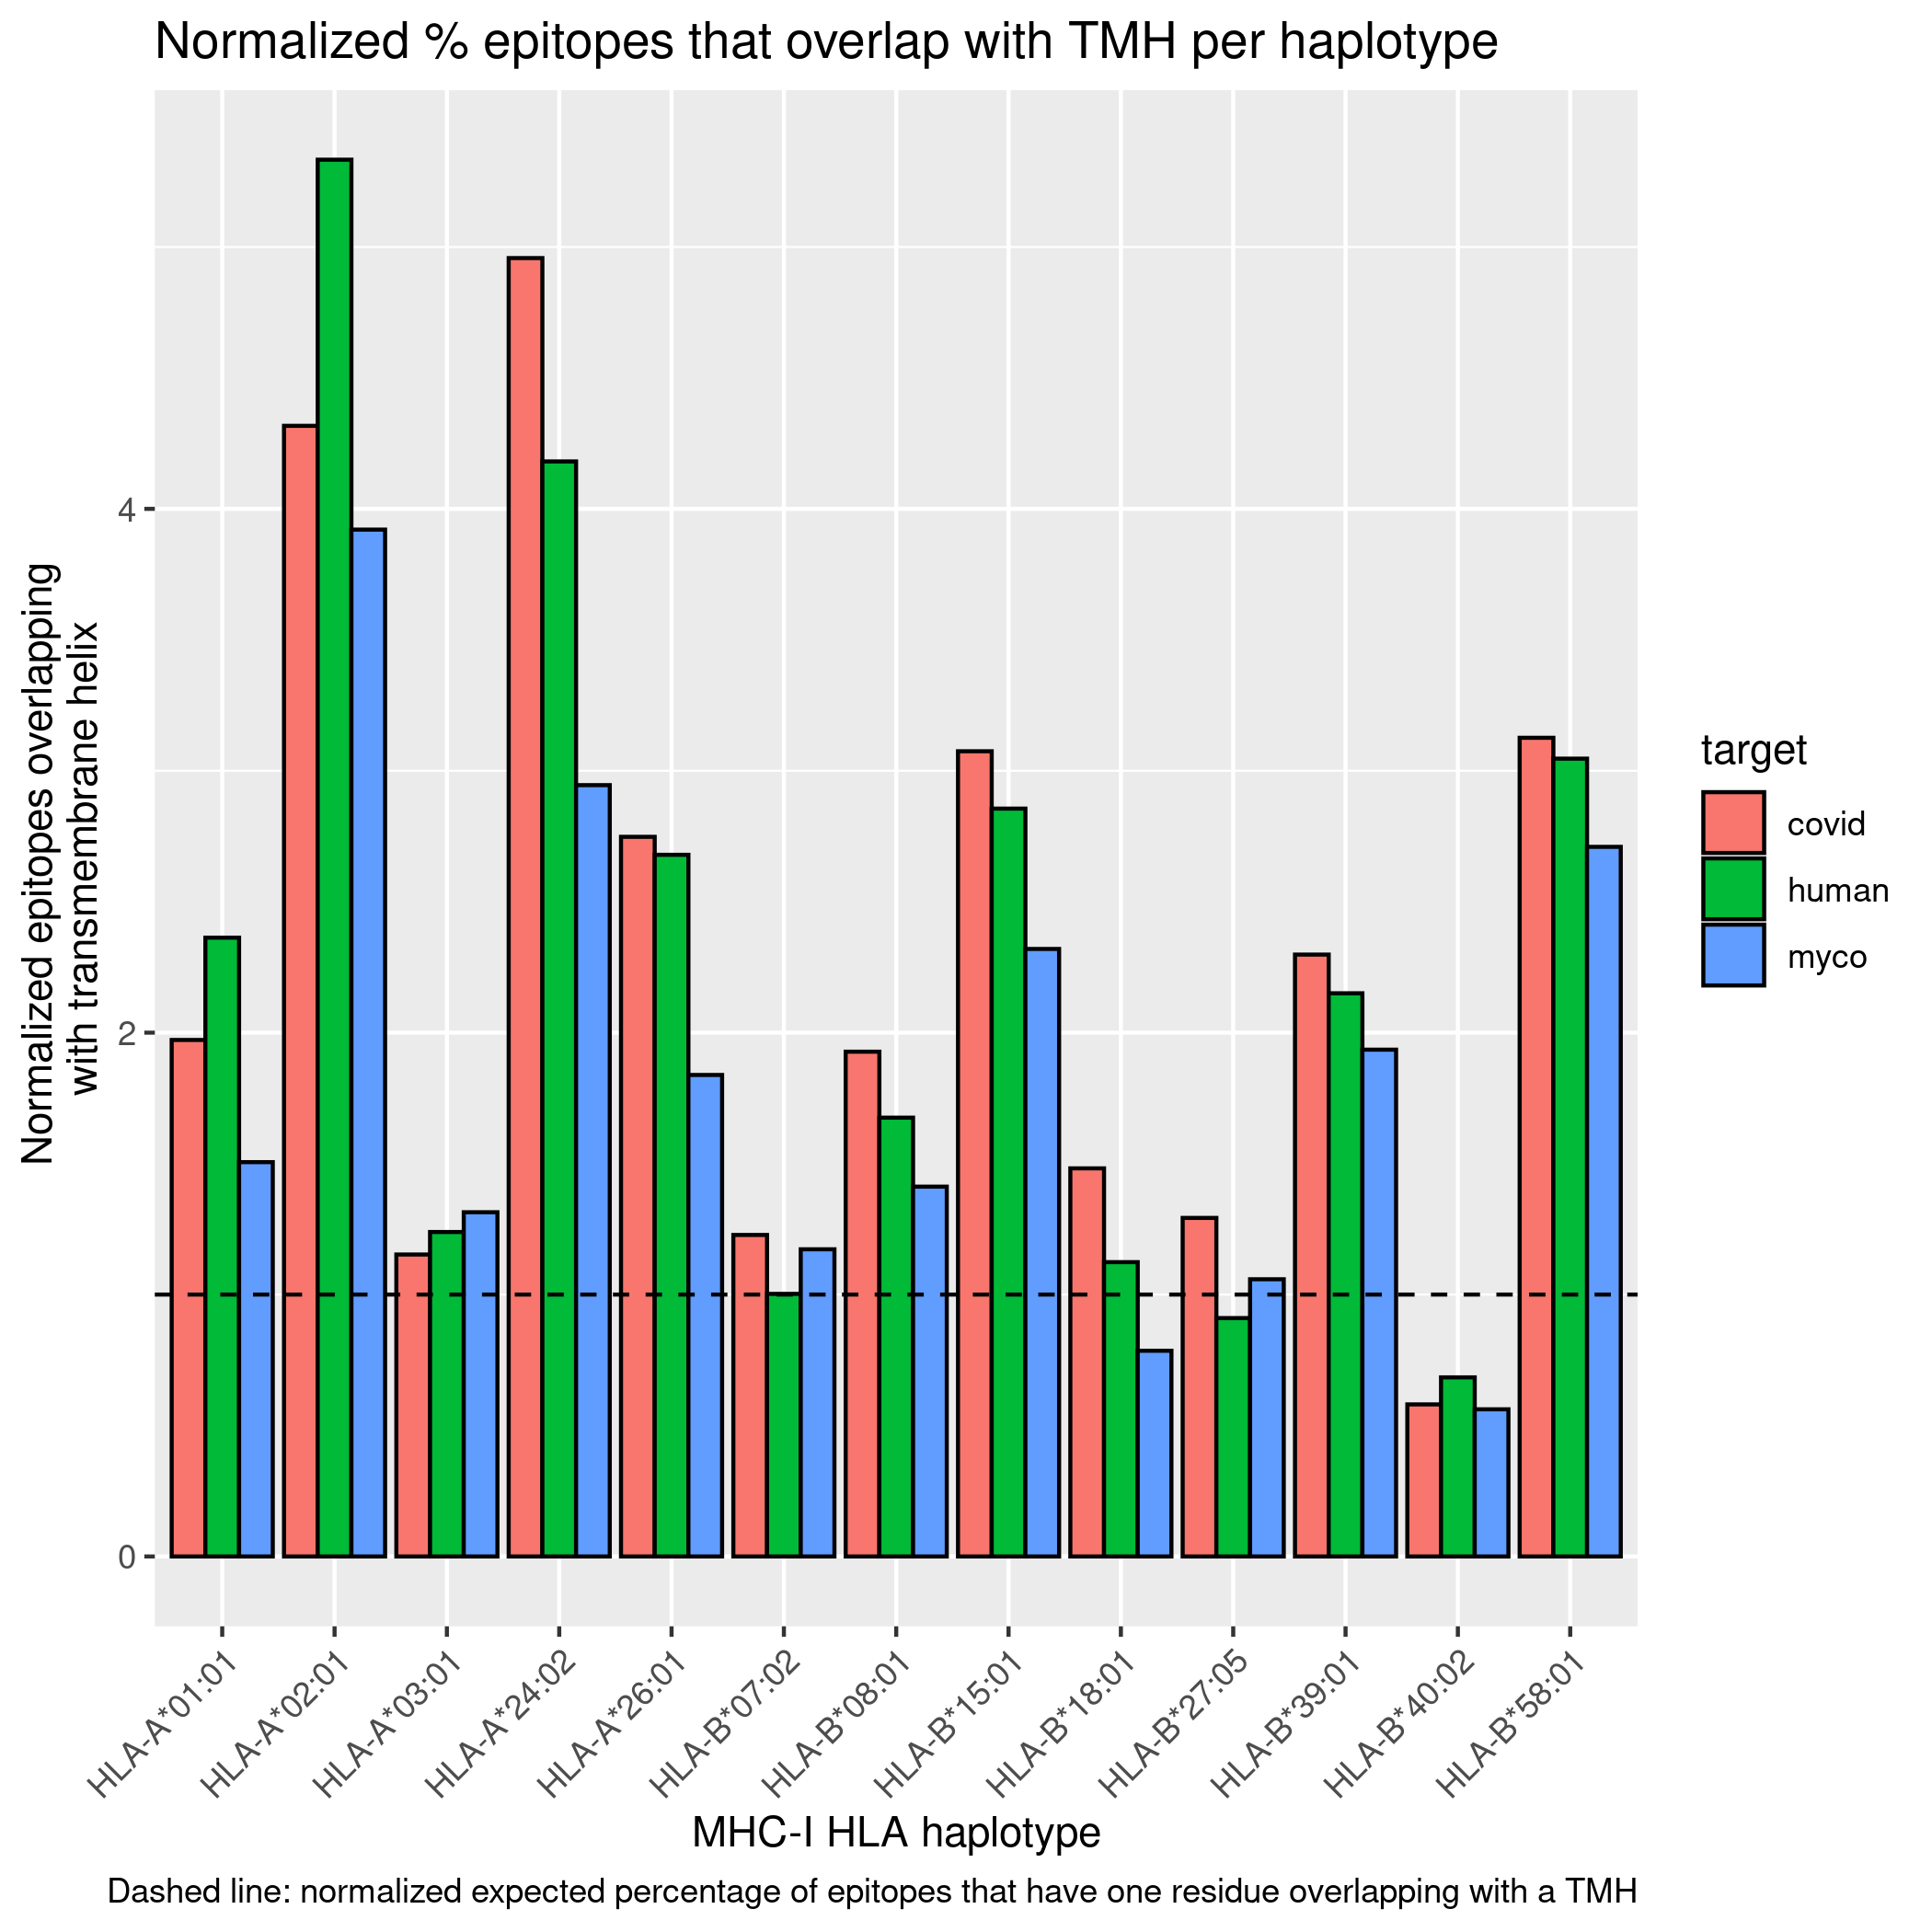
\includegraphics[width=\textwidth]{bbbq_1_smart_results/fig_f_tmh_mhc1_2_normalized.png}
  \caption{
    Normalized proportion of MHC-I epitopes overlapping with TMHs
    for human, viral and bacterial proteomes.
    Legend: covid = SARS-CoV-2,
    human = \emph{Homo sapiens}, 
    myco = \emph{Mycobacterium tuberculosis}
  }
  \label{fig:f_tmh_mhc1_normalized}
\end{figure}

\begin{figure}[!htbp]
  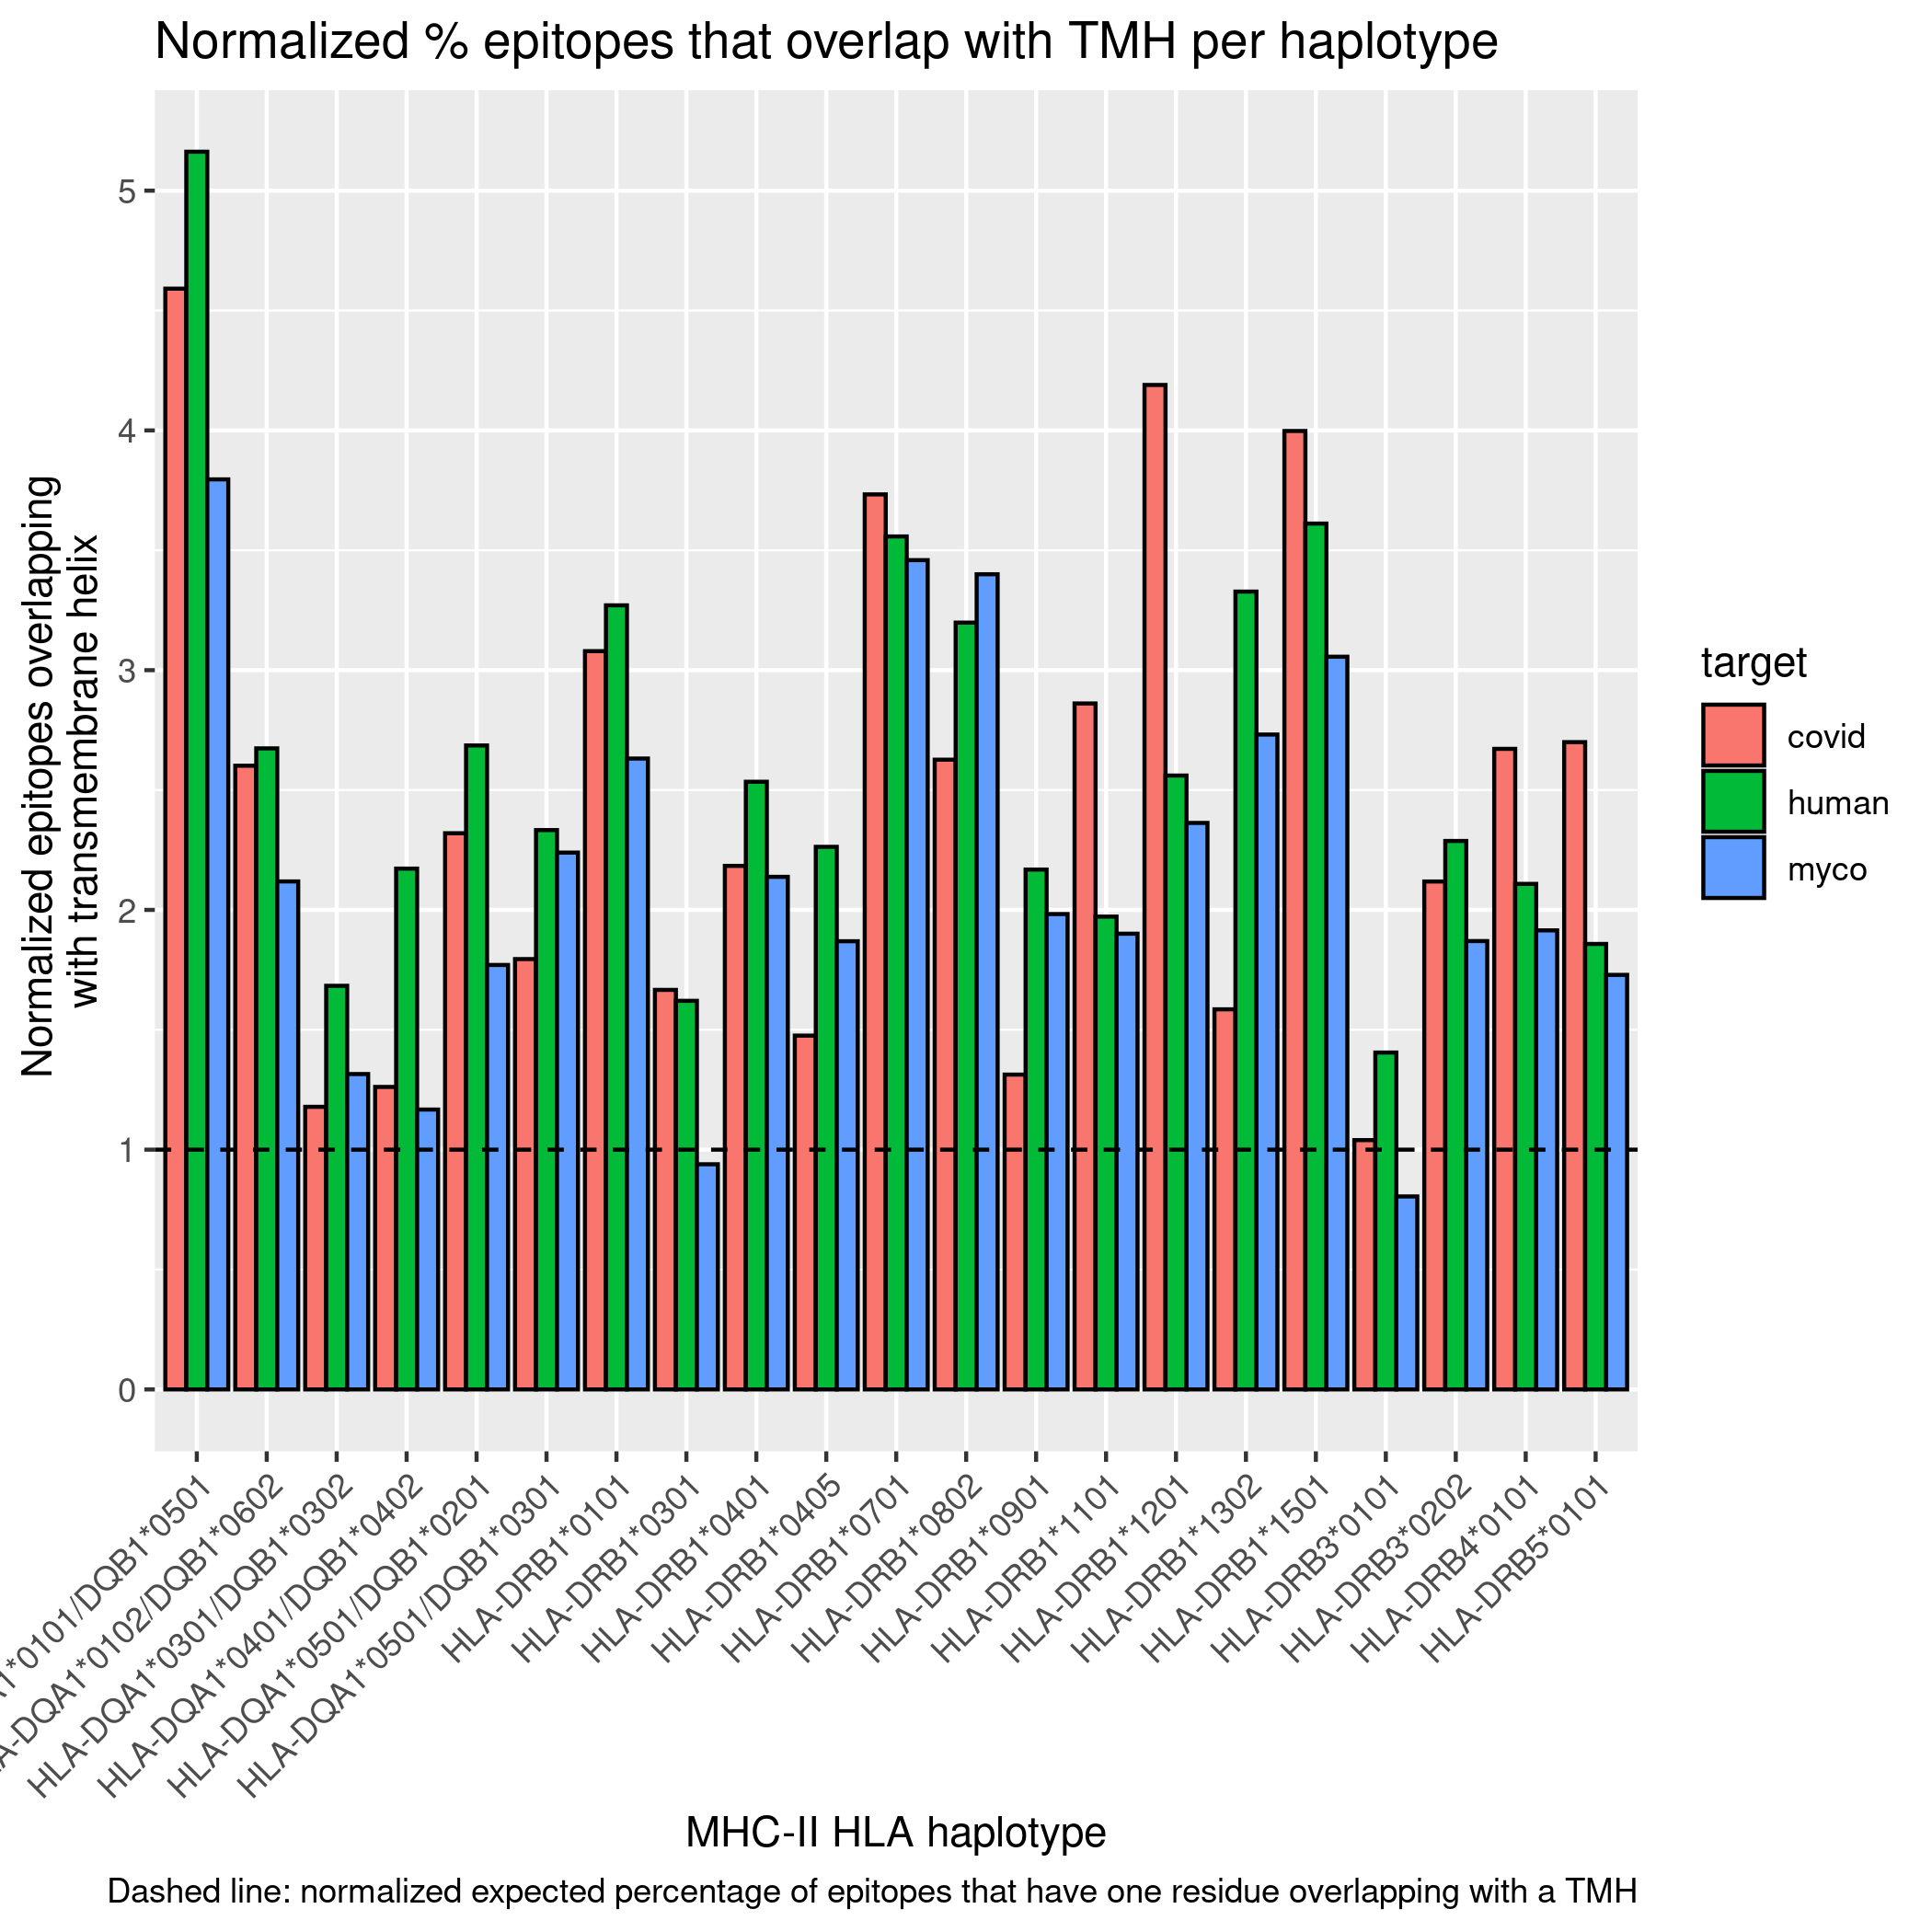
\includegraphics[width=\textwidth]{bbbq_1_smart_results/fig_f_tmh_mhc2_2_normalized.png}
  \caption{
    Normalized proportion of MHC-II epitopes overlapping with TMHs
    for human, viral and bacterial proteomes.
    Legend: covid = SARS-CoV-2,
    human = \emph{Homo sapiens}, myco = \emph{Mycobacterium tuberculosis}
  }
  \label{fig:f_tmh_mhc2_normalized}
\end{figure}

To determine the additional over-presentation of TMH-derived epitopes 
in MHC-II (as compared to MHC-I), we normalized the data to enable
a side-by-side comparison. 
The percentage of TMH-derived epitopes presented was normalized
to the expected percentage of TMH-derived epitopes,
where $1.0$ denotes that the percentage of presented TMH-derived epitopes
matches the values as expected by chance.
The normalized values per haplotype are shown 
in figure \ref{fig:rel_presentation_per_haplotype}.
To compare the TMH-derived over-presentation per MHC class,
we grouped the normalized values per haplotype, 
and plot the mean and standard error, as shown in figure \ref{fig:rel_presentation}.

\begin{figure}[!htbp]
  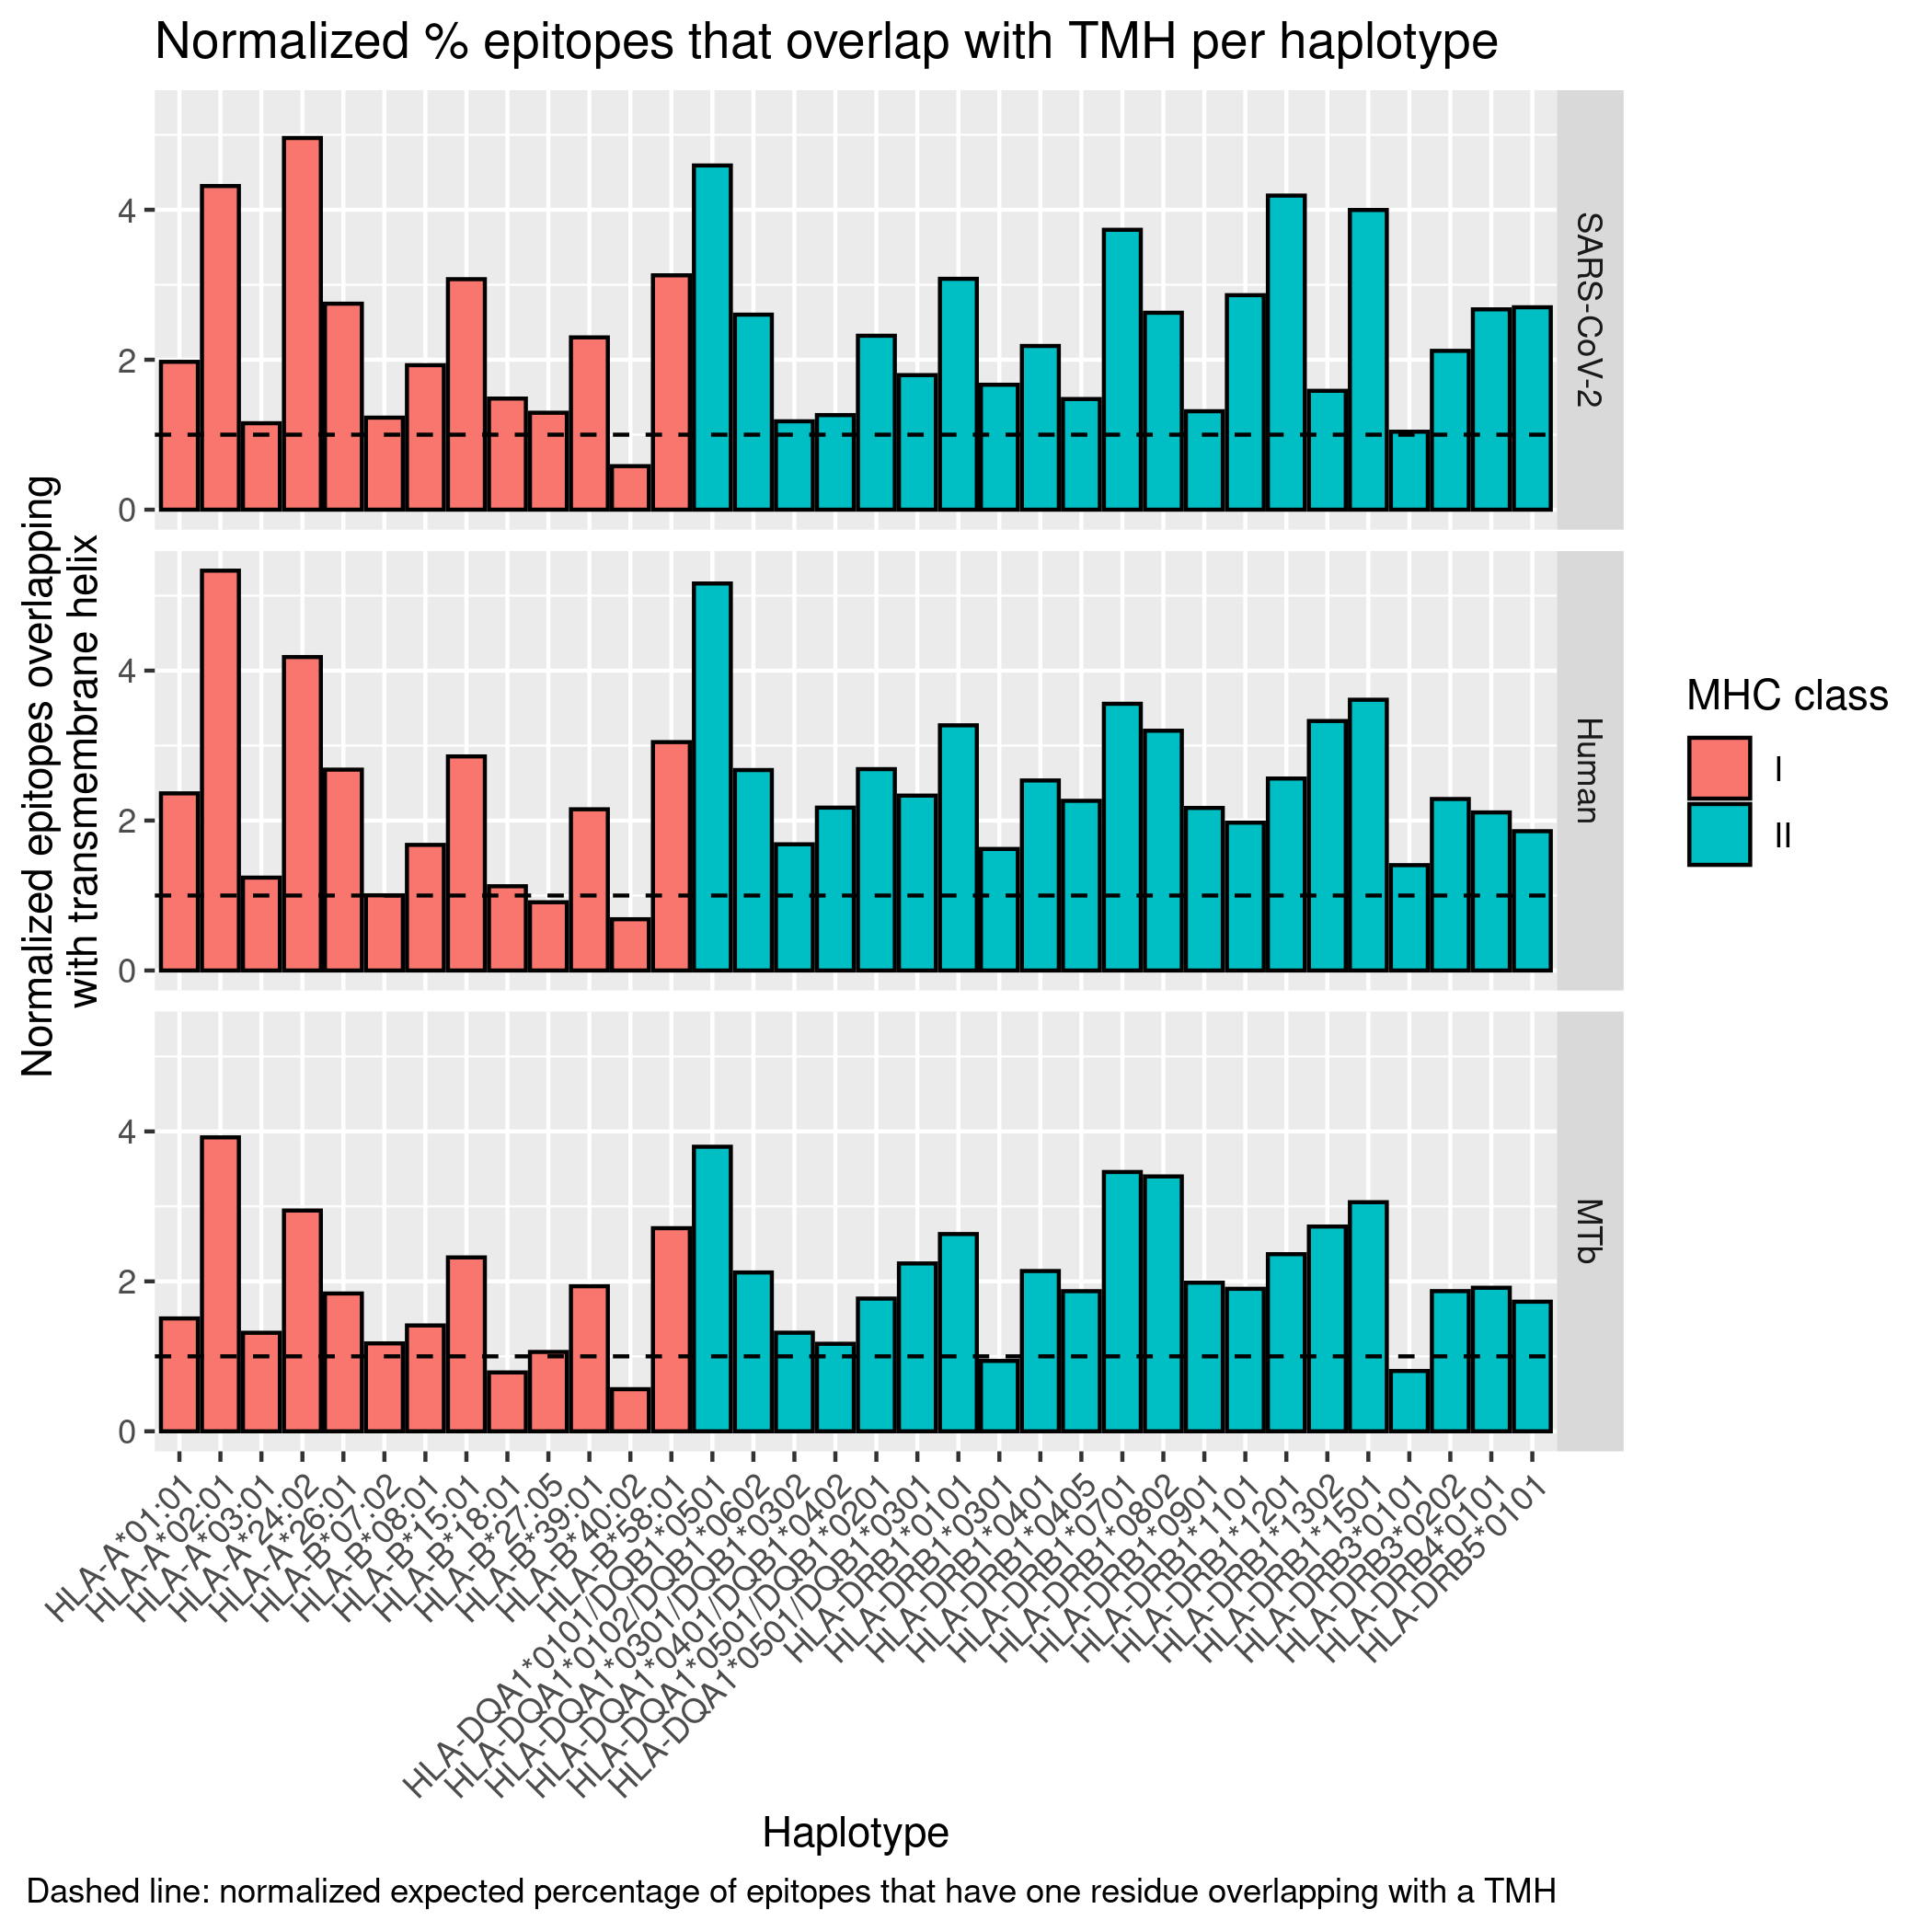
\includegraphics[width=\textwidth]{bbbq_1_smart_results/fig_rel_presentation_per_haplotype.png}
  \caption{
    Normalized proportion of MHC-I and MHC-II epitopes overlapping with TMHs,
    for the different haplotypes and proteomes
  }
  \label{fig:rel_presentation_per_haplotype}
\end{figure}

\begin{figure}[!htbp]
  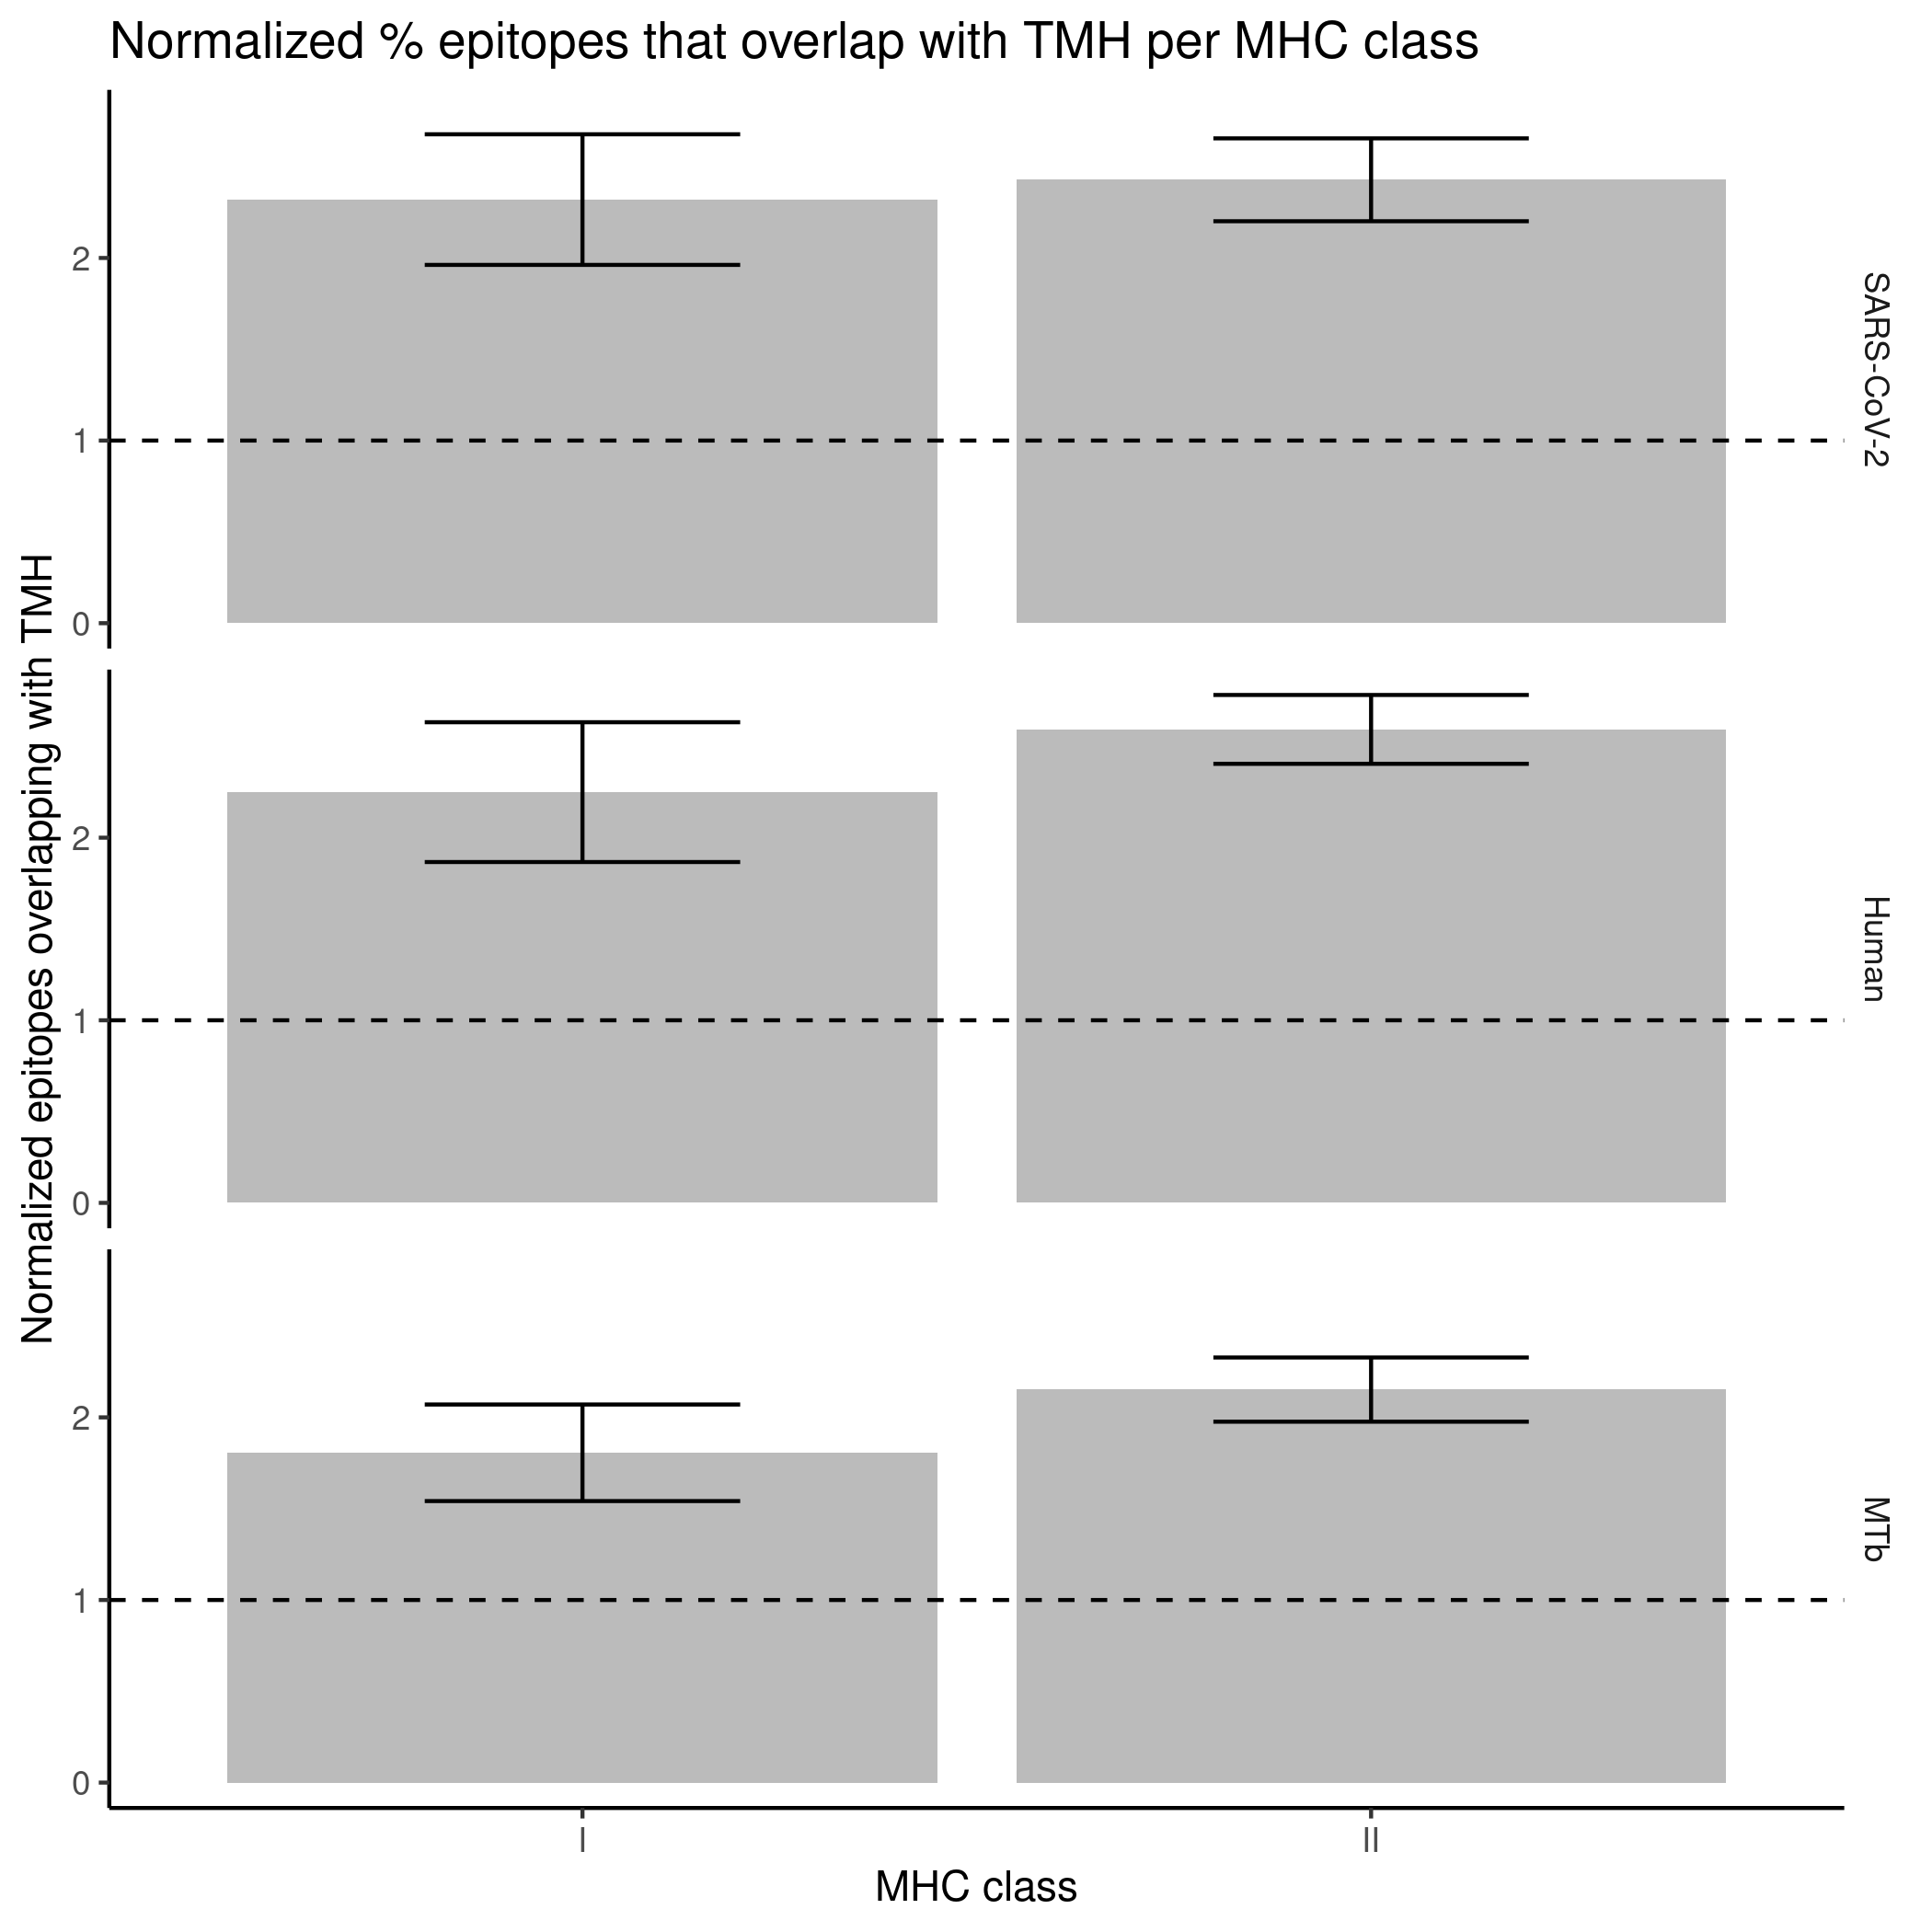
\includegraphics[width=\textwidth]{bbbq_1_smart_results/fig_rel_presentation.png}
  \caption{
    Normalized proportion of MHC-I and MHC-II epitopes overlapping with TMHs,
    for the different MHC classes and proteomes. Error bars denote the
    standard error.
  }
  \label{fig:rel_presentation}
\end{figure}

% Process all floats before going to a next page
\clearpage

%%%%%%%%%%%%%%%%%%%%%%%%%%%%%%%%%%%%%%%%%%%%%%%%%%%%%%%%%%%%%%%%%%%%%%%%%%%%%%%%
\subsection{Evolutionary conservation}
%%%%%%%%%%%%%%%%%%%%%%%%%%%%%%%%%%%%%%%%%%%%%%%%%%%%%%%%%%%%%%%%%%%%%%%%%%%%%%%%

Figure \ref{fig:snps_per_gene_name_ncbi} shows the distribution of the
number of SNPs per gene name, at the date we started the experiment,
at December 14th 2020.

\begin{figure}[!htbp]
  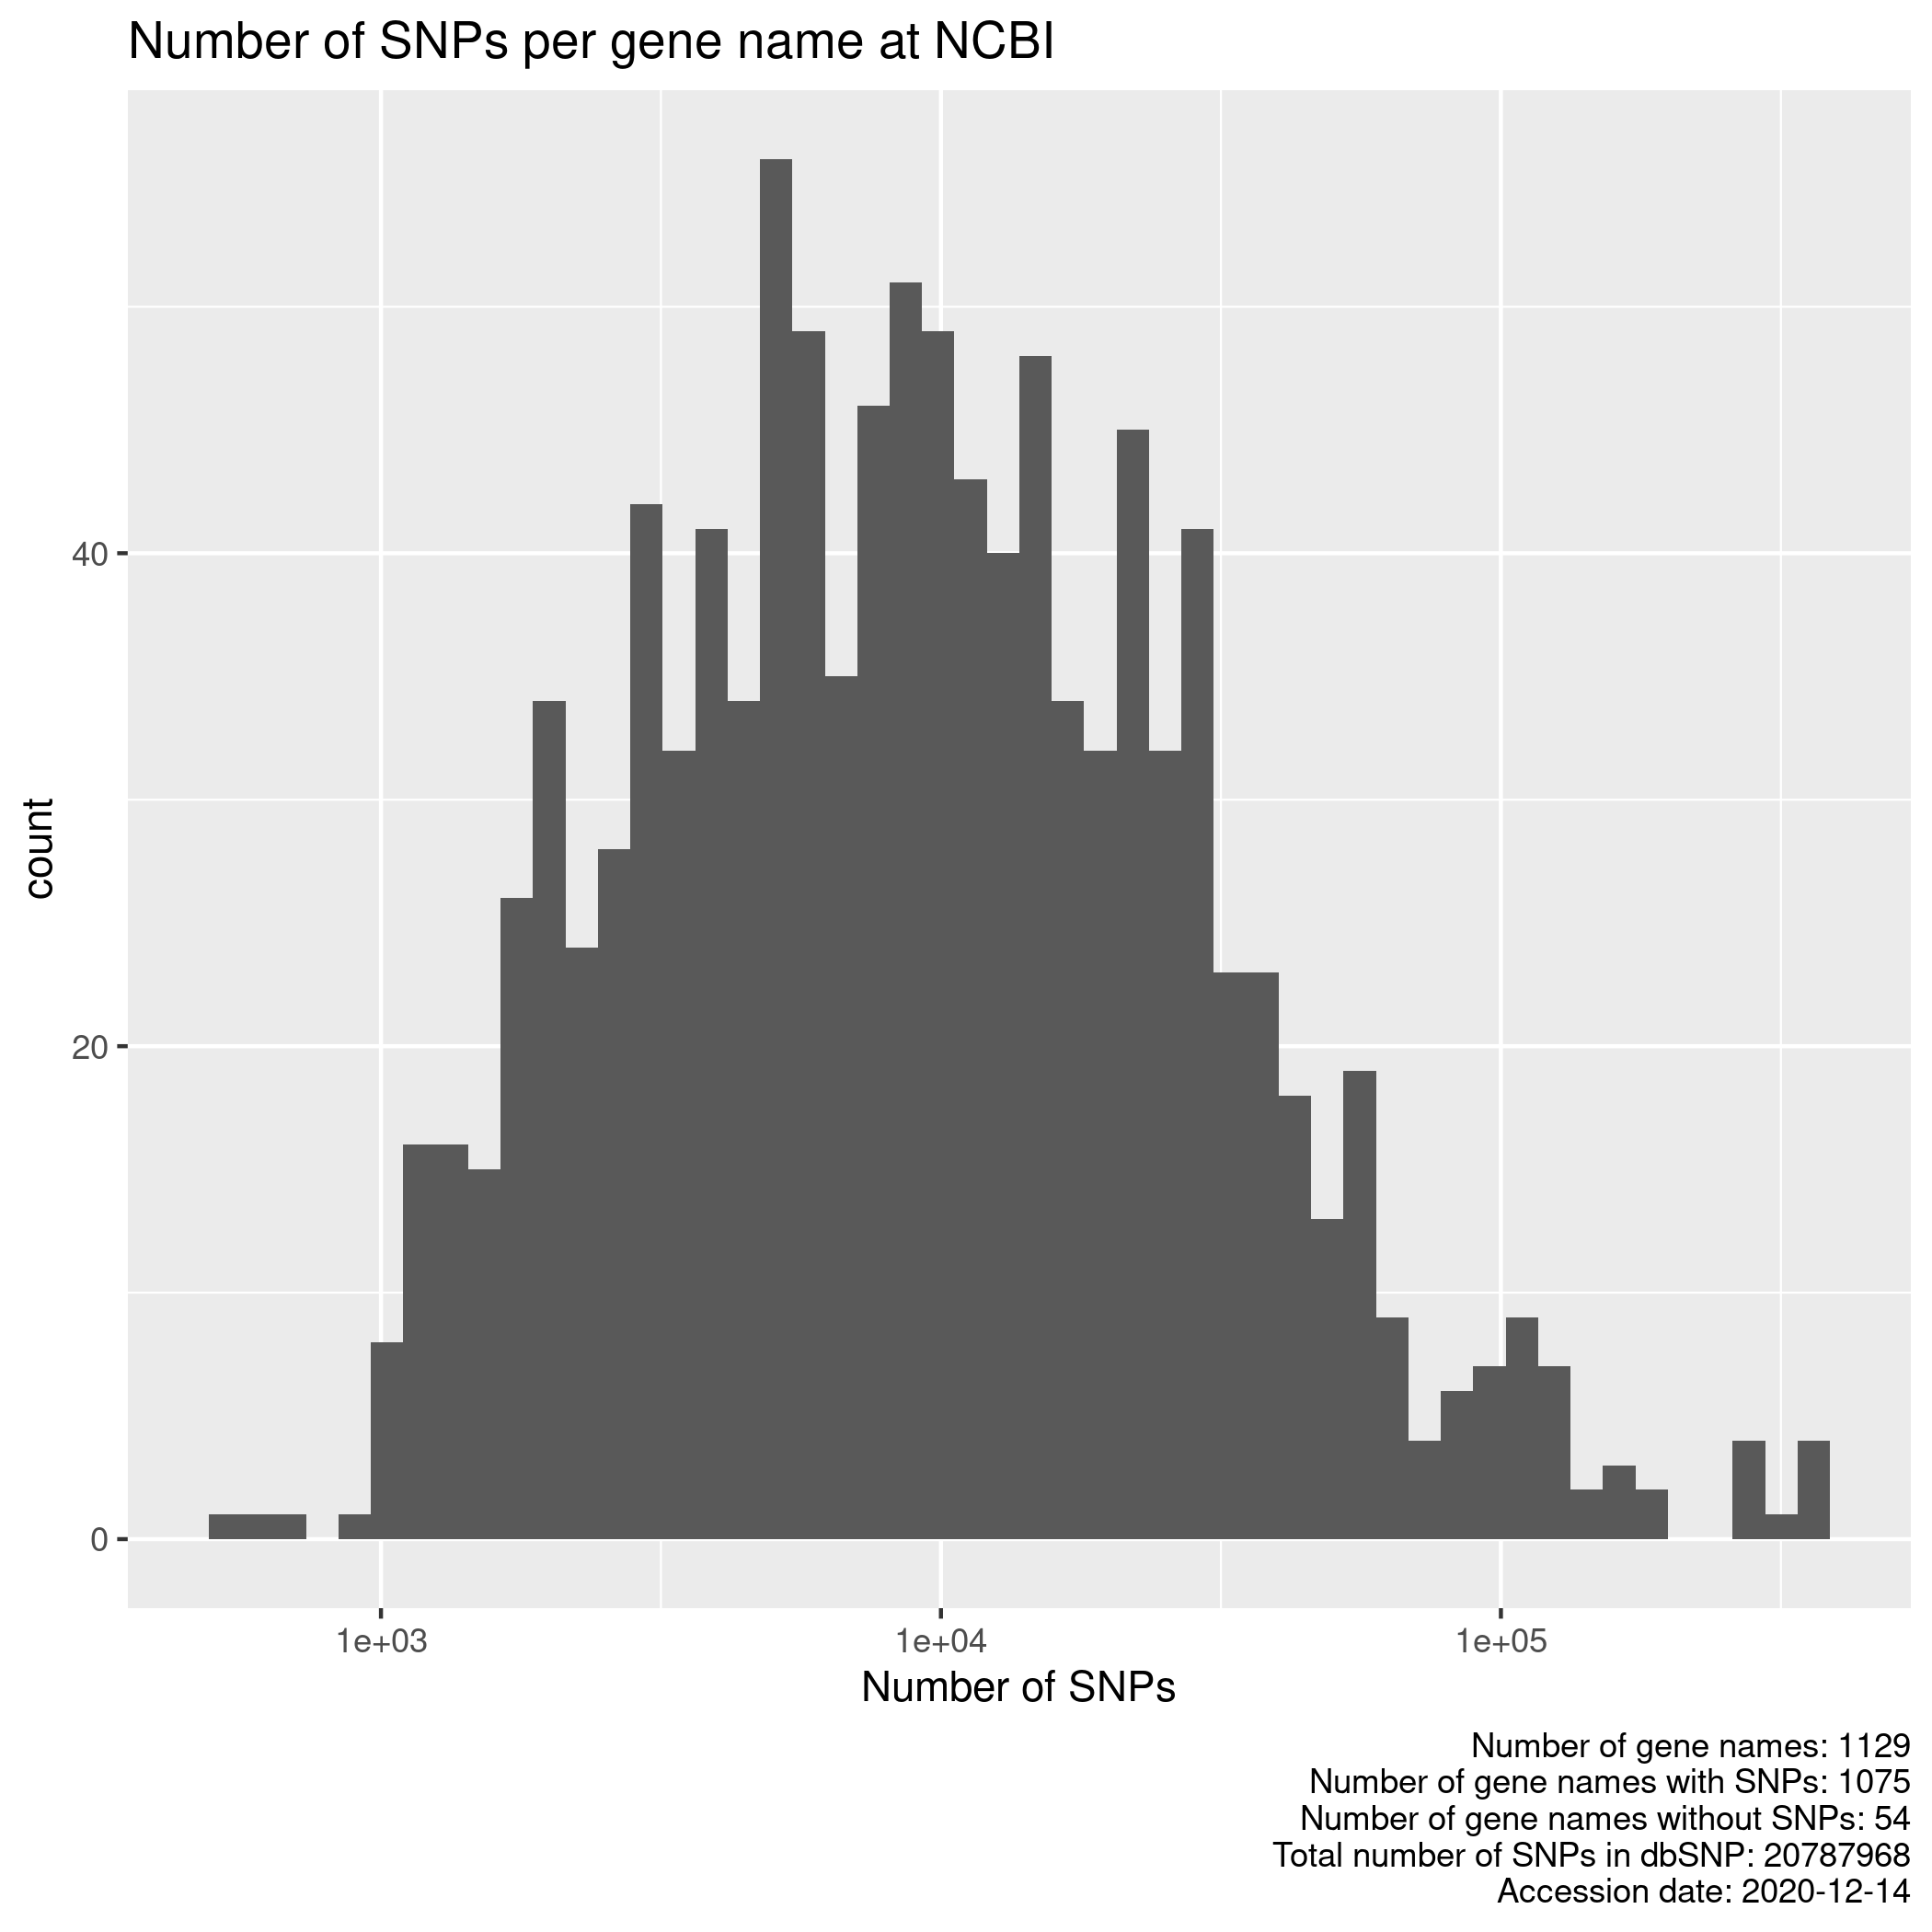
\includegraphics[width=\textwidth]{ncbi_peregrine_results/fig_snps_per_gene_name_ncbi.png}
  \caption{
    Distribution of the number of SNPs per gene name in the NCBI database.
  }
  \label{fig:snps_per_gene_name_ncbi}
\end{figure}

\begin{figure}[!htbp]
  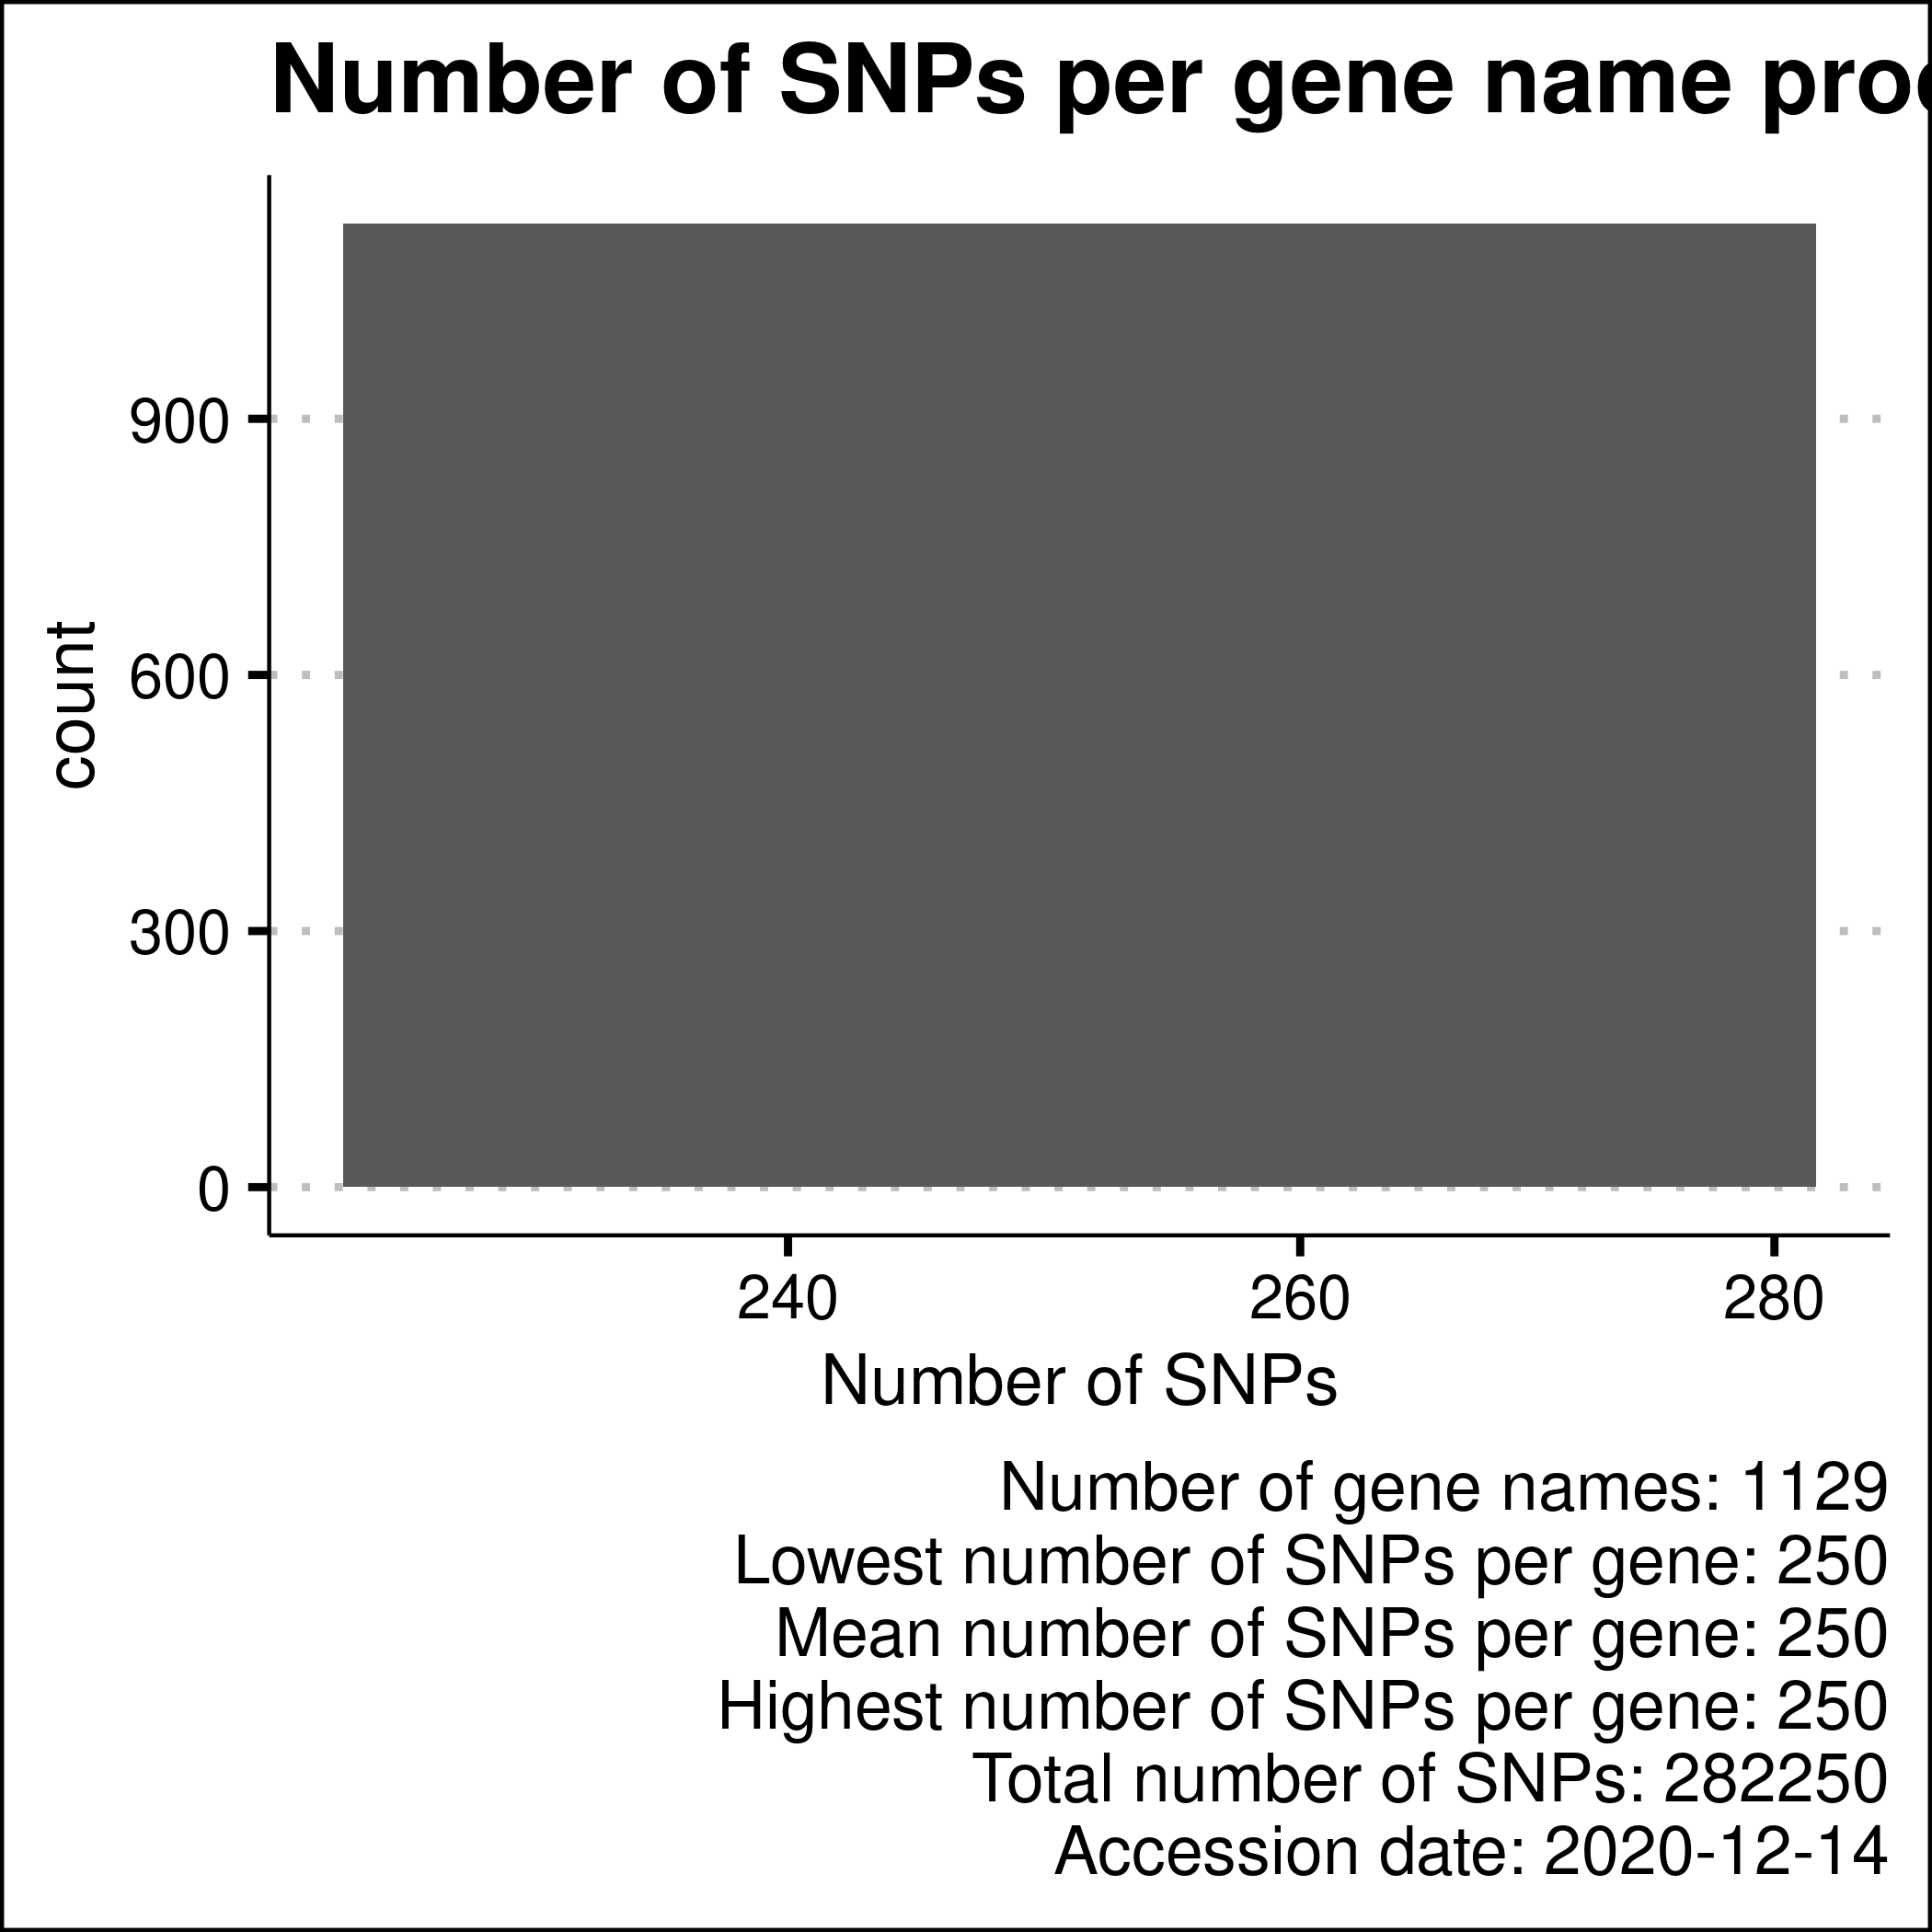
\includegraphics[width=\textwidth]{ncbi_peregrine_results/fig_snps_per_gene_name_processed.png}
  \caption{
    Distribution of the number of protein variations and SNPs per gene name processed.
  }
  \label{fig:snps_per_gene_name_processed}
\end{figure}

\begin{figure}[!htbp]
  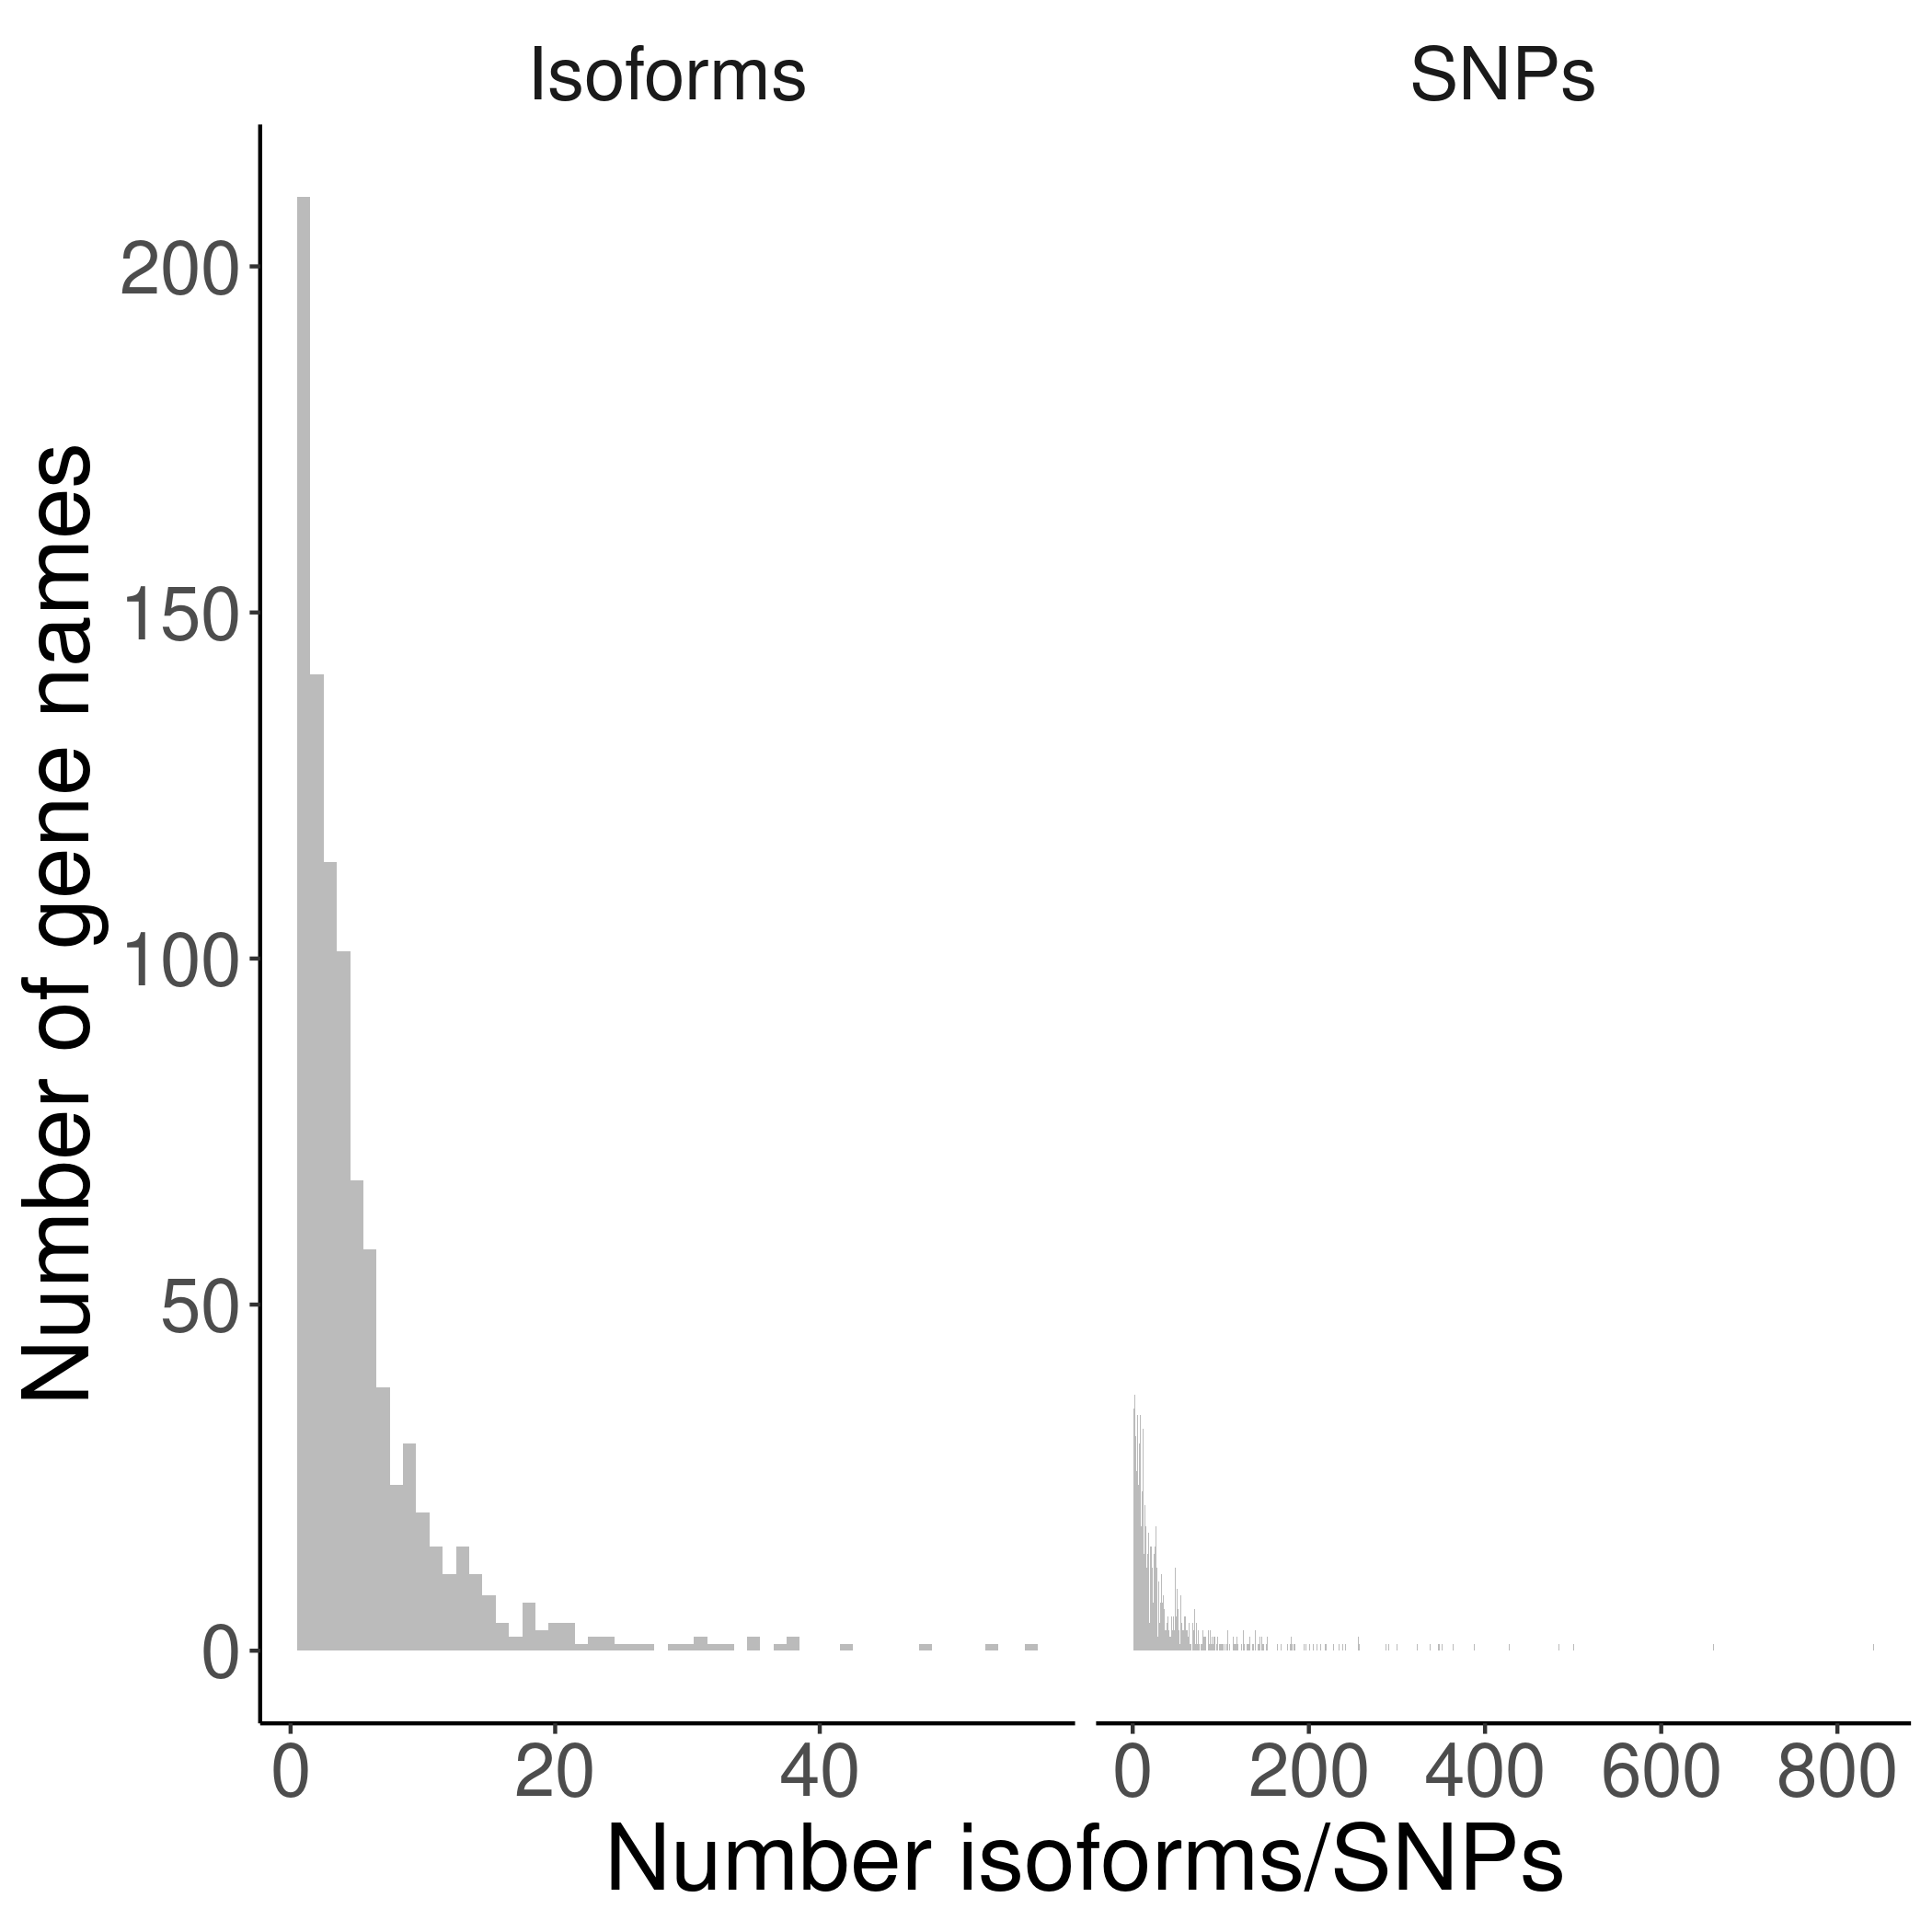
\includegraphics[width=\textwidth]{ncbi_peregrine_results/fig_n_proteins_per_gene_name.png}
  \caption{
    Histogram of the number of proteins found per gene name.
    Most often, a gene name is associated with one proteins. 
  }
  \label{fig:n_proteins_per_gene_name}
\end{figure}


\begin{figure}[!htbp]
  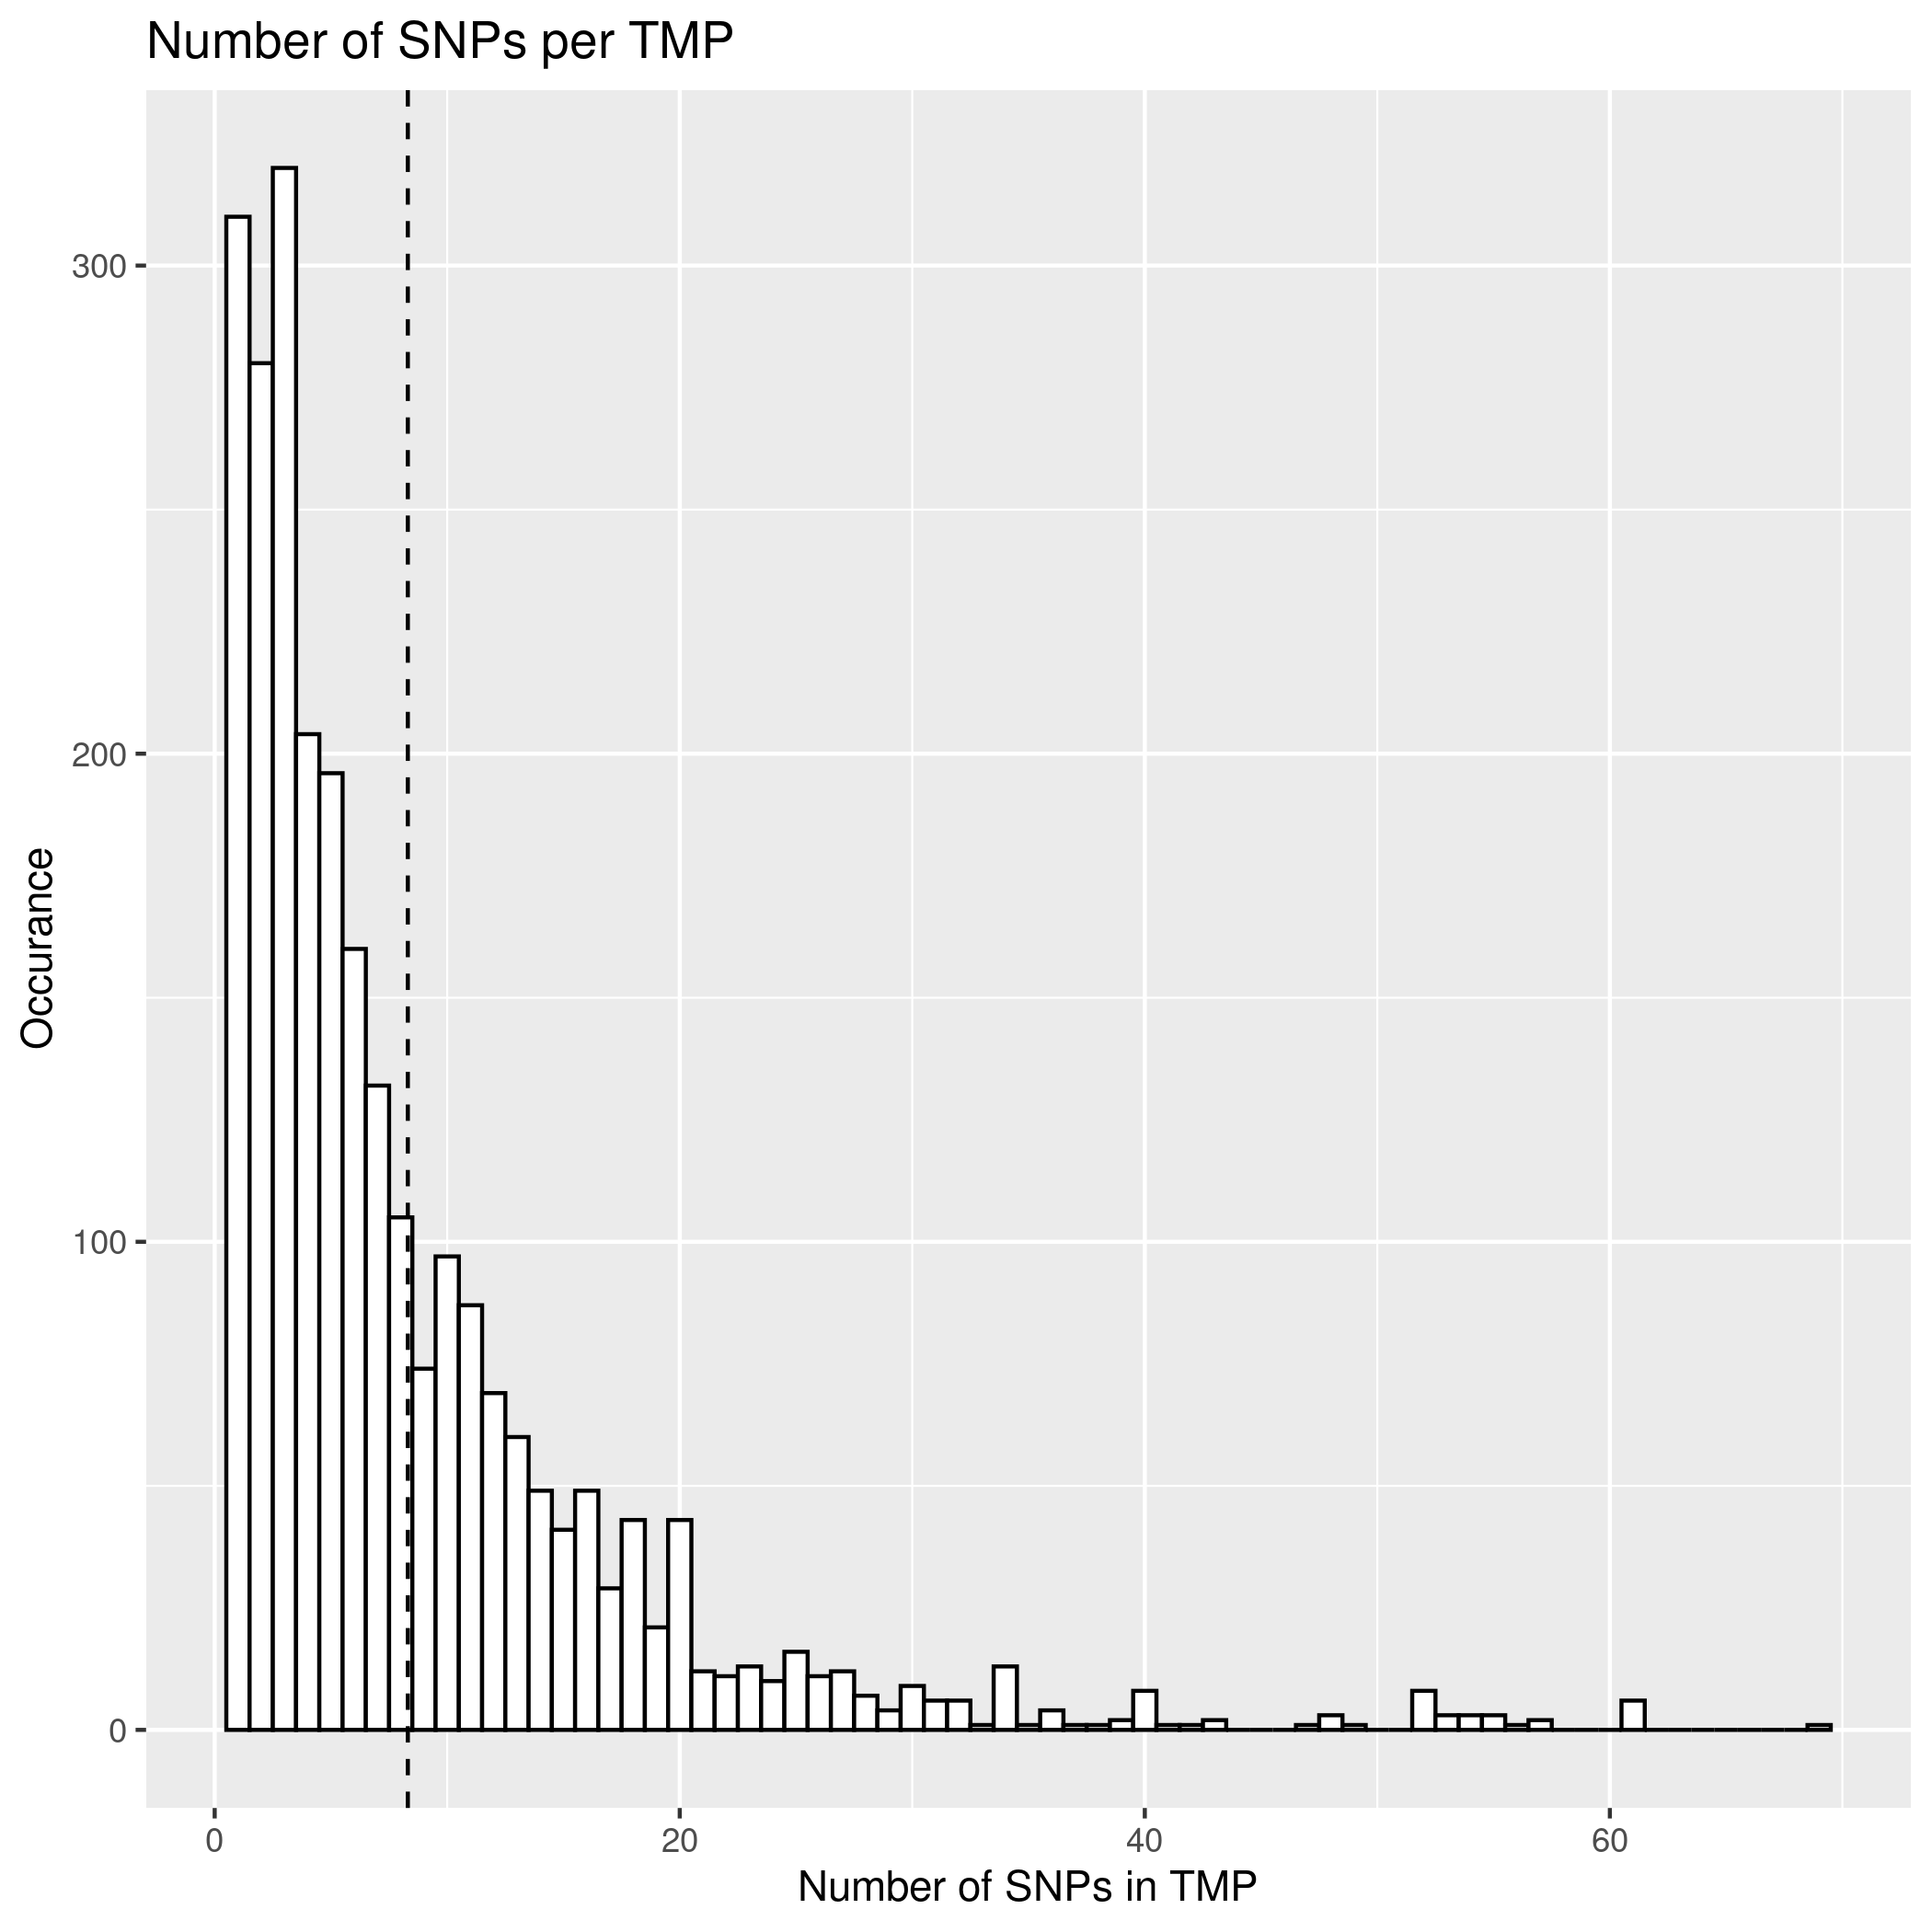
\includegraphics[width=\textwidth]{ncbi_peregrine_results/fig_n_snps_per_tmp.png}
  \caption{
    Histogram of the number of SNPs per trans-membrane protein.
    Dashed vertical line: average number of SNPs per TMP
  }
  \label{fig:fig_n_snps_per_tmp}
\end{figure}

\begin{figure}[!htbp]
  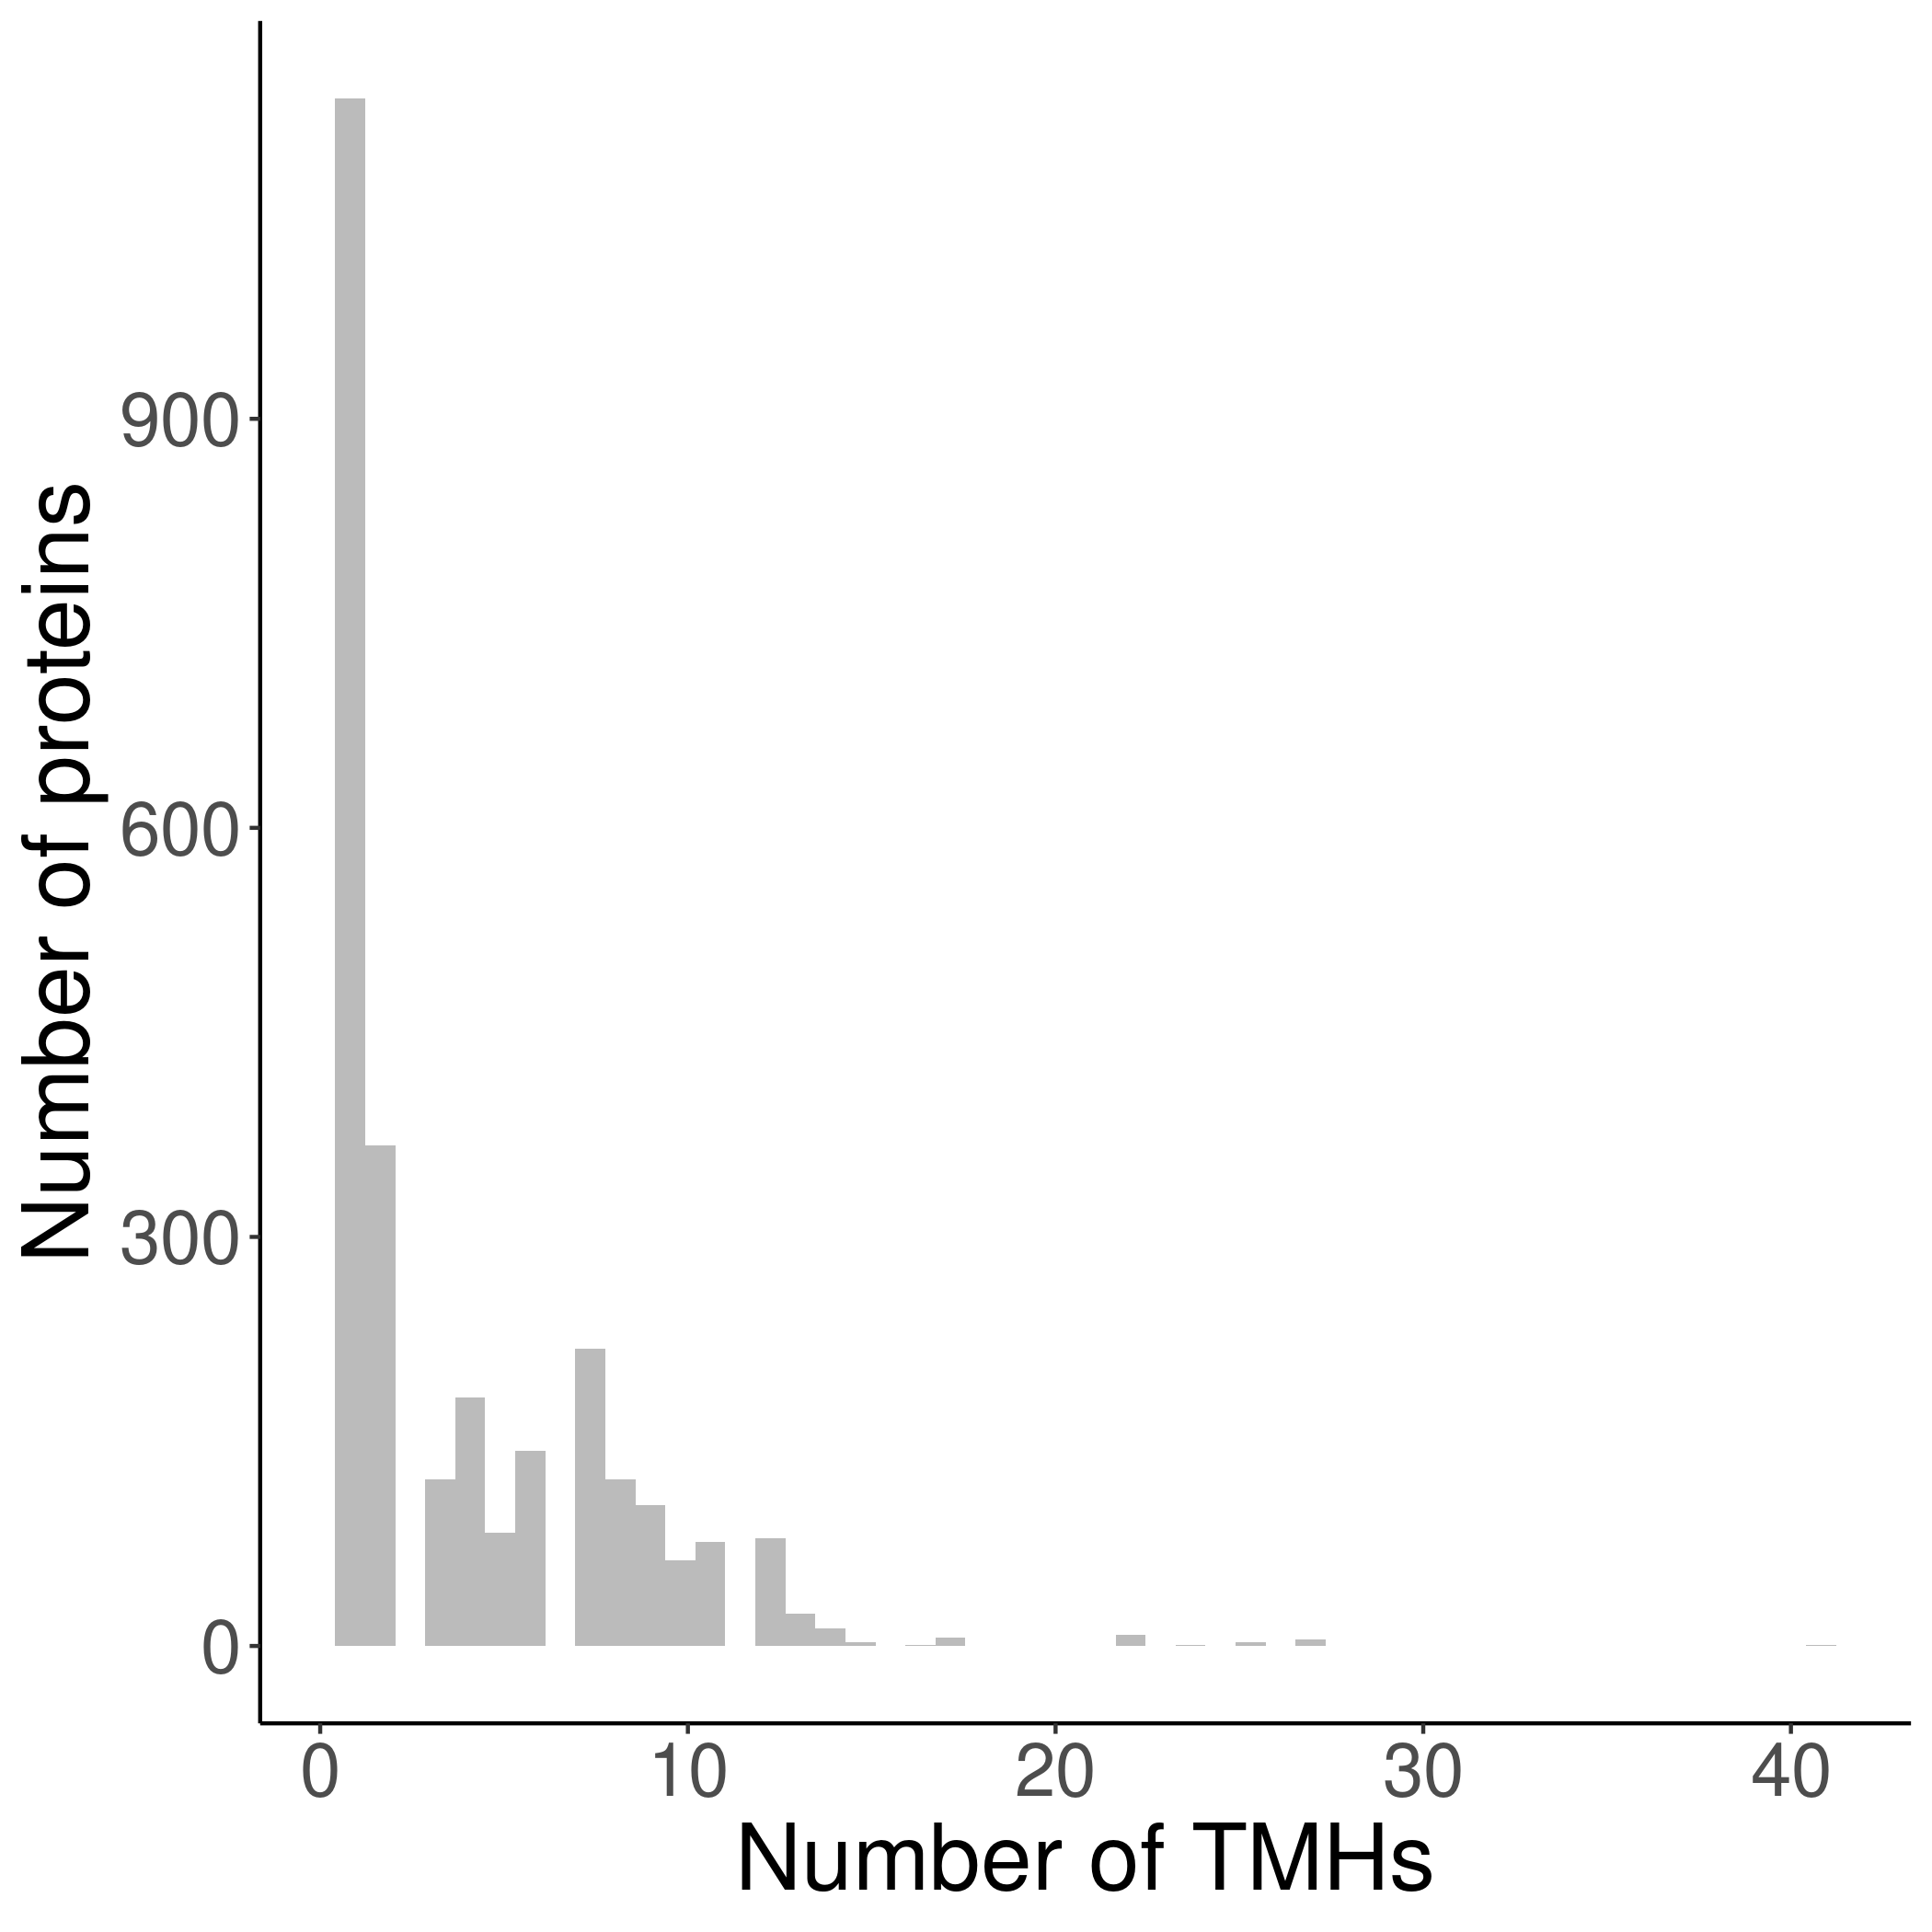
\includegraphics[width=\textwidth]{ncbi_peregrine_results/fig_n_tmhs_per_protein.png}
  \caption{
    Histogram of the number of TMHs predicted per protein,
    for the trans-membrane proteins used.
  }
  \label{fig:fig_n_tmhs_per_protein}
\end{figure}


% \paragraph{Relative position of SNPs}

To verify if SNPs were sampled uniformly
over proteins, we show the distribution 
of the relative position in figure \ref{fig:snp_rel_pos}.
We find no clear evidence of a bias.

% \paragraph{Statistics}

Supplementary Table \ref{tab:snp_stats} shows the statistics for all
SNPs, where supplementary Tables \ref{tab:snp_stats_per_spanner_single}
and \ref{tab:snp_stats_per_spanner_multi} show the
statistics for only single-spanners and multi-spanners respectively.
 
% Label: tab:snp_stats
\begin{table}

\caption{\label{tab:snp_stats}Statistics for the multi-spanners. p = p value. n = number of SNPs. n\_success = number of SNPs found in TMHs (dashed blue line). E(n\_success) = expected number of SNPs to be found in TMHs (dashed red line). }
\centering
\begin{tabular}[t]{l|l}
\hline
parameter & value\\
\hline
p & 6.820823e-11\\
\hline
n & 21208\\
\hline
n\_success & 3803\\
\hline
E(n\_success) & 4140.56\\
\hline
\end{tabular}
\end{table}

% Label: tab:snp_stats_per_spanner_single
\begin{table}

\caption{\label{tab:snp_stats_per_spanner_single}Statistics for the single-spanners. p = p value. n = number of SNPs in single-spanners. n\_success = number of SNPs found in TMHs of single-spanners (dashed blue line). E(n\_success) = expected number of SNPs to be found in TMHs of single-spanners. }
\centering
\begin{tabular}[t]{l|l}
\hline
parameter & value\\
\hline
p & 0.3189532\\
\hline
n & 8186\\
\hline
n\_success & 452\\
\hline
E(n\_success) & 462.1535\\
\hline
\end{tabular}
\end{table}


% Label: tab:snp_stats_per_spanner_multi
\begin{table}

\caption{\label{tab:snp_stats_per_spanner_multi}Statistics for the multi-spanners. p = p value. n = number of SNPs in multi-spanners. n\_success = number of SNPs found in TMHs of multi-spanners (dashed blue line). E(n\_success) = expected number of SNPs to be found in TMHs of multi-spanners  (dashed red line). }
\centering
\begin{tabular}[t]{l|l}
\hline
parameter & value\\
\hline
p & 4.388709e-14\\
\hline
n & 13386\\
\hline
n\_success & 3377\\
\hline
E(n\_success) & 3767.26\\
\hline
\end{tabular}
\end{table}

% Process all floats before going to a next page
\clearpage

%%%%%%%%%%%%%%%%%%%%%%%%%%%%%%%%%%%%%%%%%%%%%%%%%%%%%%%%%%%%%%%%%%%%%%%%%%%%%%%%
\subsection{Presentation of TMH-derived epitopes when two amino acids overlap}
%%%%%%%%%%%%%%%%%%%%%%%%%%%%%%%%%%%%%%%%%%%%%%%%%%%%%%%%%%%%%%%%%%%%%%%%%%%%%%%%

In our experiment, we define a TMH-derived epitope as a peptide that overlaps
with a TMH for at least one amino acid. One could argue that we should use
a higher number of overlapping amino acids, so to make the epitopes more
'transmembrane helix-ey'. We chose not too, for two reason: (1) epitopes that overlap with a TMH
for 1 AA already, cannot be processed by the proteasome in a known and conventional
way (2) whatever number of overlapping amino acids we use, we expect the pattern to be the same.
However, using only 1 AA gives the most TMH-derived epitopes and hence the highest statistical
power.

To prove this point, we did exactly the same analysis 
as shown in Figure \ref{fig:bbbq_1_smart_results},
yet with defining a TMH-derived epitope as an epitope that overlaps with a TMH
for at least 2 AAs, as shown in Figure \ref{fig:bbbq_1_smart_results_2aas}.
As these two figures look identical, 
we also added the counts as numbers,
with Table \ref{tab:tmh_binders_mhc2_2aas} showing the same data
as \ref{tab:tmh_binders_mhc2}, except the former uses 2 AAs overlap.
Likewise, Table \ref{tab:tmh_binders_mhc1_2aas} showing the same data
as \ref{tab:tmh_binders_mhc1}, except the former uses 2 AAs overlap.

\begin{figure}[!htbp]
  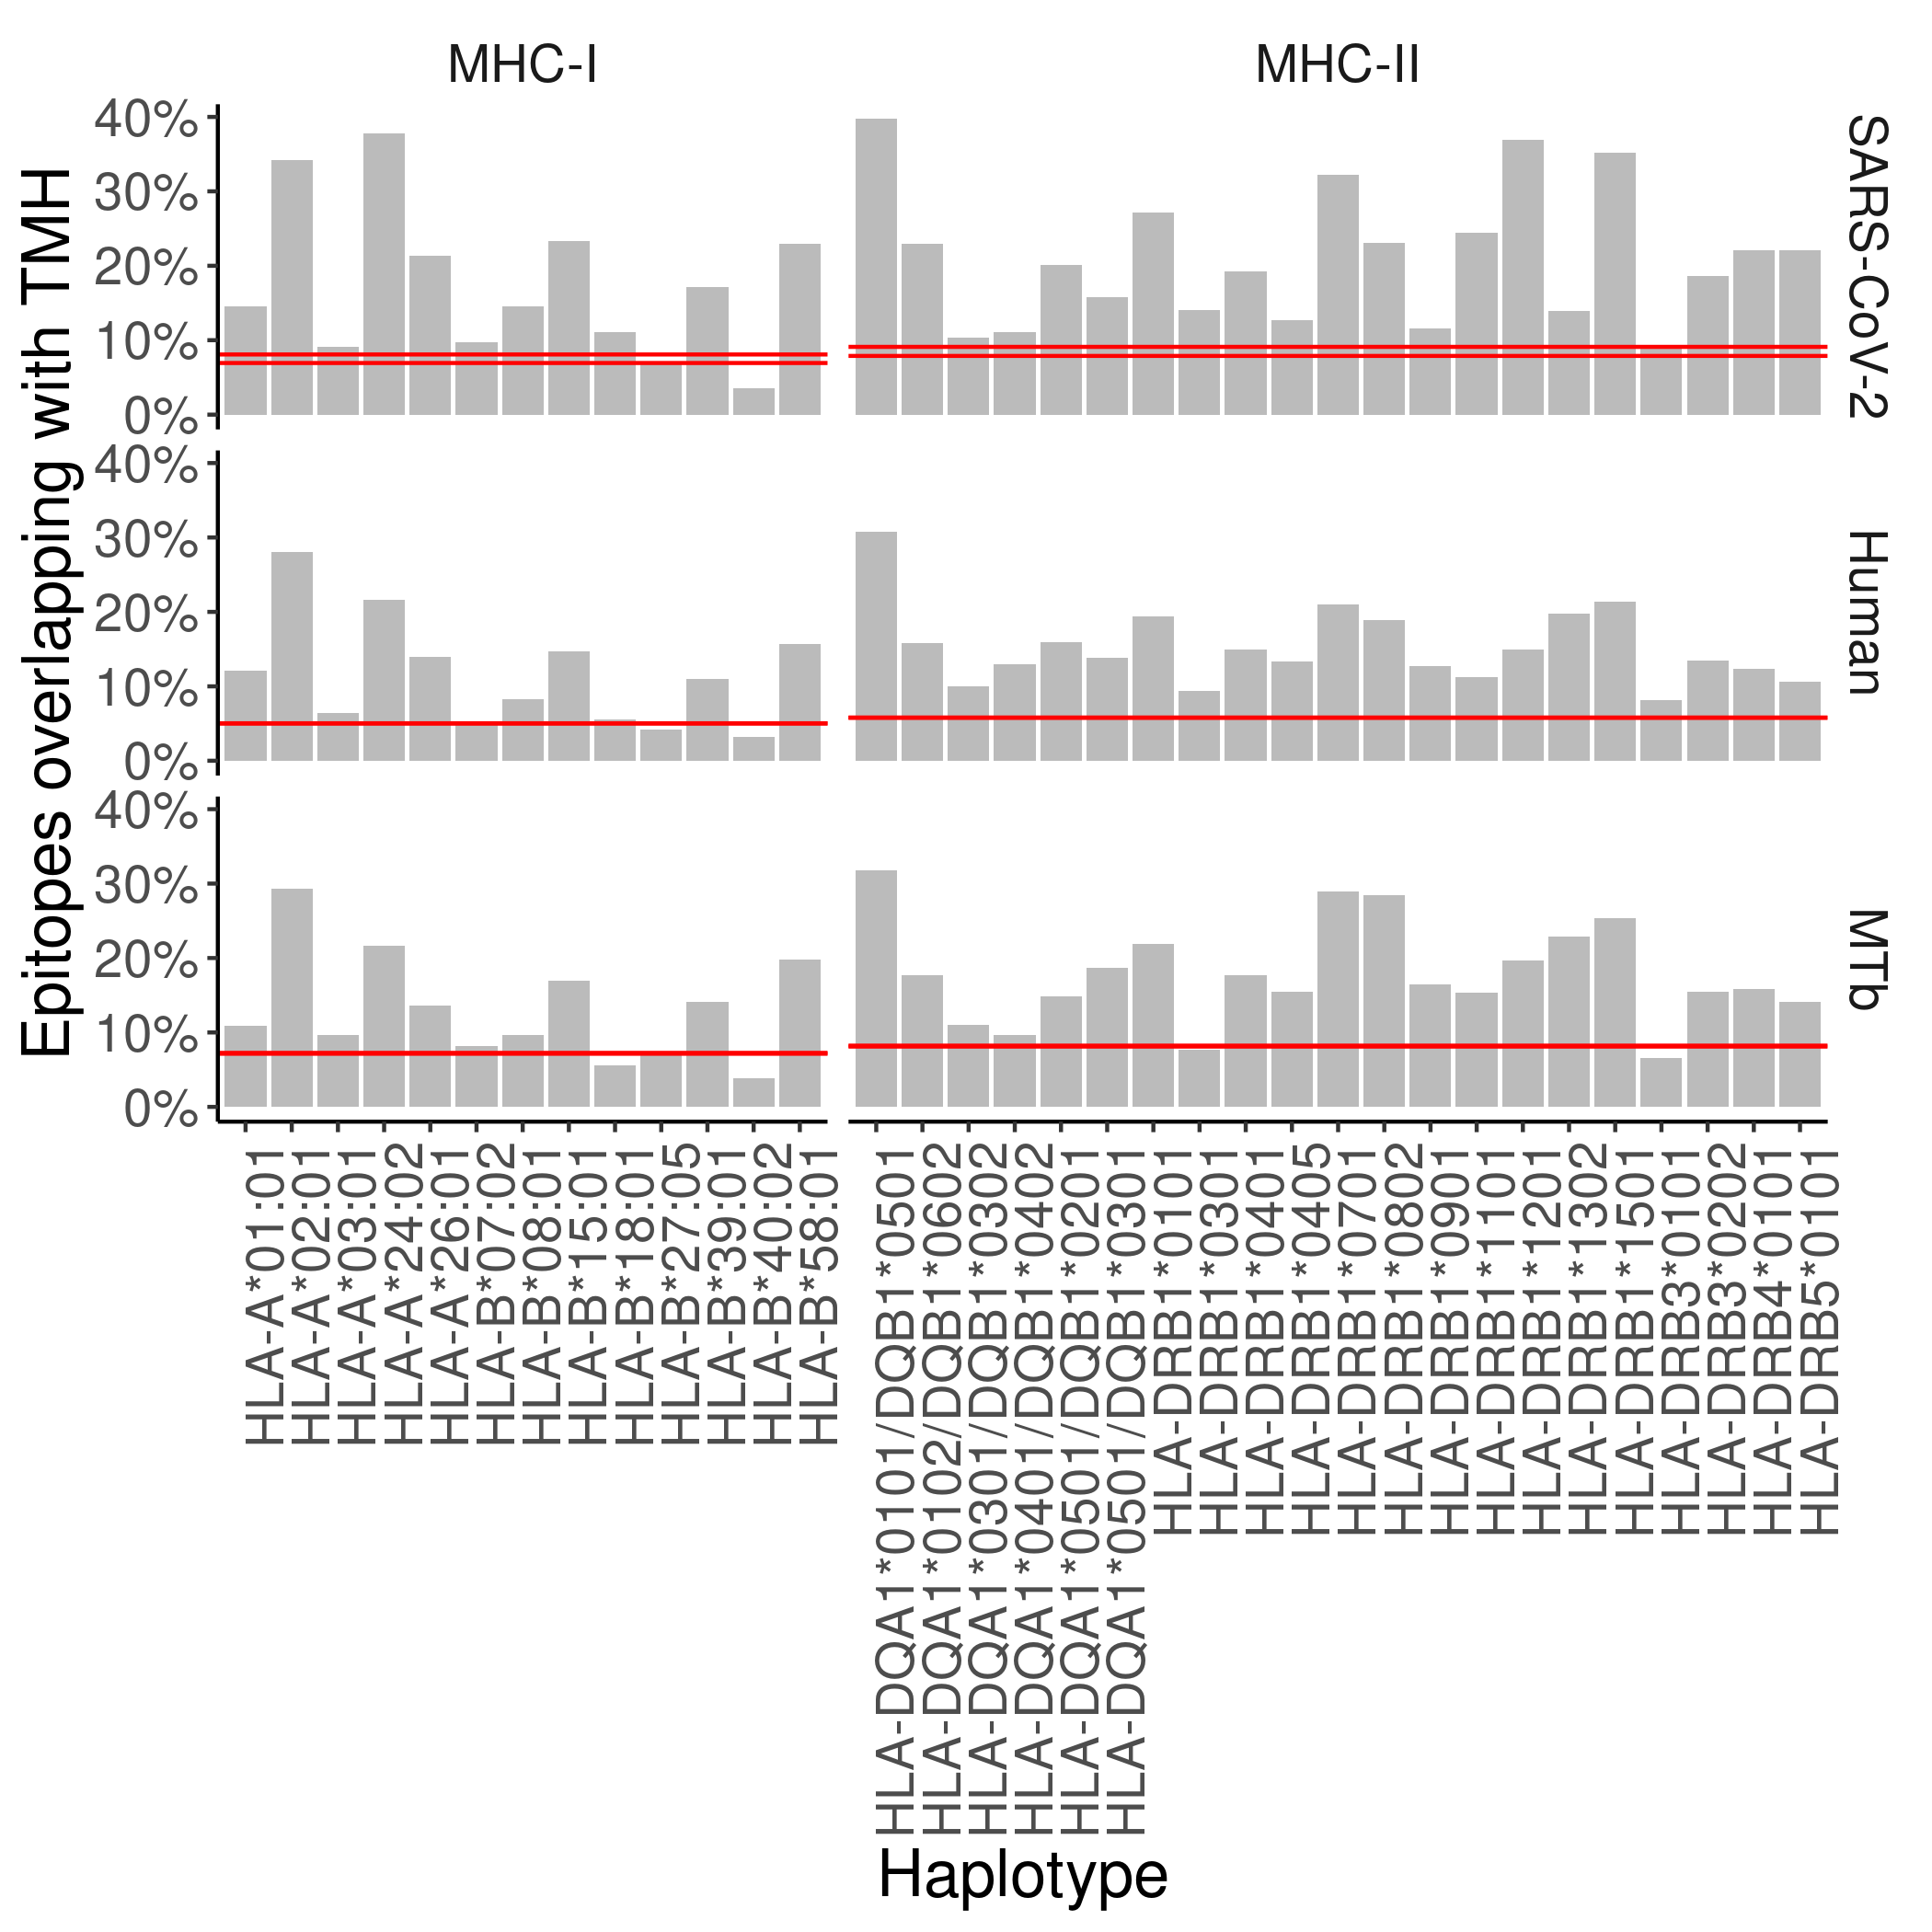
\includegraphics[width=\textwidth]{bbbq_1_smart_2aa_results/fig_f_tmh_2_panel.png}
  \caption{
    The percentage of epitopes for MHC-I and -II haplotypes that are predicted to 
    overlap with TMHs (for at least two amino acids) 
    for the proteomes of SARS-CoV-2 (top row), human (middle 
    row) and \emph{M. tuberculosis} (bottom row).
    The pair of dashed lines in each plot indicate the lower and upper bound of the 99\% confidence interval.
    See supplementary Tables \ref{tab:tmh_binders_mhc2_2aas} and \ref{tab:tmh_binders_mhc1_2aas}
    for the exact TMH and  epitope counts.
  }
  \label{fig:bbbq_1_smart_results_2aas}
\end{figure}

% Label: tab:tmh_binders_mhc2_2aas
\input{bbbq_1_smart_2aa_results/table_tmh_binders_mhc2_2.latex}

% Label: tab:tmh_binders_mhc1_2aas
\input{bbbq_1_smart_2aa_results/table_tmh_binders_mhc1_2.latex}

% Process all floats before going to a next page
\clearpage